\documentclass[12pt]{article}

\usepackage[margin=1in]{geometry}  % set the margins to 1in on all sides
\usepackage{deluxetable}             
\usepackage{graphicx}              % to include figures
\usepackage{amsmath}               % great math stuff
\usepackage{amsfonts}              % for blackboard bold, etc
\usepackage{amsthm}                % better theorem environments
\usepackage{url}

% various theorems, numbered by section

\newtheorem{thm}{Theorem}[section]
\newtheorem{lem}[thm]{Lemma}
\newtheorem{prop}[thm]{Proposition}
\newtheorem{cor}[thm]{Corollary}
\newtheorem{conj}[thm]{Conjecture}
\newtheorem{dfn}[thm]{Definition}

\DeclareMathOperator{\id}{id}

\newcommand{\bd}[1]{\mathbf{#1}}  % for bolding symbols
\newcommand{\RR}{\mathbb{R}}      % for Real numbers
\newcommand{\ZZ}{\mathbb{Z}}      % for Integers
\newcommand{\col}[1]{\left[\begin{matrix} #1 \end{matrix} \right]}
\newcommand{\comb}[2]{\binom{#1^2 + #2^2}{#1+#2}}
	

\begin{document}


\nocite{*}

\title{A Generalized Sphere Theorem for Positively Curved Combinatorial 3-Manifolds}

\author{Aaron Trout \\ Department of Mathematics \\
Chatham University \\ Woodland Rd, Pittsburgh PA 15232 USA \and
Vadas Gintautas\\ Department of Physics \\
Chatham University \\ Woodland Rd, Pittsburgh PA 15232 USA}


\maketitle

\begin{abstract}
The generalized sphere theorem of Grove and Shiohama is an important result in the differential geometry of positively curved manifolds. It shows that if $M$ is a Riemannian manifold whose sectional curvature is everywhere greater than a positive constant and $M$ has diameter greater than half the maximum allowed by the Bonnet-Myers theorem, then $M$ must be homeomorphic to a sphere. In this paper, we present a novel discrete version of this theorem which applies to positively curved {\em combinatorial} 3-manifolds. That is, those with at most five tetrahedra incident at each edge, or equivalently, those with an angle deficit at each edge in the standard piecewise-linear metric. Such spaces have been studied previously and found to satisfy a beautiful discrete version of the Bonnet-Myers theorem. Here, we use a complete census of the positively curved 3-manifolds completed by Lutz and Sullivan to prove a corresponding {\em discrete} generalized sphere theorem.
\end{abstract}


\section{Introduction}

Differential geometry is of central importance not only to geometers but also topologists, physicists and, increasingly, many of those interested in applied topics such as finite element analysis and computer graphics. One significant offshoot in this area is {\em discrete differential geometry} (DDG) which seeks discrete analogues to the classical theorems and concepts from differential geometry. Since many computational treatments of differential geometry involve discretizing shapes, this subject has particular relevance for those with applied interests, see \cite{grinspun2006discrete} for examples. Other recent DDG work with a more pure-mathematics flavor can be found in \cite{BMM,Crowley,EMM,forman2,GGL1,GGL2,GGL3,stone}. 

A particularly important goal in classical differential geometry is to elucidate the relationship between the curvature of a Riemannian (or semi-Riemannian) space and its topology. The classical
results in this area are numerous, elegant, and have inspired an
enormous amount of subsequent research. In this paper, we will present a discrete analogue of the ``generalized'' sphere theorem of Grove and Shiohama \cite{groveshiohama}.

\begin{thm}[Grove-Shiohama] Let $M$ be a complete, connected, $n$-dimensional Riemannian manifold with section curvature $K \geq \delta > 0$ and diameter greater than $\frac{\pi}{2\sqrt{\delta}}$. Then, $M$ is homeomorphic to a sphere.
\label{thm:grove_shiohama}
\end{thm}

\noindent Note that this bound is sharp, since the real projective space $\mathbb{RP}^n$ admits a metric with uniform sectional curvature $K=1$ and diameter $\pi/2$. We should also note also that the diameter bound in Theorem \ref{thm:grove_shiohama} is exactly half the maximum diameter allowed by the Bonnet-Myers theorem:

\begin{thm}[Bonnet-Myers] Let $M$ be a complete, connected, $n$-dimensional Riemannian manifold with sectional curvature $K \geq \delta > 0$. Then the diameter of $M$ is at most $\frac{\pi}{\sqrt{\delta}}$.
\label{thm:bonnet_myers}
\end{thm}

\noindent The main result of this paper is a discrete version of Theorem \ref{thm:grove_shiohama} which is proved by brute-force checking of a combinatorial 3-manifold census created by Lutz and Sullivan \cite{LS}. Before we can state precisely this result, we need a few preliminaries.

\section{Preliminaries}
\label{sect:basics}

The discrete version of Theorem \ref{thm:grove_shiohama} given in this paper will apply to positively curved combinatorial 3-manifolds. A \textbf{combinatorial 3-manifold} $M$ is an abstract simplicial complex in which the link of each vertex is a 2-sphere. We call such a space \textbf{positively curved} if at most five tetrahedra are incident along each edge. Why this terminology? If we endow $M$ with the standard piecewise-linear (PL) metric in which all edges have unit-length, this condition is equivalent to requiring an angle deficit along each edge. In classical differential geometry an angle deficit is intimately related to positive curvature.

A very natural discrete definition of distance in an abstract simplicial complex uses \textbf{edge-paths}. That is, paths entirely contained in the 1-skeleton of $M$. Let $\mathcal{P}_1$ denote the set of all edge-paths on $M$.

\begin{dfn}The \textbf{edge-distance} between two vertices $v$ and $w$ in an abstract simplicial complex $M$ is the minimum length (as a PL-path in the standard PL-metric) of an edge-path from $v$ to $w$. We denote this quantity $d_1(v,w)$. The \textbf{edge-diameter} of $M$, written as $diam_1(M)$, is the maximum of $d_1(v,w)$ over all pairs of vertices $v$ and $w$ in $M$. 
\end{dfn}

\noindent Note that the length of an edge-path is simply the number of edges it traverses.

A discrete version of the Bonnet-Myers theorem was previously proved in \cite{Trout10}. It applies to positively curved combinatorial 3-manifolds and gives a diameter bound in terms of the edge-diameter.

\begin{thm}[Trout] For any connected positively curved combinatorial 3-manifold $M$ we have $diam_1(M)\leq 5$. Moreover, this bound is sharp.
\label{thm:discrete_BM}
\end{thm}

\noindent Interestingly, while the statement of Theorem \ref{thm:discrete_BM} uses edge-diameter, its proof relies on expanding the set of paths under consideration to include those which contain not only edges, but also other types of PL-paths between vertices. In this work, this enlarged set of paths will be crucial to obtaining a discrete result fully analogous to the classical generalized sphere theorem.

\section{Hops and Jumps}
The first new type of path is called a {\em hop}.

\begin{dfn}[Hops] Suppose $\tau$ is a 2-simplex in $M$ and $v_1$ and $v_2$ are vertices in $M$ such that $v_1*\tau$ and $v_2*\tau$ are 3-simplices in $M$. The PL-path from $v_1$ through the barycenter of $\tau$ and ending on $v_2$ will be called a \textbf{hop} from $v_1$ to $v_2$. See Figure \ref{fig:hop} for an illustration.
\end{dfn}

\begin{figure}
	\centering
		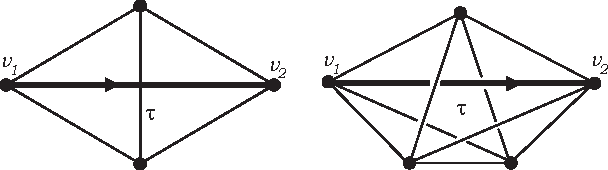
\includegraphics[width=0.28\linewidth]{figures/hops.pdf}
    \caption{A {\em hop} from vertex $v_1$ to vertex $v_2$}
    	\label{fig:hop}
\end{figure}

\noindent The other new type of path we call a {\em jump.}

\begin{dfn}[Jumps] Suppose there are edges $e_1$ and $e_2$ and vertices $v_1$ and $v_2$ in $M$ so that $e_1*e_2$ is a 3-simplex in $M$ and $v_1*e_1$ and $v_2*e_2$ are 2-simplices in $M$. We call the PL-path from $v_1$ through the barycenters of $e_1$ and $e_2$ and ending on $v_2$ a \textbf{jump} from $v_1$ to $v_2$. For an illustration, see Figure \ref{fig:jump}.
\end{dfn}

\begin{figure}
	\centering
		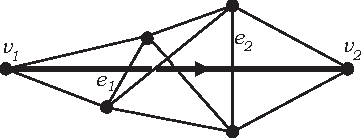
\includegraphics[width=0.36\linewidth]{figures/jump.pdf}
    \caption{A {\em jump} from vertex $v_1$ to vertex $v_2$}
    \label{fig:jump}
\end{figure}

Just as for edges in an edge-path, the length of each hop and jump will be its length as a PL-path in the standard PL metric. Some Euclidean geometry tells us these lengths are \begin{equation} \label{eqn:hop_length} H = \frac{2}{3}\sqrt{2} \end{equation} and \begin{equation} \label{eqn:jump_length} J = \frac{1}{2}\sqrt{2} + \sqrt{3} \end{equation} respectively. We let $d(v,w)$ denote the \textbf{distance between vertices $v$ and $w$} obtained by minimizing over all paths containing edges as well as hops and jumps. Similarly, we let $diam(M)$ denote the \textbf{diameter of $M$} defined in terms of the distance function $d$. Finally, let $\mathcal{P}$ denote the set of all the paths containing edges, hops or jumps.

Why are these paths relevant to this paper? In the classical setting, the generalized sphere theorem requires a manifold to have diameter more than half the maximum allowed by the Bonnet-Myers theorem, and this diameter bound cannot be improved. If we naively imitate the classical results in the discrete setting, from Theorem \ref{thm:discrete_BM} we would want to assume the bound $diam_1(M)>\frac{5}{2}$. Right away we see a discrepancy between the discrete and classical results since this bound cannot possibly be sharp. Worse, the smallest weakening that could be sharp is $diam_1(M) \geq 3$ and this bound does not work. As we will see, there are positively curved combinatorial 3-manifolds $M$ with $diam_1(M)=3$ but which are {\em not} homeomorphic to the 3-sphere. However, if we instead use the finer-grained measure of diameter, $diam(M)$, the problem disappears and the discrete results mirror the classical ones exactly. That is, we can prove a discrete version of the generalized sphere theorem with a diameter bound exactly half the maximum allowed by the corresponding discrete Bonnet-Myers theorem.

What is the discrete Bonnet-Myers theorem corresponding to Theorem \ref{thm:discrete_BM} but which uses $diam(M)$? From the proof of Theorem \ref{thm:discrete_BM} in \cite{Trout10}, we have the following bound on the possible distances which occur in a positively curved 3-manifold.

\begin{lem}[Trout] If $v$ and $w$ are vertices in a connected positively curved combinatorial 3-manifold $M$ then $d(v,w) \in \{0, 1, H, 2, J, 3, 2H, 4, 2J \}$.
\end{lem}

\noindent Note that we have listed the possible distances in increasing numerical order. This result implies the desired discrete Bonnet-Myers type theorem.

\begin{thm}[Trout] For any connected positively curved combinatorial 3-manifold $M$ we have $diam(M) \leq 2J$.
\label{thm:discrete_BM_expanded_paths}
\end{thm}

\noindent Note, it is shown in \cite{Trout10} that this diameter bound is sharp.

\section{Main Results}

We are now able to state our main result.

\begin{thm} Let $M$ be a connected, positively curved, combinatorial 3-manifold. If $M$ has $diam(M)>J$ then it is homeomorphic to a 3-sphere. Moreover, this bound is sharp and equal to half the maximum diameter which occurs for any such $M$.
\label{thm:discrete_GS}
\end{thm}

\noindent The proof of this theorem relies on the work of Lutz, Sullivan and Sulanke in \cite{Lutz07, LutzSul_unpub, sulanke2009isomorphism} who created a complete census of positively curved combinatorial 3-manifolds along with a list of their topological types. See \cite{Lutz_online_manifolds} and \cite{Lutz_online_topological_types}. This census contains 4787 manifolds, with the following topologies represented: the 3-sphere $S^3$, the real projective space $\mathbb{RP}^3$, the lens spaces $L(3,1)$ and $L(4,1)$, and the cube space $S^3/Q$. Note that all of these manifolds are homeomorphic to either a 3-sphere or to the quotient space of a 3-sphere under the action of a finite group. 

Python programs (available on request) were written to examine each manifold in the census and compute its diameter and edge-diameter. See Figure \ref{fig:type_statistics} for a plot of the number of manifolds by topological type and diameter. As claimed, every manifold with diameter greater than $J$ is a 3-sphere. The corresponding data using the coarser-grained edge-diameter can be found in Figure \ref{fig:type_statistics_edges}. Note the existence of $3$-manifolds with edge-diameter greater than half the maximum allowed edge-diameter and which are {\em not} homeomorphic to the 3-sphere.

When only edge-paths are considered, as expected we obtain the following result from the census:

\begin{thm} If $M$ is a connected, positively curved, combinatorial 3-manifold satisfying the bound $diam_1(M) > 3$ then $M$ is homeomorphic to the 3-sphere. Moreover, this bound is sharp.
\end{thm}

\begin{figure}
    \begin{center}
    {
	    \setlength\fboxsep{15pt}
		\setlength\fboxrule{0pt}
		\fbox{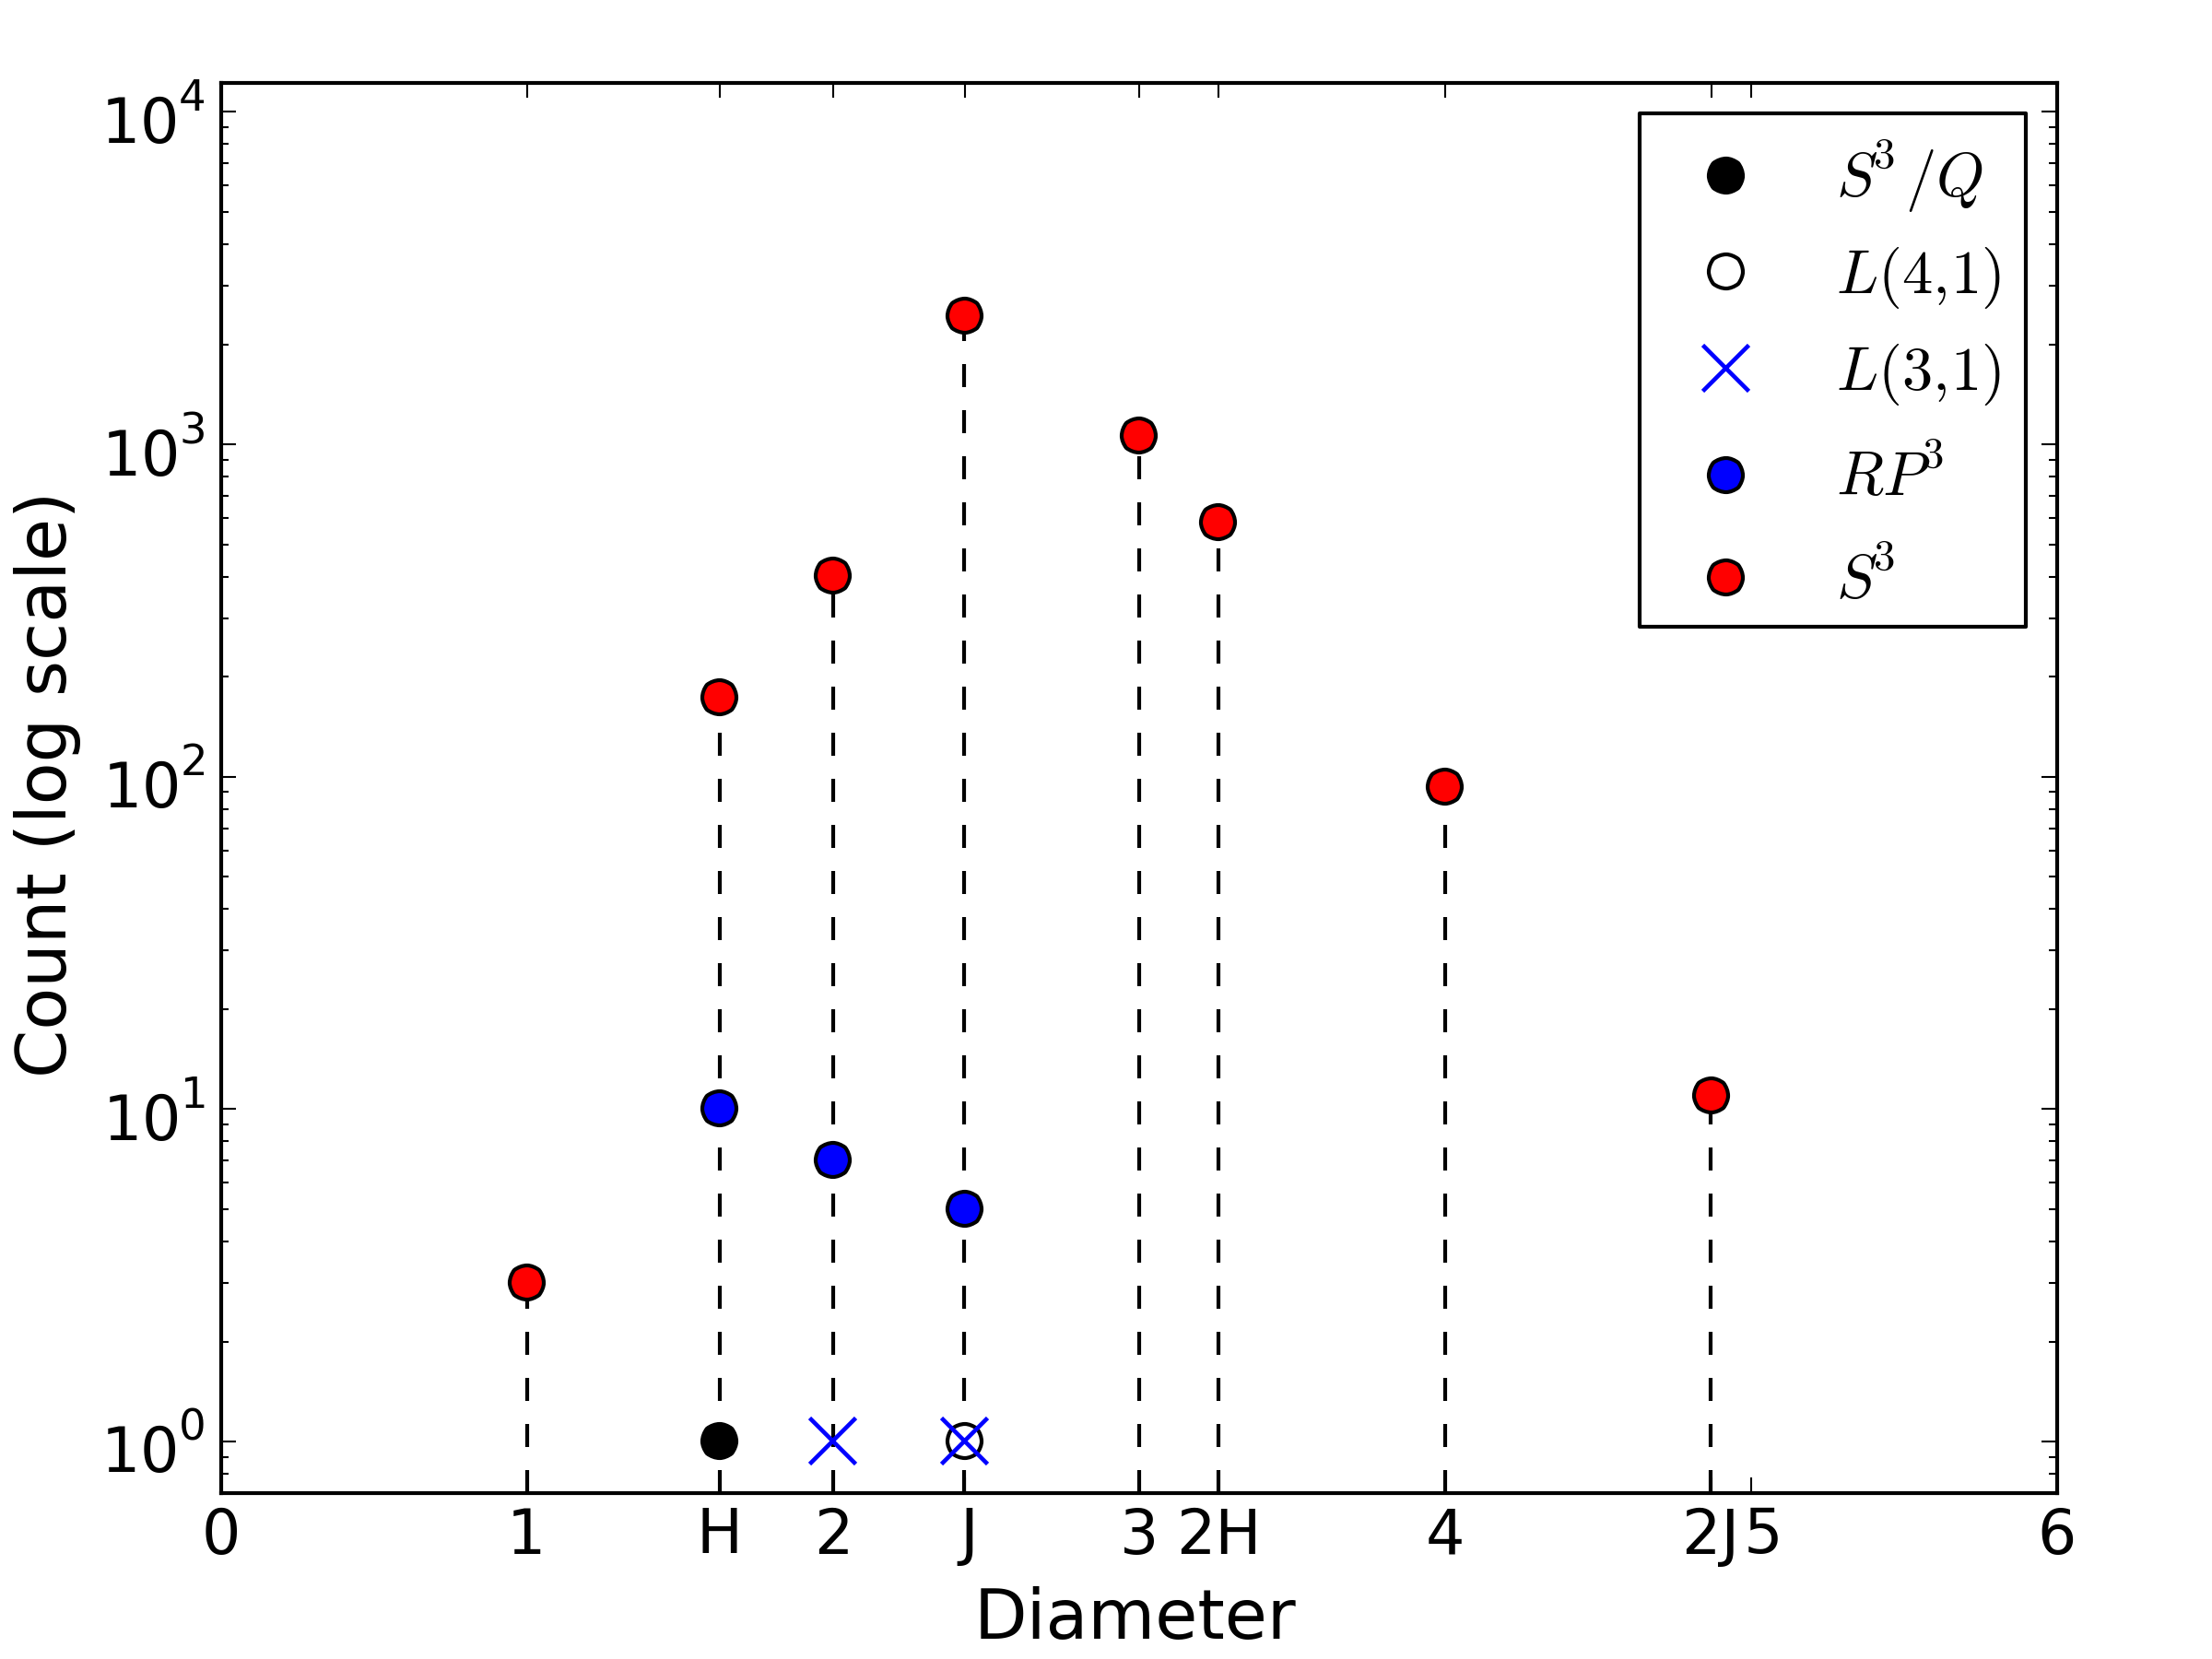
\includegraphics[width=0.9\linewidth]{figures/split_statistics.png}}
    }
    	\renewcommand{\arraystretch}{1.2}
    \begin{tabular} {| r | r | r | r | r | r | r |}
		\hline
		Diameter & $S^{3}/Q$ & $L(4,1)$ & $L(3,1)$ & $RP^{3}$ & $S^{3}$ & Total \\
		\hline
		\hline
		$1$&  &  &  &   &3    & 3    \\
		$H$&1 &  &  &10 &173  & 184  \\
		$2$&  &  &1 &7  &401  & 409  \\
		$J$&  &1 &1 &5  &2438 & 2445 \\
		$3$&  &  &  &   &1060 & 1060 \\
		$2H$&  &  &  &   &582  & 582  \\
		$4$&  &  &  &   &93   & 93   \\
		$2J$&  &  &  &   &11   & 11   \\
		\hline
		Total&1 &1 &2 &22   &4761   &4787  \\
		\hline
	\end{tabular}
    \end{center}
    \caption{Number of connected positively curved combinatorial 3-manifolds by topology and diameter, displayed graphically (above) and in table form (below). Note that all manifolds with diameter greater than half the maximum are 3-spheres. Results were computed using a 3-manifold census created by Lutz and Sullivan \cite{LutzSul_unpub}.}
    \label{fig:type_statistics}
\end{figure}

\begin{figure}
    \begin{center}
    {
	    \setlength\fboxsep{15pt}
		\setlength\fboxrule{0pt}
		\fbox{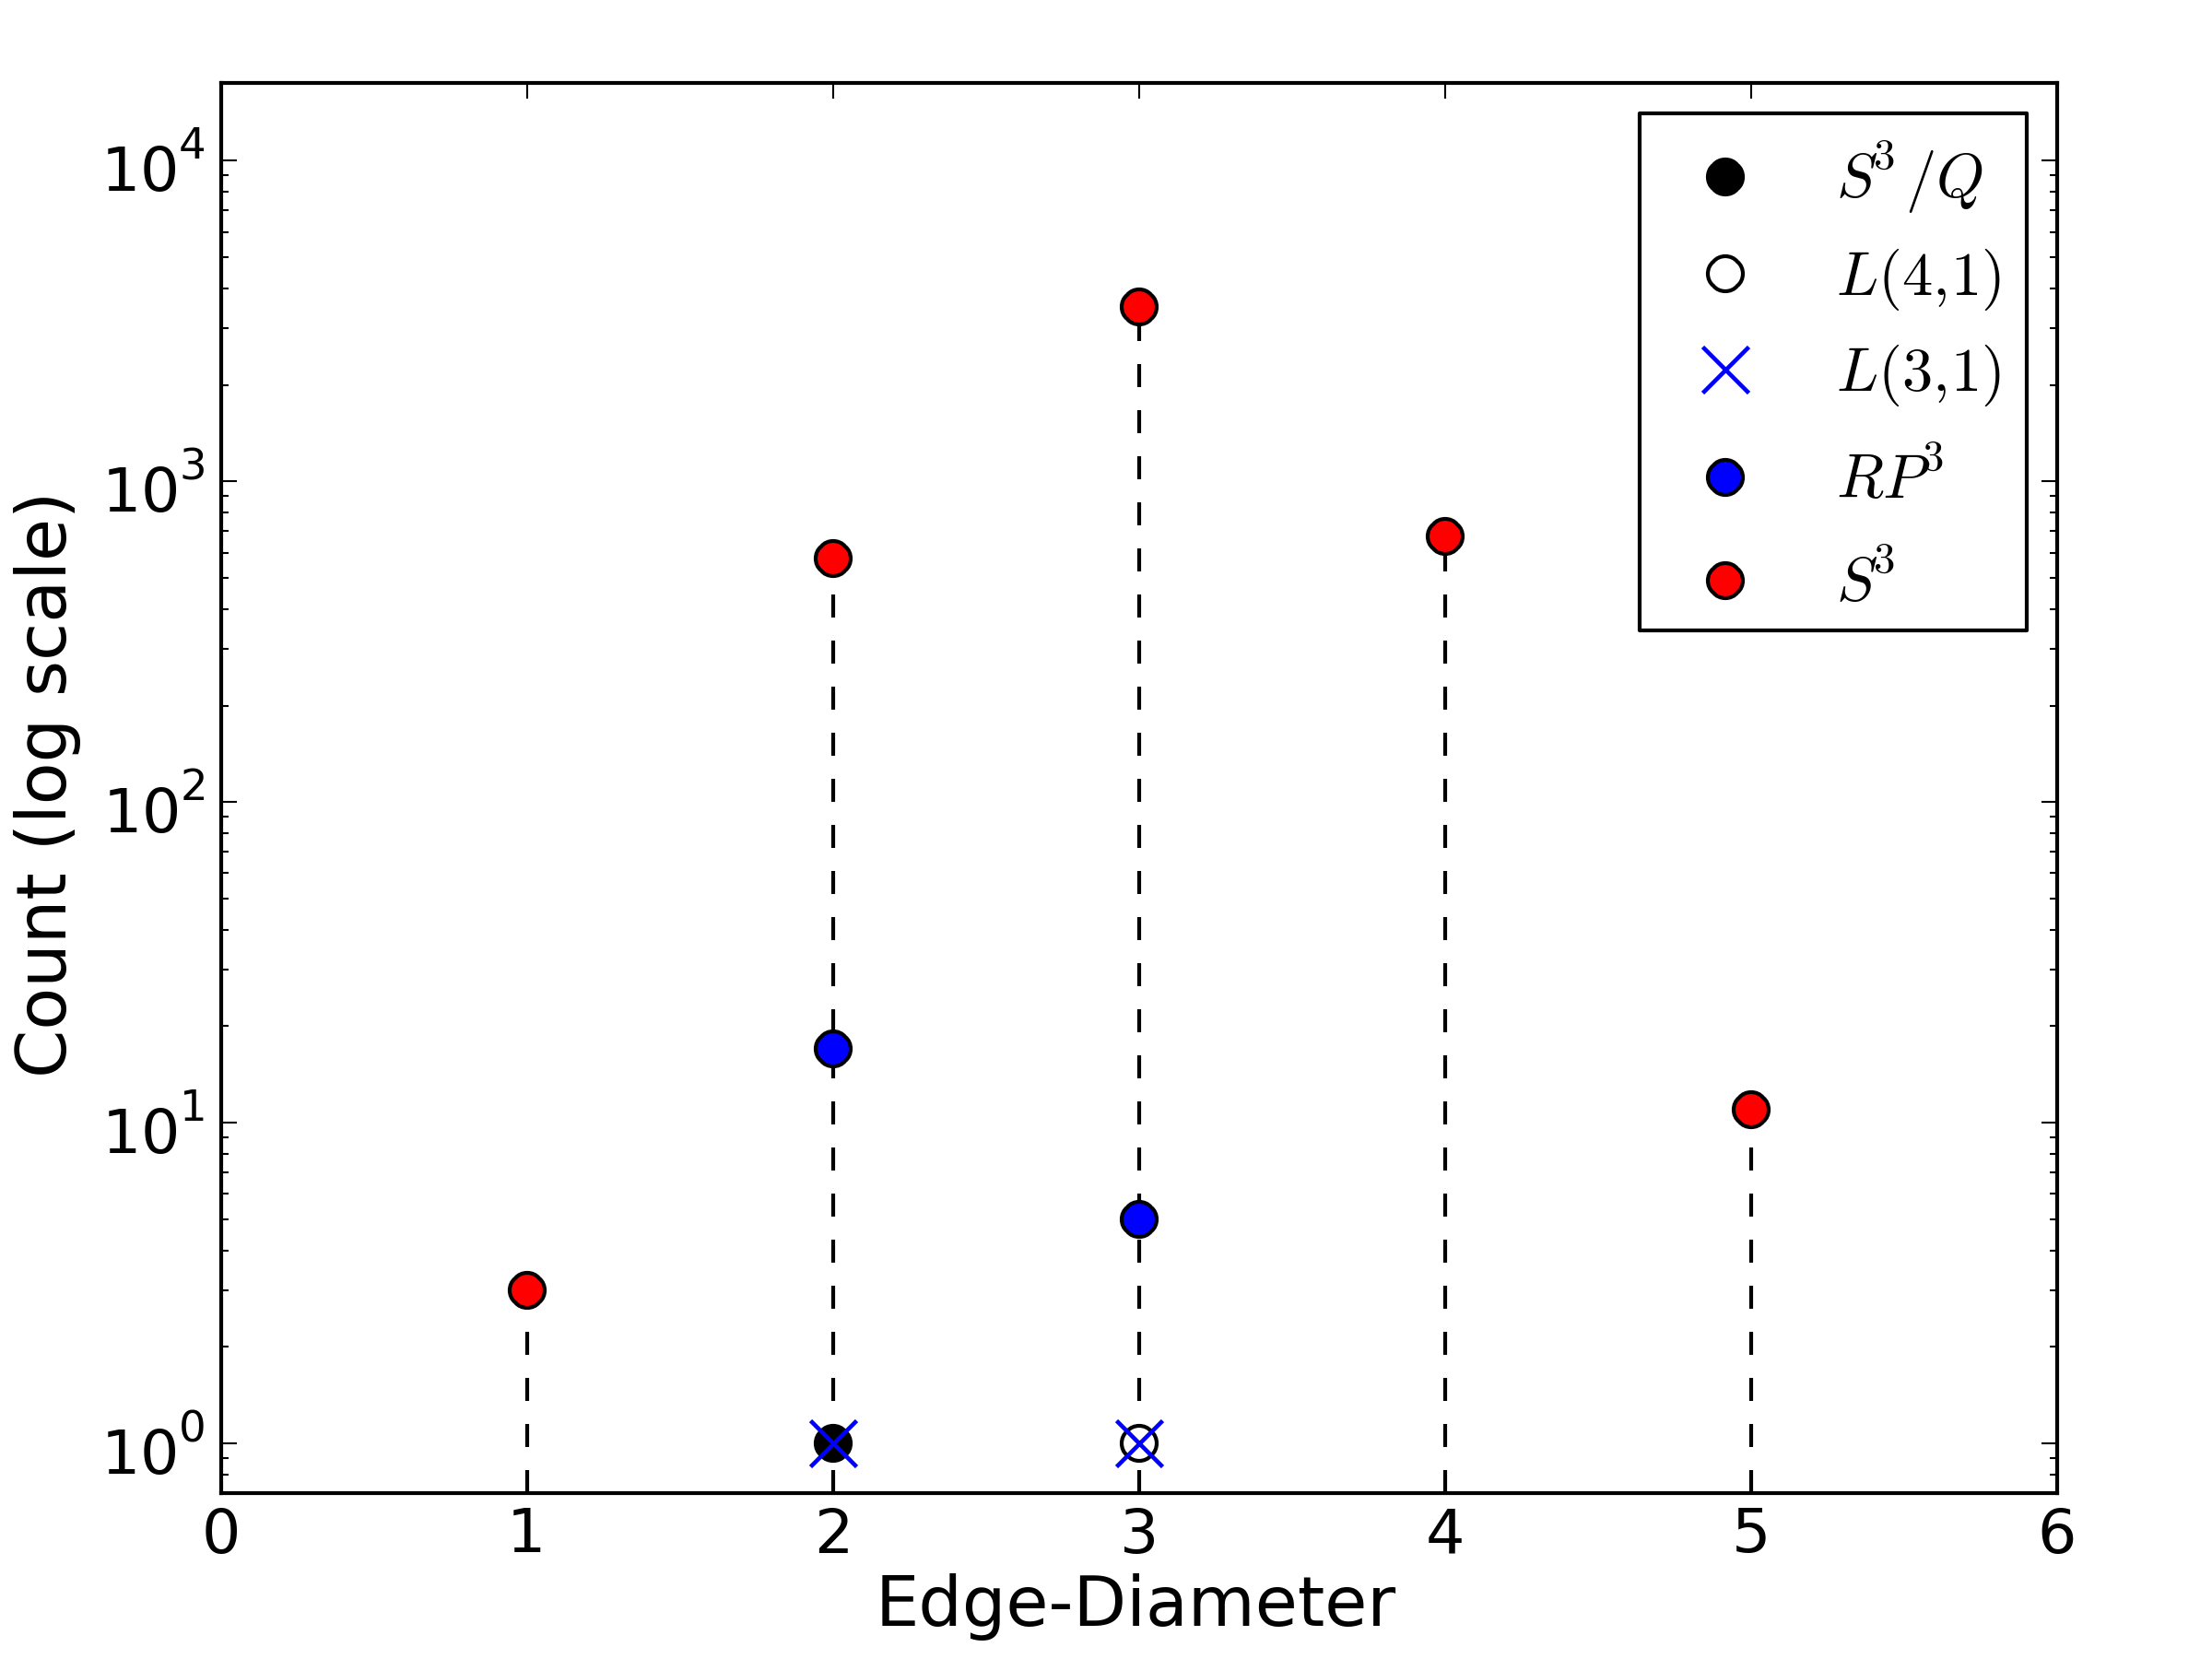
\includegraphics[width=0.9\linewidth]{figures/split_edge_diameters.png}}
    }
    \renewcommand{\arraystretch}{1.2}
	\begin{tabular} {| r | r | r | r | r | r | r |}	
		\hline
		Edge-Diameter & $S^{3}/Q$ & $L(4,1)$ & $L(3,1)$ & $RP^{3}$ & $S^{3}$ & Total \\
		\hline
		\hline
		$1$ &  &  &  &   &3    & 3    \\
		$2$ & 1&  &1 &17 &574  & 593  \\
		$3$ &  &1 &1 &5  &3498 & 3505 \\
		$4$ &  &  &  &   &675  & 675   \\
		$5$ &  &  &  &   &11   & 11   \\
		\hline
		Total&1 &1 &2 &22   &4761   &4787  \\
		\hline
	\end{tabular}
    \end{center}
    \caption{Number of connected positively curved combinatorial 3-manifolds by topology and edge-diameter, displayed graphically (above) and in table form (below). Note that when diameters are measured in edges, there are manifolds with diameter greater than half the maximum which are {\em not} 3-spheres. Results were computed using a 3-manifold census created by Lutz and Sullivan \cite{LutzSul_unpub}.}
	\label{fig:type_statistics_edges}
\end{figure}

\section{Discussion}
We should mention another notable advantage of expanding the space of paths to include hops and edges. In classical differential geometry, a geodesic segment is completely determined by its the starting point, initial direction, and length. There is no ``branching'' of geodesics on a Riemannian manifold. Indeed, this property is of fundamental importance to constructing many arguments in this area. However in the discrete setting, if we use only edge-paths then this valuable characteristic does not hold. It is possible to have two minimal edge-paths with the same length and which begin by traversing the same edge, yet reach distinct destination vertices.

To see this, consider a combinatorial 3-manifold $M$ containing a minimal jump from vertex $v$ to vertex $w$ passing through edges $e_1$ and $e_2$ (as seen in Figure \ref{fig:jump}.) Using the structure of a jump, we will construct two edge-paths starting at $v$. We choose the first edge from $v$ to some vertex in $e_1$ and then we can continue the path to either of the vertices in $e_2$. The resulting paths, $Q_1$ and $Q_2$, must be minimal among edge-paths. If they were not, then their endpoints would be connected by an edge and a two-edge path from $v$ to $w$ would exist, contradicting the minimality of the jump. Thus $Q_1$ and $Q_2$ provide examples of minimal edge-paths which ``branch''. The non-branching property of minimal paths is restored, at least for positively curved manifolds, if we include hops and jumps. In particular we have:

\begin{thm}(Unique Extension) If two minimal paths $P_1$ and $P_2$ in $\mathcal{P}$ pass through the same first two simplices of a positively curved 3-manifold $M$ and $P_1$ and $P_2$ have the same length, then $P_1 = P_2$. This result is false if $\mathcal{P}$ is replaced by $\mathcal{P}_1$.
\end{thm}

\noindent See \cite{Trout10} for details.

It is not entirely surprising that discrete differential geometry on a PL-manifold $M$ comes to resemble classical differential geometry more and more as the set of admissible PL-paths on $M$ is expanded. Forcing ourselves to use only edges amounts to coarse-graining the underlying PL-geometry, and expanding the set of paths clearly reduces this coarse-graining. We could even include {\em all} the PL-paths in $M$ and still have a ``discrete'' geometry in some sense, because our PL-metric is determined solely by the structure of $M$ as a simplicial complex. However, since PL-paths admit infinitesimal deformations we would lose much of the ``discrete'' flavor to the theory. The successful use of hops and jumps in this paper and in \cite{Trout10} indicate that one can improve the behavior of discrete geometries by judicious inclusion of PL-paths in addition to edges. Investigating the possibilities for such inclusions and their benefits represents an exciting topic of further research.
\bibliographystyle{plain}
\bibliography{manifolds}


\begin{deluxetable}{|llr||llr||llr||llr||llr|}
\tablewidth{0pc}
\tablecolumns{15}
\tablecaption{Awesome results\label{tab:full}}
\tablehead{
$N$ & $t$ & $d$ &$N$ & $t$ & $d$ &$N$ & $t$ & $d$ &$N$ & $t$ & $d$ &$N$ & $t$ & $d$   }
\startdata
1 & $S^3$ & $1 $
 & 959 & $S^3$ & $J$
 & 1917 & $S^3$ & $J$
 & 2875 & $S^3$ & $J$
 & 3833 & $S^3$ & $J$
\\
2 & $S^3$ & $H $
 & 960 & $S^3$ & $J$
 & 1918 & $S^3$ & $2 $
 & 2876 & $S^3$ & $J$
 & 3834 & $S^3$ & $J$
\\
3 & $S^3$ & $H $
 & 961 & $S^3$ & $J$
 & 1919 & $S^3$ & $2 $
 & 2877 & $S^3$ & $2 $
 & 3835 & $S^3$ & $J$
\\
4 & $S^3$ & $H $
 & 962 & $S^3$ & $J$
 & 1920 & $S^3$ & $2 $
 & 2878 & $S^3$ & $J$
 & 3836 & $S^3$ & $J$
\\
5 & $S^3$ & $H $
 & 963 & $S^3$ & $2H $
 & 1921 & $S^3$ & $2 $
 & 2879 & $S^3$ & $J$
 & 3837 & $S^3$ & $J$
\\
6 & $S^3$ & $H $
 & 964 & $S^3$ & $2H $
 & 1922 & $S^3$ & $2 $
 & 2880 & $S^3$ & $J$
 & 3838 & $S^3$ & $2 $
\\
7 & $S^3$ & $J$
 & 965 & $S^3$ & $2H $
 & 1923 & $S^3$ & $2 $
 & 2881 & $S^3$ & $J$
 & 3839 & $S^3$ & $J$
\\
8 & $S^3$ & $2 $
 & 966 & $S^3$ & $J$
 & 1924 & $S^3$ & $2 $
 & 2882 & $S^3$ & $J$
 & 3840 & $S^3$ & $J$
\\
9 & $S^3$ & $2 $
 & 967 & $S^3$ & $3 $
 & 1925 & $S^3$ & $J$
 & 2883 & $S^3$ & $J$
 & 3841 & $S^3$ & $J$
\\
10 & $S^3$ & $2 $
 & 968 & $S^3$ & $2H $
 & 1926 & $S^3$ & $J$
 & 2884 & $S^3$ & $J$
 & 3842 & $S^3$ & $J$
\\
11 & $S^3$ & $J$
 & 969 & $S^3$ & $2H $
 & 1927 & $S^3$ & $2 $
 & 2885 & $S^3$ & $J$
 & 3843 & $S^3$ & $J$
\\
12 & $S^3$ & $H $
 & 970 & $S^3$ & $2H $
 & 1928 & $S^3$ & $2 $
 & 2886 & $S^3$ & $J$
 & 3844 & $S^3$ & $J$
\\
13 & $S^3$ & $2 $
 & 971 & $S^3$ & $3 $
 & 1929 & $S^3$ & $J$
 & 2887 & $S^3$ & $J$
 & 3845 & $S^3$ & $J$
\\
14 & $S^3$ & $2 $
 & 972 & $S^3$ & $J$
 & 1930 & $S^3$ & $J$
 & 2888 & $S^3$ & $J$
 & 3846 & $S^3$ & $J$
\\
15 & $S^3$ & $2 $
 & 973 & $S^3$ & $2H $
 & 1931 & $S^3$ & $J$
 & 2889 & $S^3$ & $3 $
 & 3847 & $S^3$ & $3 $
\\
16 & $S^3$ & $J$
 & 974 & $S^3$ & $J$
 & 1932 & $S^3$ & $J$
 & 2890 & $S^3$ & $2H $
 & 3848 & $S^3$ & $3 $
\\
17 & $S^3$ & $2 $
 & 975 & $S^3$ & $2H $
 & 1933 & $S^3$ & $2 $
 & 2891 & $S^3$ & $J$
 & 3849 & $S^3$ & $2 $
\\
18 & $S^3$ & $J$
 & 976 & $S^3$ & $2H $
 & 1934 & $S^3$ & $J$
 & 2892 & $S^3$ & $J$
 & 3850 & $S^3$ & $J$
\\
19 & $S^3$ & $J$
 & 977 & $S^3$ & $3 $
 & 1935 & $S^3$ & $J$
 & 2893 & $S^3$ & $3 $
 & 3851 & $S^3$ & $J$
\\
20 & $S^3$ & $J$
 & 978 & $S^3$ & $2H $
 & 1936 & $S^3$ & $J$
 & 2894 & $S^3$ & $J$
 & 3852 & $S^3$ & $J$
\\
21 & $S^3$ & $2 $
 & 979 & $S^3$ & $3 $
 & 1937 & $S^3$ & $J$
 & 2895 & $S^3$ & $J$
 & 3853 & $S^3$ & $2 $
\\
22 & $S^3$ & $J$
 & 980 & $S^3$ & $2H $
 & 1938 & $S^3$ & $2 $
 & 2896 & $S^3$ & $3 $
 & 3854 & $S^3$ & $J$
\\
23 & $S^3$ & $3 $
 & 981 & $S^3$ & $3 $
 & 1939 & $S^3$ & $J$
 & 2897 & $S^3$ & $3 $
 & 3855 & $S^3$ & $J$
\\
24 & $S^3$ & $J$
 & 982 & $S^3$ & $2H $
 & 1940 & $S^3$ & $H $
 & 2898 & $S^3$ & $2H $
 & 3856 & $S^3$ & $J$
\\
25 & $S^3$ & $J$
 & 983 & $S^3$ & $3 $
 & 1941 & $S^3$ & $2 $
 & 2899 & $S^3$ & $2H $
 & 3857 & $S^3$ & $J$
\\
26 & $S^3$ & $J$
 & 984 & $S^3$ & $3 $
 & 1942 & $S^3$ & $2 $
 & 2900 & $RP^3$ & $H $
 & 3858 & $S^3$ & $J$
\\
27 & $S^3$ & $J$
 & 985 & $S^3$ & $3 $
 & 1943 & $S^3$ & $J$
 & 2901 & $S^3$ & $2 $
 & 3859 & $S^3$ & $J$
\\
28 & $S^3$ & $3 $
 & 986 & $S^3$ & $2H $
 & 1944 & $S^3$ & $J$
 & 2902 & $RP^3$ & $2 $
 & 3860 & $S^3$ & $J$
\\
29 & $S^3$ & $3 $
 & 987 & $S^3$ & $3 $
 & 1945 & $S^3$ & $2 $
 & 2903 & $S^3$ & $2 $
 & 3861 & $S^3$ & $2 $
\\
30 & $S^3$ & $2H $
 & 988 & $S^3$ & $2H $
 & 1946 & $S^3$ & $J$
 & 2904 & $S^3$ & $J$
 & 3862 & $S^3$ & $J$
\\
31 & $S^3$ & $4 $
 & 989 & $S^3$ & $2H $
 & 1947 & $S^3$ & $J$
 & 2905 & $S^3$ & $J$
 & 3863 & $S^3$ & $J$
\\
32 & $S^3$ & $2 $
 & 990 & $S^3$ & $4 $
 & 1948 & $S^3$ & $J$
 & 2906 & $S^3$ & $J$
 & 3864 & $S^3$ & $J$
\\
33 & $S^3$ & $3 $
 & 991 & $S^3$ & $4 $
 & 1949 & $S^3$ & $2 $
 & 2907 & $S^3$ & $2 $
 & 3865 & $S^3$ & $J$
\\
34 & $S^3$ & $J$
 & 992 & $S^3$ & $4 $
 & 1950 & $S^3$ & $2 $
 & 2908 & $S^3$ & $2 $
 & 3866 & $S^3$ & $3 $
\\
35 & $S^3$ & $J$
 & 993 & $S^3$ & $J$
 & 1951 & $S^3$ & $2 $
 & 2909 & $S^3$ & $2 $
 & 3867 & $S^3$ & $3 $
\\
36 & $S^3$ & $3 $
 & 994 & $S^3$ & $3 $
 & 1952 & $RP^3$ & $H $
 & 2910 & $S^3$ & $2 $
 & 3868 & $S^3$ & $J$
\\
37 & $S^3$ & $J$
 & 995 & $S^3$ & $J$
 & 1953 & $S^3$ & $2 $
 & 2911 & $S^3$ & $J$
 & 3869 & $RP^3$ & $H $
\\
38 & $S^3$ & $J$
 & 996 & $S^3$ & $J$
 & 1954 & $S^3$ & $2 $
 & 2912 & $S^3$ & $J$
 & 3870 & $RP^3$ & $H $
\\
39 & $S^3$ & $2H $
 & 997 & $S^3$ & $J$
 & 1955 & $S^3$ & $2 $
 & 2913 & $S^3$ & $2 $
 & 3871 & $S^3$ & $2 $
\\
40 & $S^3$ & $3 $
 & 998 & $S^3$ & $J$
 & 1956 & $S^3$ & $J$
 & 2914 & $S^3$ & $J$
 & 3872 & $S^3$ & $J$
\\
41 & $S^3$ & $2H $
 & 999 & $S^3$ & $3 $
 & 1957 & $S^3$ & $2 $
 & 2915 & $S^3$ & $2 $
 & 3873 & $S^3$ & $J$
\\
42 & $S^3$ & $3 $
 & 1000 & $S^3$ & $3 $
 & 1958 & $S^3$ & $2 $
 & 2916 & $S^3$ & $J$
 & 3874 & $S^3$ & $J$
\\
43 & $S^3$ & $2H $
 & 1001 & $S^3$ & $3 $
 & 1959 & $S^3$ & $2 $
 & 2917 & $S^3$ & $J$
 & 3875 & $S^3$ & $J$
\\
44 & $S^3$ & $4 $
 & 1002 & $S^3$ & $J$
 & 1960 & $S^3$ & $J$
 & 2918 & $S^3$ & $J$
 & 3876 & $S^3$ & $J$
\\
45 & $S^3$ & $2J$
 & 1003 & $S^3$ & $J$
 & 1961 & $S^3$ & $J$
 & 2919 & $S^3$ & $J$
 & 3877 & $S^3$ & $J$
\\
46 & $S^3$ & $1 $
 & 1004 & $S^3$ & $3 $
 & 1962 & $S^3$ & $J$
 & 2920 & $S^3$ & $J$
 & 3878 & $S^3$ & $J$
\\
47 & $S^3$ & $H $
 & 1005 & $S^3$ & $3 $
 & 1963 & $S^3$ & $2 $
 & 2921 & $S^3$ & $J$
 & 3879 & $S^3$ & $J$
\\
48 & $S^3$ & $H $
 & 1006 & $S^3$ & $3 $
 & 1964 & $S^3$ & $2 $
 & 2922 & $S^3$ & $2 $
 & 3880 & $S^3$ & $J$
\\
49 & $S^3$ & $H $
 & 1007 & $S^3$ & $3 $
 & 1965 & $S^3$ & $2 $
 & 2923 & $S^3$ & $J$
 & 3881 & $S^3$ & $J$
\\
50 & $S^3$ & $H $
 & 1008 & $S^3$ & $J$
 & 1966 & $S^3$ & $2 $
 & 2924 & $S^3$ & $J$
 & 3882 & $S^3$ & $J$
\\
51 & $S^3$ & $H $
 & 1009 & $S^3$ & $2H $
 & 1967 & $S^3$ & $2 $
 & 2925 & $S^3$ & $2 $
 & 3883 & $S^3$ & $J$
\\
52 & $S^3$ & $H $
 & 1010 & $S^3$ & $3 $
 & 1968 & $S^3$ & $J$
 & 2926 & $S^3$ & $2 $
 & 3884 & $S^3$ & $J$
\\
53 & $S^3$ & $2 $
 & 1011 & $S^3$ & $3 $
 & 1969 & $S^3$ & $J$
 & 2927 & $S^3$ & $J$
 & 3885 & $S^3$ & $3 $
\\
54 & $S^3$ & $H $
 & 1012 & $S^3$ & $3 $
 & 1970 & $S^3$ & $J$
 & 2928 & $S^3$ & $J$
 & 3886 & $S^3$ & $3 $
\\
55 & $S^3$ & $H $
 & 1013 & $RP^3$ & $J$
 & 1971 & $S^3$ & $J$
 & 2929 & $S^3$ & $J$
 & 3887 & $S^3$ & $J$
\\
56 & $S^3$ & $H $
 & 1014 & $S^3$ & $2H $
 & 1972 & $S^3$ & $2 $
 & 2930 & $S^3$ & $J$
 & 3888 & $S^3$ & $3 $
\\
57 & $S^3$ & $H $
 & 1015 & $S^3$ & $2H $
 & 1973 & $S^3$ & $J$
 & 2931 & $S^3$ & $3 $
 & 3889 & $S^3$ & $3 $
\\
58 & $S^3$ & $H $
 & 1016 & $S^3$ & $2H $
 & 1974 & $S^3$ & $J$
 & 2932 & $S^3$ & $J$
 & 3890 & $S^3$ & $3 $
\\
59 & $S^3$ & $H $
 & 1017 & $S^3$ & $3 $
 & 1975 & $S^3$ & $J$
 & 2933 & $S^3$ & $J$
 & 3891 & $S^3$ & $3 $
\\
60 & $S^3$ & $2 $
 & 1018 & $S^3$ & $3 $
 & 1976 & $S^3$ & $J$
 & 2934 & $S^3$ & $J$
 & 3892 & $S^3$ & $3 $
\\
61 & $S^3$ & $2 $
 & 1019 & $S^3$ & $2H $
 & 1977 & $S^3$ & $J$
 & 2935 & $S^3$ & $J$
 & 3893 & $S^3$ & $J$
\\
62 & $S^3$ & $J$
 & 1020 & $S^3$ & $2H $
 & 1978 & $S^3$ & $2 $
 & 2936 & $S^3$ & $J$
 & 3894 & $S^3$ & $J$
\\
63 & $S^3$ & $H $
 & 1021 & $S^3$ & $2H $
 & 1979 & $S^3$ & $J$
 & 2937 & $S^3$ & $2 $
 & 3895 & $S^3$ & $J$
\\
64 & $S^3$ & $H $
 & 1022 & $S^3$ & $3 $
 & 1980 & $S^3$ & $J$
 & 2938 & $S^3$ & $J$
 & 3896 & $S^3$ & $J$
\\
65 & $S^3$ & $H $
 & 1023 & $S^3$ & $2H $
 & 1981 & $S^3$ & $J$
 & 2939 & $S^3$ & $J$
 & 3897 & $S^3$ & $J$
\\
66 & $S^3$ & $H $
 & 1024 & $S^3$ & $3 $
 & 1982 & $S^3$ & $J$
 & 2940 & $S^3$ & $J$
 & 3898 & $S^3$ & $J$
\\
67 & $S^3$ & $H $
 & 1025 & $S^3$ & $2H $
 & 1983 & $S^3$ & $J$
 & 2941 & $S^3$ & $J$
 & 3899 & $S^3$ & $3 $
\\
68 & $S^3$ & $H $
 & 1026 & $S^3$ & $2H $
 & 1984 & $S^3$ & $J$
 & 2942 & $S^3$ & $J$
 & 3900 & $S^3$ & $J$
\\
69 & $S^3$ & $2 $
 & 1027 & $S^3$ & $2H $
 & 1985 & $S^3$ & $J$
 & 2943 & $S^3$ & $J$
 & 3901 & $S^3$ & $J$
\\
70 & $S^3$ & $J$
 & 1028 & $S^3$ & $2H $
 & 1986 & $S^3$ & $J$
 & 2944 & $S^3$ & $J$
 & 3902 & $S^3$ & $3 $
\\
71 & $S^3$ & $H $
 & 1029 & $S^3$ & $3 $
 & 1987 & $S^3$ & $J$
 & 2945 & $S^3$ & $2 $
 & 3903 & $S^3$ & $3 $
\\
72 & $S^3$ & $H $
 & 1030 & $S^3$ & $2H $
 & 1988 & $S^3$ & $2 $
 & 2946 & $S^3$ & $J$
 & 3904 & $S^3$ & $J$
\\
73 & $S^3$ & $H $
 & 1031 & $S^3$ & $2H $
 & 1989 & $S^3$ & $2 $
 & 2947 & $S^3$ & $2 $
 & 3905 & $S^3$ & $3 $
\\
74 & $S^3$ & $H $
 & 1032 & $S^3$ & $2H $
 & 1990 & $S^3$ & $2 $
 & 2948 & $S^3$ & $2 $
 & 3906 & $S^3$ & $J$
\\
75 & $S^3$ & $H $
 & 1033 & $S^3$ & $3 $
 & 1991 & $S^3$ & $2 $
 & 2949 & $S^3$ & $J$
 & 3907 & $S^3$ & $J$
\\
76 & $S^3$ & $H $
 & 1034 & $S^3$ & $2H $
 & 1992 & $S^3$ & $2 $
 & 2950 & $S^3$ & $J$
 & 3908 & $S^3$ & $J$
\\
77 & $S^3$ & $H $
 & 1035 & $S^3$ & $3 $
 & 1993 & $S^3$ & $2 $
 & 2951 & $S^3$ & $J$
 & 3909 & $S^3$ & $J$
\\
78 & $S^3$ & $H $
 & 1036 & $S^3$ & $2H $
 & 1994 & $S^3$ & $2 $
 & 2952 & $S^3$ & $J$
 & 3910 & $S^3$ & $J$
\\
79 & $S^3$ & $H $
 & 1037 & $S^3$ & $2H $
 & 1995 & $S^3$ & $J$
 & 2953 & $S^3$ & $J$
 & 3911 & $S^3$ & $J$
\\
80 & $S^3$ & $H $
 & 1038 & $S^3$ & $4 $
 & 1996 & $S^3$ & $J$
 & 2954 & $S^3$ & $J$
 & 3912 & $S^3$ & $3 $
\\
81 & $S^3$ & $H $
 & 1039 & $S^3$ & $3 $
 & 1997 & $S^3$ & $J$
 & 2955 & $S^3$ & $J$
 & 3913 & $S^3$ & $J$
\\
82 & $S^3$ & $J$
 & 1040 & $S^3$ & $2H $
 & 1998 & $S^3$ & $J$
 & 2956 & $S^3$ & $3 $
 & 3914 & $S^3$ & $J$
\\
83 & $S^3$ & $H $
 & 1041 & $S^3$ & $2H $
 & 1999 & $S^3$ & $J$
 & 2957 & $S^3$ & $2 $
 & 3915 & $S^3$ & $J$
\\
84 & $S^3$ & $J$
 & 1042 & $S^3$ & $2H $
 & 2000 & $S^3$ & $J$
 & 2958 & $S^3$ & $2 $
 & 3916 & $S^3$ & $J$
\\
85 & $S^3$ & $H $
 & 1043 & $S^3$ & $2H $
 & 2001 & $S^3$ & $2 $
 & 2959 & $S^3$ & $J$
 & 3917 & $S^3$ & $J$
\\
86 & $S^3$ & $J$
 & 1044 & $S^3$ & $2H $
 & 2002 & $S^3$ & $J$
 & 2960 & $S^3$ & $2 $
 & 3918 & $S^3$ & $J$
\\
87 & $S^3$ & $2 $
 & 1045 & $S^3$ & $4 $
 & 2003 & $S^3$ & $J$
 & 2961 & $S^3$ & $J$
 & 3919 & $S^3$ & $J$
\\
88 & $S^3$ & $2 $
 & 1046 & $S^3$ & $2H $
 & 2004 & $S^3$ & $J$
 & 2962 & $S^3$ & $J$
 & 3920 & $S^3$ & $J$
\\
89 & $S^3$ & $2 $
 & 1047 & $S^3$ & $2H $
 & 2005 & $S^3$ & $J$
 & 2963 & $S^3$ & $J$
 & 3921 & $S^3$ & $J$
\\
90 & $S^3$ & $J$
 & 1048 & $S^3$ & $4 $
 & 2006 & $S^3$ & $J$
 & 2964 & $S^3$ & $J$
 & 3922 & $S^3$ & $J$
\\
91 & $S^3$ & $2 $
 & 1049 & $S^3$ & $4 $
 & 2007 & $S^3$ & $J$
 & 2965 & $S^3$ & $J$
 & 3923 & $S^3$ & $J$
\\
92 & $S^3$ & $2 $
 & 1050 & $S^3$ & $2J$
 & 2008 & $S^3$ & $J$
 & 2966 & $S^3$ & $J$
 & 3924 & $S^3$ & $J$
\\
93 & $S^3$ & $J$
 & 1051 & $S^3$ & $1 $
 & 2009 & $S^3$ & $J$
 & 2967 & $S^3$ & $J$
 & 3925 & $S^3$ & $J$
\\
94 & $S^3$ & $2 $
 & 1052 & $S^3$ & $H $
 & 2010 & $S^3$ & $2 $
 & 2968 & $S^3$ & $J$
 & 3926 & $S^3$ & $J$
\\
95 & $S^3$ & $J$
 & 1053 & $S^3$ & $H $
 & 2011 & $S^3$ & $J$
 & 2969 & $S^3$ & $J$
 & 3927 & $S^3$ & $J$
\\
96 & $S^3$ & $J$
 & 1054 & $S^3$ & $H $
 & 2012 & $S^3$ & $J$
 & 2970 & $S^3$ & $2 $
 & 3928 & $S^3$ & $3 $
\\
97 & $S^3$ & $J$
 & 1055 & $S^3$ & $H $
 & 2013 & $S^3$ & $J$
 & 2971 & $S^3$ & $J$
 & 3929 & $S^3$ & $J$
\\
98 & $S^3$ & $3 $
 & 1056 & $S^3$ & $H $
 & 2014 & $S^3$ & $J$
 & 2972 & $S^3$ & $J$
 & 3930 & $S^3$ & $J$
\\
99 & $S^3$ & $J$
 & 1057 & $S^3$ & $H $
 & 2015 & $S^3$ & $J$
 & 2973 & $S^3$ & $2 $
 & 3931 & $S^3$ & $J$
\\
100 & $S^3$ & $J$
 & 1058 & $S^3$ & $H $
 & 2016 & $S^3$ & $J$
 & 2974 & $S^3$ & $J$
 & 3932 & $S^3$ & $J$
\\
101 & $S^3$ & $2 $
 & 1059 & $S^3$ & $H $
 & 2017 & $S^3$ & $J$
 & 2975 & $S^3$ & $2 $
 & 3933 & $S^3$ & $J$
\\
102 & $S^3$ & $2 $
 & 1060 & $S^3$ & $H $
 & 2018 & $S^3$ & $J$
 & 2976 & $S^3$ & $J$
 & 3934 & $S^3$ & $J$
\\
103 & $S^3$ & $2 $
 & 1061 & $S^3$ & $H $
 & 2019 & $S^3$ & $J$
 & 2977 & $S^3$ & $J$
 & 3935 & $S^3$ & $J$
\\
104 & $S^3$ & $2 $
 & 1062 & $S^3$ & $H $
 & 2020 & $S^3$ & $J$
 & 2978 & $S^3$ & $J$
 & 3936 & $S^3$ & $J$
\\
105 & $S^3$ & $2 $
 & 1063 & $S^3$ & $H $
 & 2021 & $S^3$ & $J$
 & 2979 & $S^3$ & $J$
 & 3937 & $S^3$ & $J$
\\
106 & $S^3$ & $2 $
 & 1064 & $S^3$ & $H $
 & 2022 & $S^3$ & $J$
 & 2980 & $S^3$ & $J$
 & 3938 & $S^3$ & $J$
\\
107 & $S^3$ & $H $
 & 1065 & $S^3$ & $H $
 & 2023 & $S^3$ & $J$
 & 2981 & $S^3$ & $J$
 & 3939 & $S^3$ & $J$
\\
108 & $S^3$ & $H $
 & 1066 & $S^3$ & $H $
 & 2024 & $S^3$ & $J$
 & 2982 & $S^3$ & $J$
 & 3940 & $S^3$ & $J$
\\
109 & $S^3$ & $2 $
 & 1067 & $S^3$ & $H $
 & 2025 & $S^3$ & $J$
 & 2983 & $S^3$ & $J$
 & 3941 & $S^3$ & $J$
\\
110 & $S^3$ & $2 $
 & 1068 & $S^3$ & $H $
 & 2026 & $S^3$ & $J$
 & 2984 & $S^3$ & $J$
 & 3942 & $S^3$ & $J$
\\
111 & $S^3$ & $2 $
 & 1069 & $S^3$ & $H $
 & 2027 & $S^3$ & $J$
 & 2985 & $S^3$ & $J$
 & 3943 & $S^3$ & $J$
\\
112 & $S^3$ & $J$
 & 1070 & $S^3$ & $H $
 & 2028 & $S^3$ & $J$
 & 2986 & $S^3$ & $J$
 & 3944 & $S^3$ & $J$
\\
113 & $S^3$ & $2 $
 & 1071 & $S^3$ & $H $
 & 2029 & $S^3$ & $J$
 & 2987 & $S^3$ & $J$
 & 3945 & $S^3$ & $J$
\\
114 & $S^3$ & $2 $
 & 1072 & $S^3$ & $H $
 & 2030 & $S^3$ & $J$
 & 2988 & $S^3$ & $J$
 & 3946 & $S^3$ & $J$
\\
115 & $S^3$ & $2 $
 & 1073 & $S^3$ & $H $
 & 2031 & $S^3$ & $J$
 & 2989 & $S^3$ & $J$
 & 3947 & $S^3$ & $J$
\\
116 & $S^3$ & $2 $
 & 1074 & $S^3$ & $H $
 & 2032 & $S^3$ & $J$
 & 2990 & $S^3$ & $J$
 & 3948 & $S^3$ & $J$
\\
117 & $S^3$ & $J$
 & 1075 & $S^3$ & $2 $
 & 2033 & $S^3$ & $J$
 & 2991 & $S^3$ & $2 $
 & 3949 & $S^3$ & $J$
\\
118 & $S^3$ & $J$
 & 1076 & $S^3$ & $2 $
 & 2034 & $S^3$ & $J$
 & 2992 & $S^3$ & $J$
 & 3950 & $S^3$ & $J$
\\
119 & $S^3$ & $H $
 & 1077 & $S^3$ & $2 $
 & 2035 & $S^3$ & $J$
 & 2993 & $S^3$ & $J$
 & 3951 & $S^3$ & $J$
\\
120 & $S^3$ & $2 $
 & 1078 & $S^3$ & $2 $
 & 2036 & $S^3$ & $J$
 & 2994 & $S^3$ & $J$
 & 3952 & $S^3$ & $J$
\\
121 & $S^3$ & $2 $
 & 1079 & $S^3$ & $2 $
 & 2037 & $S^3$ & $J$
 & 2995 & $S^3$ & $J$
 & 3953 & $S^3$ & $J$
\\
122 & $S^3$ & $2 $
 & 1080 & $S^3$ & $2 $
 & 2038 & $S^3$ & $J$
 & 2996 & $S^3$ & $J$
 & 3954 & $S^3$ & $J$
\\
123 & $S^3$ & $J$
 & 1081 & $S^3$ & $2 $
 & 2039 & $S^3$ & $J$
 & 2997 & $S^3$ & $J$
 & 3955 & $S^3$ & $J$
\\
124 & $S^3$ & $2 $
 & 1082 & $S^3$ & $J$
 & 2040 & $S^3$ & $J$
 & 2998 & $S^3$ & $J$
 & 3956 & $S^3$ & $J$
\\
125 & $S^3$ & $2 $
 & 1083 & $S^3$ & $J$
 & 2041 & $S^3$ & $J$
 & 2999 & $S^3$ & $J$
 & 3957 & $S^3$ & $J$
\\
126 & $S^3$ & $2 $
 & 1084 & $S^3$ & $J$
 & 2042 & $S^3$ & $J$
 & 3000 & $S^3$ & $J$
 & 3958 & $S^3$ & $J$
\\
127 & $S^3$ & $2 $
 & 1085 & $S^3$ & $J$
 & 2043 & $S^3$ & $J$
 & 3001 & $S^3$ & $J$
 & 3959 & $S^3$ & $J$
\\
128 & $S^3$ & $2 $
 & 1086 & $S^3$ & $3 $
 & 2044 & $S^3$ & $J$
 & 3002 & $S^3$ & $J$
 & 3960 & $S^3$ & $J$
\\
129 & $S^3$ & $J$
 & 1087 & $S^3$ & $H $
 & 2045 & $S^3$ & $J$
 & 3003 & $S^3$ & $J$
 & 3961 & $S^3$ & $J$
\\
130 & $S^3$ & $2 $
 & 1088 & $S^3$ & $H $
 & 2046 & $S^3$ & $J$
 & 3004 & $S^3$ & $J$
 & 3962 & $S^3$ & $3 $
\\
131 & $S^3$ & $2 $
 & 1089 & $S^3$ & $H $
 & 2047 & $S^3$ & $J$
 & 3005 & $S^3$ & $J$
 & 3963 & $S^3$ & $J$
\\
132 & $S^3$ & $2 $
 & 1090 & $S^3$ & $2 $
 & 2048 & $S^3$ & $J$
 & 3006 & $S^3$ & $J$
 & 3964 & $S^3$ & $J$
\\
133 & $S^3$ & $J$
 & 1091 & $S^3$ & $H $
 & 2049 & $S^3$ & $J$
 & 3007 & $S^3$ & $J$
 & 3965 & $S^3$ & $J$
\\
134 & $S^3$ & $J$
 & 1092 & $S^3$ & $2 $
 & 2050 & $S^3$ & $J$
 & 3008 & $S^3$ & $J$
 & 3966 & $S^3$ & $J$
\\
135 & $S^3$ & $J$
 & 1093 & $S^3$ & $H $
 & 2051 & $S^3$ & $3 $
 & 3009 & $S^3$ & $J$
 & 3967 & $S^3$ & $3 $
\\
136 & $S^3$ & $2 $
 & 1094 & $S^3$ & $H $
 & 2052 & $S^3$ & $J$
 & 3010 & $S^3$ & $J$
 & 3968 & $S^3$ & $3 $
\\
137 & $S^3$ & $2 $
 & 1095 & $S^3$ & $H $
 & 2053 & $S^3$ & $3 $
 & 3011 & $S^3$ & $J$
 & 3969 & $S^3$ & $3 $
\\
138 & $S^3$ & $2 $
 & 1096 & $S^3$ & $J$
 & 2054 & $S^3$ & $J$
 & 3012 & $S^3$ & $J$
 & 3970 & $S^3$ & $J$
\\
139 & $S^3$ & $2 $
 & 1097 & $S^3$ & $H $
 & 2055 & $S^3$ & $J$
 & 3013 & $S^3$ & $J$
 & 3971 & $S^3$ & $J$
\\
140 & $S^3$ & $J$
 & 1098 & $S^3$ & $H $
 & 2056 & $S^3$ & $3 $
 & 3014 & $S^3$ & $J$
 & 3972 & $S^3$ & $3 $
\\
141 & $S^3$ & $J$
 & 1099 & $S^3$ & $H $
 & 2057 & $S^3$ & $3 $
 & 3015 & $S^3$ & $J$
 & 3973 & $S^3$ & $3 $
\\
142 & $S^3$ & $J$
 & 1100 & $S^3$ & $H $
 & 2058 & $S^3$ & $3 $
 & 3016 & $S^3$ & $J$
 & 3974 & $S^3$ & $3 $
\\
143 & $S^3$ & $J$
 & 1101 & $S^3$ & $H $
 & 2059 & $S^3$ & $3 $
 & 3017 & $S^3$ & $J$
 & 3975 & $S^3$ & $2H $
\\
144 & $S^3$ & $J$
 & 1102 & $S^3$ & $H $
 & 2060 & $S^3$ & $3 $
 & 3018 & $S^3$ & $J$
 & 3976 & $S^3$ & $J$
\\
145 & $S^3$ & $J$
 & 1103 & $S^3$ & $H $
 & 2061 & $S^3$ & $3 $
 & 3019 & $S^3$ & $J$
 & 3977 & $S^3$ & $3 $
\\
146 & $S^3$ & $J$
 & 1104 & $S^3$ & $J$
 & 2062 & $S^3$ & $J$
 & 3020 & $S^3$ & $J$
 & 3978 & $S^3$ & $3 $
\\
147 & $S^3$ & $2 $
 & 1105 & $S^3$ & $H $
 & 2063 & $S^3$ & $J$
 & 3021 & $S^3$ & $J$
 & 3979 & $S^3$ & $2H $
\\
148 & $S^3$ & $2 $
 & 1106 & $S^3$ & $H $
 & 2064 & $S^3$ & $J$
 & 3022 & $S^3$ & $J$
 & 3980 & $S^3$ & $J$
\\
149 & $S^3$ & $2 $
 & 1107 & $S^3$ & $J$
 & 2065 & $S^3$ & $J$
 & 3023 & $S^3$ & $J$
 & 3981 & $S^3$ & $J$
\\
150 & $S^3$ & $J$
 & 1108 & $S^3$ & $H $
 & 2066 & $S^3$ & $J$
 & 3024 & $S^3$ & $J$
 & 3982 & $S^3$ & $J$
\\
151 & $S^3$ & $J$
 & 1109 & $S^3$ & $H $
 & 2067 & $S^3$ & $J$
 & 3025 & $S^3$ & $J$
 & 3983 & $S^3$ & $J$
\\
152 & $S^3$ & $J$
 & 1110 & $S^3$ & $J$
 & 2068 & $S^3$ & $J$
 & 3026 & $S^3$ & $3 $
 & 3984 & $S^3$ & $J$
\\
153 & $S^3$ & $J$
 & 1111 & $S^3$ & $J$
 & 2069 & $S^3$ & $J$
 & 3027 & $S^3$ & $J$
 & 3985 & $S^3$ & $J$
\\
154 & $S^3$ & $3 $
 & 1112 & $S^3$ & $H $
 & 2070 & $S^3$ & $J$
 & 3028 & $S^3$ & $3 $
 & 3986 & $S^3$ & $J$
\\
155 & $S^3$ & $J$
 & 1113 & $S^3$ & $J$
 & 2071 & $S^3$ & $J$
 & 3029 & $S^3$ & $J$
 & 3987 & $S^3$ & $J$
\\
156 & $S^3$ & $J$
 & 1114 & $S^3$ & $2 $
 & 2072 & $S^3$ & $J$
 & 3030 & $S^3$ & $J$
 & 3988 & $S^3$ & $J$
\\
157 & $S^3$ & $J$
 & 1115 & $S^3$ & $2 $
 & 2073 & $S^3$ & $J$
 & 3031 & $S^3$ & $J$
 & 3989 & $S^3$ & $J$
\\
158 & $S^3$ & $J$
 & 1116 & $S^3$ & $J$
 & 2074 & $S^3$ & $J$
 & 3032 & $S^3$ & $J$
 & 3990 & $S^3$ & $J$
\\
159 & $S^3$ & $J$
 & 1117 & $S^3$ & $H $
 & 2075 & $S^3$ & $J$
 & 3033 & $S^3$ & $J$
 & 3991 & $S^3$ & $3 $
\\
160 & $S^3$ & $J$
 & 1118 & $S^3$ & $2 $
 & 2076 & $S^3$ & $J$
 & 3034 & $S^3$ & $J$
 & 3992 & $S^3$ & $J$
\\
161 & $S^3$ & $J$
 & 1119 & $S^3$ & $2 $
 & 2077 & $S^3$ & $J$
 & 3035 & $S^3$ & $3 $
 & 3993 & $S^3$ & $J$
\\
162 & $S^3$ & $J$
 & 1120 & $S^3$ & $J$
 & 2078 & $S^3$ & $J$
 & 3036 & $S^3$ & $3 $
 & 3994 & $S^3$ & $J$
\\
163 & $S^3$ & $J$
 & 1121 & $S^3$ & $2 $
 & 2079 & $S^3$ & $J$
 & 3037 & $S^3$ & $3 $
 & 3995 & $S^3$ & $J$
\\
164 & $S^3$ & $3 $
 & 1122 & $S^3$ & $2 $
 & 2080 & $S^3$ & $J$
 & 3038 & $S^3$ & $J$
 & 3996 & $S^3$ & $J$
\\
165 & $S^3$ & $J$
 & 1123 & $S^3$ & $J$
 & 2081 & $S^3$ & $3 $
 & 3039 & $S^3$ & $3 $
 & 3997 & $S^3$ & $J$
\\
166 & $S^3$ & $J$
 & 1124 & $S^3$ & $J$
 & 2082 & $S^3$ & $J$
 & 3040 & $S^3$ & $3 $
 & 3998 & $S^3$ & $3 $
\\
167 & $S^3$ & $J$
 & 1125 & $S^3$ & $J$
 & 2083 & $S^3$ & $J$
 & 3041 & $S^3$ & $3 $
 & 3999 & $S^3$ & $3 $
\\
168 & $S^3$ & $J$
 & 1126 & $S^3$ & $J$
 & 2084 & $S^3$ & $3 $
 & 3042 & $S^3$ & $2H $
 & 4000 & $S^3$ & $3 $
\\
169 & $S^3$ & $J$
 & 1127 & $S^3$ & $2 $
 & 2085 & $S^3$ & $3 $
 & 3043 & $S^3$ & $J$
 & 4001 & $S^3$ & $J$
\\
170 & $S^3$ & $J$
 & 1128 & $S^3$ & $J$
 & 2086 & $S^3$ & $2 $
 & 3044 & $S^3$ & $J$
 & 4002 & $S^3$ & $J$
\\
171 & $S^3$ & $3 $
 & 1129 & $S^3$ & $J$
 & 2087 & $S^3$ & $2 $
 & 3045 & $S^3$ & $J$
 & 4003 & $S^3$ & $J$
\\
172 & $S^3$ & $J$
 & 1130 & $S^3$ & $J$
 & 2088 & $S^3$ & $J$
 & 3046 & $S^3$ & $J$
 & 4004 & $S^3$ & $J$
\\
173 & $S^3$ & $J$
 & 1131 & $S^3$ & $J$
 & 2089 & $S^3$ & $J$
 & 3047 & $S^3$ & $2 $
 & 4005 & $S^3$ & $3 $
\\
174 & $S^3$ & $J$
 & 1132 & $S^3$ & $J$
 & 2090 & $S^3$ & $J$
 & 3048 & $S^3$ & $J$
 & 4006 & $S^3$ & $3 $
\\
175 & $S^3$ & $3 $
 & 1133 & $S^3$ & $J$
 & 2091 & $S^3$ & $J$
 & 3049 & $S^3$ & $J$
 & 4007 & $S^3$ & $3 $
\\
176 & $S^3$ & $J$
 & 1134 & $S^3$ & $J$
 & 2092 & $S^3$ & $J$
 & 3050 & $S^3$ & $J$
 & 4008 & $S^3$ & $2H $
\\
177 & $S^3$ & $3 $
 & 1135 & $S^3$ & $J$
 & 2093 & $S^3$ & $J$
 & 3051 & $S^3$ & $J$
 & 4009 & $S^3$ & $3 $
\\
178 & $S^3$ & $3 $
 & 1136 & $S^3$ & $J$
 & 2094 & $S^3$ & $J$
 & 3052 & $S^3$ & $J$
 & 4010 & $S^3$ & $J$
\\
179 & $S^3$ & $3 $
 & 1137 & $S^3$ & $J$
 & 2095 & $S^3$ & $2 $
 & 3053 & $S^3$ & $J$
 & 4011 & $S^3$ & $J$
\\
180 & $S^3$ & $3 $
 & 1138 & $S^3$ & $J$
 & 2096 & $S^3$ & $2 $
 & 3054 & $S^3$ & $J$
 & 4012 & $S^3$ & $J$
\\
181 & $S^3$ & $3 $
 & 1139 & $S^3$ & $J$
 & 2097 & $S^3$ & $2 $
 & 3055 & $S^3$ & $J$
 & 4013 & $S^3$ & $J$
\\
182 & $S^3$ & $3 $
 & 1140 & $S^3$ & $J$
 & 2098 & $S^3$ & $2 $
 & 3056 & $S^3$ & $J$
 & 4014 & $S^3$ & $J$
\\
183 & $S^3$ & $2 $
 & 1141 & $S^3$ & $J$
 & 2099 & $S^3$ & $J$
 & 3057 & $S^3$ & $J$
 & 4015 & $S^3$ & $J$
\\
184 & $S^3$ & $J$
 & 1142 & $S^3$ & $J$
 & 2100 & $S^3$ & $J$
 & 3058 & $S^3$ & $3 $
 & 4016 & $S^3$ & $3 $
\\
185 & $S^3$ & $J$
 & 1143 & $S^3$ & $J$
 & 2101 & $S^3$ & $J$
 & 3059 & $S^3$ & $J$
 & 4017 & $S^3$ & $3 $
\\
186 & $S^3$ & $2 $
 & 1144 & $S^3$ & $J$
 & 2102 & $S^3$ & $J$
 & 3060 & $S^3$ & $J$
 & 4018 & $S^3$ & $J$
\\
187 & $S^3$ & $J$
 & 1145 & $S^3$ & $3 $
 & 2103 & $S^3$ & $J$
 & 3061 & $S^3$ & $J$
 & 4019 & $S^3$ & $J$
\\
188 & $S^3$ & $J$
 & 1146 & $S^3$ & $2 $
 & 2104 & $S^3$ & $J$
 & 3062 & $S^3$ & $2 $
 & 4020 & $S^3$ & $J$
\\
189 & $S^3$ & $2 $
 & 1147 & $S^3$ & $2 $
 & 2105 & $S^3$ & $J$
 & 3063 & $S^3$ & $J$
 & 4021 & $S^3$ & $J$
\\
190 & $S^3$ & $J$
 & 1148 & $S^3$ & $J$
 & 2106 & $S^3$ & $2 $
 & 3064 & $S^3$ & $J$
 & 4022 & $S^3$ & $J$
\\
191 & $S^3$ & $J$
 & 1149 & $S^3$ & $J$
 & 2107 & $S^3$ & $J$
 & 3065 & $S^3$ & $J$
 & 4023 & $S^3$ & $J$
\\
192 & $S^3$ & $J$
 & 1150 & $S^3$ & $J$
 & 2108 & $S^3$ & $2 $
 & 3066 & $S^3$ & $J$
 & 4024 & $S^3$ & $J$
\\
193 & $S^3$ & $J$
 & 1151 & $S^3$ & $2 $
 & 2109 & $S^3$ & $J$
 & 3067 & $S^3$ & $J$
 & 4025 & $S^3$ & $J$
\\
194 & $S^3$ & $J$
 & 1152 & $S^3$ & $2 $
 & 2110 & $S^3$ & $J$
 & 3068 & $S^3$ & $J$
 & 4026 & $S^3$ & $J$
\\
195 & $S^3$ & $J$
 & 1153 & $S^3$ & $J$
 & 2111 & $S^3$ & $J$
 & 3069 & $S^3$ & $J$
 & 4027 & $S^3$ & $J$
\\
196 & $S^3$ & $J$
 & 1154 & $S^3$ & $2 $
 & 2112 & $S^3$ & $J$
 & 3070 & $S^3$ & $J$
 & 4028 & $S^3$ & $3 $
\\
197 & $S^3$ & $J$
 & 1155 & $S^3$ & $2 $
 & 2113 & $S^3$ & $J$
 & 3071 & $S^3$ & $J$
 & 4029 & $S^3$ & $J$
\\
198 & $S^3$ & $3 $
 & 1156 & $S^3$ & $2 $
 & 2114 & $S^3$ & $J$
 & 3072 & $S^3$ & $J$
 & 4030 & $S^3$ & $J$
\\
199 & $S^3$ & $3 $
 & 1157 & $S^3$ & $2 $
 & 2115 & $S^3$ & $J$
 & 3073 & $S^3$ & $J$
 & 4031 & $S^3$ & $J$
\\
200 & $S^3$ & $3 $
 & 1158 & $S^3$ & $2 $
 & 2116 & $S^3$ & $J$
 & 3074 & $S^3$ & $J$
 & 4032 & $S^3$ & $J$
\\
201 & $S^3$ & $2H $
 & 1159 & $S^3$ & $2 $
 & 2117 & $S^3$ & $J$
 & 3075 & $S^3$ & $J$
 & 4033 & $S^3$ & $J$
\\
202 & $S^3$ & $2 $
 & 1160 & $S^3$ & $J$
 & 2118 & $S^3$ & $J$
 & 3076 & $S^3$ & $J$
 & 4034 & $S^3$ & $J$
\\
203 & $S^3$ & $2 $
 & 1161 & $S^3$ & $2 $
 & 2119 & $S^3$ & $J$
 & 3077 & $S^3$ & $J$
 & 4035 & $S^3$ & $J$
\\
204 & $S^3$ & $J$
 & 1162 & $S^3$ & $2 $
 & 2120 & $S^3$ & $J$
 & 3078 & $S^3$ & $J$
 & 4036 & $S^3$ & $J$
\\
205 & $S^3$ & $J$
 & 1163 & $S^3$ & $J$
 & 2121 & $S^3$ & $J$
 & 3079 & $S^3$ & $J$
 & 4037 & $S^3$ & $J$
\\
206 & $S^3$ & $2 $
 & 1164 & $S^3$ & $J$
 & 2122 & $S^3$ & $J$
 & 3080 & $S^3$ & $J$
 & 4038 & $S^3$ & $J$
\\
207 & $S^3$ & $J$
 & 1165 & $S^3$ & $2 $
 & 2123 & $S^3$ & $J$
 & 3081 & $S^3$ & $J$
 & 4039 & $S^3$ & $J$
\\
208 & $S^3$ & $J$
 & 1166 & $S^3$ & $J$
 & 2124 & $S^3$ & $J$
 & 3082 & $S^3$ & $J$
 & 4040 & $S^3$ & $J$
\\
209 & $S^3$ & $J$
 & 1167 & $S^3$ & $3 $
 & 2125 & $S^3$ & $J$
 & 3083 & $S^3$ & $J$
 & 4041 & $S^3$ & $3 $
\\
210 & $S^3$ & $3 $
 & 1168 & $S^3$ & $2 $
 & 2126 & $S^3$ & $J$
 & 3084 & $S^3$ & $J$
 & 4042 & $S^3$ & $J$
\\
211 & $S^3$ & $J$
 & 1169 & $S^3$ & $J$
 & 2127 & $S^3$ & $J$
 & 3085 & $S^3$ & $J$
 & 4043 & $S^3$ & $J$
\\
212 & $S^3$ & $J$
 & 1170 & $S^3$ & $J$
 & 2128 & $S^3$ & $J$
 & 3086 & $S^3$ & $J$
 & 4044 & $S^3$ & $3 $
\\
213 & $S^3$ & $J$
 & 1171 & $S^3$ & $2 $
 & 2129 & $S^3$ & $J$
 & 3087 & $S^3$ & $J$
 & 4045 & $S^3$ & $J$
\\
214 & $S^3$ & $3 $
 & 1172 & $S^3$ & $J$
 & 2130 & $S^3$ & $J$
 & 3088 & $S^3$ & $J$
 & 4046 & $S^3$ & $J$
\\
215 & $S^3$ & $3 $
 & 1173 & $S^3$ & $J$
 & 2131 & $S^3$ & $J$
 & 3089 & $S^3$ & $J$
 & 4047 & $S^3$ & $3 $
\\
216 & $S^3$ & $J$
 & 1174 & $S^3$ & $J$
 & 2132 & $S^3$ & $J$
 & 3090 & $S^3$ & $J$
 & 4048 & $S^3$ & $3 $
\\
217 & $S^3$ & $3 $
 & 1175 & $S^3$ & $J$
 & 2133 & $S^3$ & $J$
 & 3091 & $S^3$ & $J$
 & 4049 & $S^3$ & $J$
\\
218 & $S^3$ & $3 $
 & 1176 & $S^3$ & $J$
 & 2134 & $S^3$ & $J$
 & 3092 & $S^3$ & $J$
 & 4050 & $S^3$ & $3 $
\\
219 & $S^3$ & $3 $
 & 1177 & $S^3$ & $3 $
 & 2135 & $S^3$ & $J$
 & 3093 & $S^3$ & $J$
 & 4051 & $S^3$ & $3 $
\\
220 & $S^3$ & $J$
 & 1178 & $S^3$ & $J$
 & 2136 & $S^3$ & $J$
 & 3094 & $S^3$ & $J$
 & 4052 & $S^3$ & $J$
\\
221 & $S^3$ & $J$
 & 1179 & $S^3$ & $J$
 & 2137 & $S^3$ & $J$
 & 3095 & $S^3$ & $J$
 & 4053 & $S^3$ & $J$
\\
222 & $S^3$ & $J$
 & 1180 & $S^3$ & $J$
 & 2138 & $S^3$ & $J$
 & 3096 & $S^3$ & $J$
 & 4054 & $S^3$ & $J$
\\
223 & $S^3$ & $J$
 & 1181 & $S^3$ & $J$
 & 2139 & $S^3$ & $J$
 & 3097 & $S^3$ & $J$
 & 4055 & $S^3$ & $J$
\\
224 & $S^3$ & $J$
 & 1182 & $S^3$ & $3 $
 & 2140 & $S^3$ & $J$
 & 3098 & $S^3$ & $J$
 & 4056 & $S^3$ & $J$
\\
225 & $S^3$ & $3 $
 & 1183 & $S^3$ & $3 $
 & 2141 & $S^3$ & $J$
 & 3099 & $S^3$ & $J$
 & 4057 & $S^3$ & $J$
\\
226 & $S^3$ & $J$
 & 1184 & $S^3$ & $3 $
 & 2142 & $S^3$ & $J$
 & 3100 & $S^3$ & $3 $
 & 4058 & $S^3$ & $J$
\\
227 & $S^3$ & $J$
 & 1185 & $S^3$ & $2H $
 & 2143 & $S^3$ & $J$
 & 3101 & $S^3$ & $2 $
 & 4059 & $S^3$ & $J$
\\
228 & $S^3$ & $J$
 & 1186 & $S^3$ & $J$
 & 2144 & $S^3$ & $J$
 & 3102 & $S^3$ & $J$
 & 4060 & $S^3$ & $J$
\\
229 & $S^3$ & $3 $
 & 1187 & $S^3$ & $J$
 & 2145 & $S^3$ & $J$
 & 3103 & $S^3$ & $J$
 & 4061 & $S^3$ & $3 $
\\
230 & $S^3$ & $3 $
 & 1188 & $S^3$ & $3 $
 & 2146 & $S^3$ & $J$
 & 3104 & $S^3$ & $J$
 & 4062 & $S^3$ & $3 $
\\
231 & $S^3$ & $3 $
 & 1189 & $S^3$ & $J$
 & 2147 & $S^3$ & $J$
 & 3105 & $S^3$ & $J$
 & 4063 & $S^3$ & $3 $
\\
232 & $S^3$ & $2 $
 & 1190 & $S^3$ & $J$
 & 2148 & $S^3$ & $J$
 & 3106 & $S^3$ & $J$
 & 4064 & $S^3$ & $3 $
\\
233 & $S^3$ & $J$
 & 1191 & $S^3$ & $3 $
 & 2149 & $S^3$ & $J$
 & 3107 & $S^3$ & $J$
 & 4065 & $S^3$ & $3 $
\\
234 & $S^3$ & $J$
 & 1192 & $S^3$ & $3 $
 & 2150 & $S^3$ & $J$
 & 3108 & $S^3$ & $J$
 & 4066 & $S^3$ & $3 $
\\
235 & $S^3$ & $J$
 & 1193 & $S^3$ & $H $
 & 2151 & $S^3$ & $J$
 & 3109 & $S^3$ & $J$
 & 4067 & $S^3$ & $3 $
\\
236 & $S^3$ & $J$
 & 1194 & $S^3$ & $H $
 & 2152 & $S^3$ & $J$
 & 3110 & $S^3$ & $J$
 & 4068 & $S^3$ & $3 $
\\
237 & $S^3$ & $2 $
 & 1195 & $S^3$ & $H $
 & 2153 & $S^3$ & $J$
 & 3111 & $S^3$ & $J$
 & 4069 & $S^3$ & $J$
\\
238 & $S^3$ & $J$
 & 1196 & $S^3$ & $H $
 & 2154 & $S^3$ & $J$
 & 3112 & $S^3$ & $J$
 & 4070 & $S^3$ & $J$
\\
239 & $S^3$ & $J$
 & 1197 & $S^3$ & $H $
 & 2155 & $S^3$ & $J$
 & 3113 & $S^3$ & $J$
 & 4071 & $S^3$ & $J$
\\
240 & $S^3$ & $J$
 & 1198 & $S^3$ & $H $
 & 2156 & $S^3$ & $J$
 & 3114 & $S^3$ & $J$
 & 4072 & $S^3$ & $3 $
\\
241 & $S^3$ & $J$
 & 1199 & $S^3$ & $J$
 & 2157 & $S^3$ & $3 $
 & 3115 & $S^3$ & $J$
 & 4073 & $S^3$ & $J$
\\
242 & $S^3$ & $J$
 & 1200 & $S^3$ & $2 $
 & 2158 & $S^3$ & $J$
 & 3116 & $S^3$ & $J$
 & 4074 & $S^3$ & $J$
\\
243 & $S^3$ & $3 $
 & 1201 & $S^3$ & $2 $
 & 2159 & $S^3$ & $J$
 & 3117 & $S^3$ & $J$
 & 4075 & $S^3$ & $J$
\\
244 & $S^3$ & $3 $
 & 1202 & $S^3$ & $H $
 & 2160 & $S^3$ & $3 $
 & 3118 & $S^3$ & $J$
 & 4076 & $S^3$ & $J$
\\
245 & $S^3$ & $2 $
 & 1203 & $S^3$ & $H $
 & 2161 & $S^3$ & $J$
 & 3119 & $S^3$ & $J$
 & 4077 & $S^3$ & $J$
\\
246 & $S^3$ & $2 $
 & 1204 & $S^3$ & $H $
 & 2162 & $S^3$ & $J$
 & 3120 & $S^3$ & $J$
 & 4078 & $S^3$ & $3 $
\\
247 & $S^3$ & $J$
 & 1205 & $S^3$ & $J$
 & 2163 & $S^3$ & $J$
 & 3121 & $S^3$ & $J$
 & 4079 & $S^3$ & $J$
\\
248 & $S^3$ & $J$
 & 1206 & $S^3$ & $2 $
 & 2164 & $S^3$ & $J$
 & 3122 & $S^3$ & $J$
 & 4080 & $S^3$ & $J$
\\
249 & $S^3$ & $J$
 & 1207 & $S^3$ & $2 $
 & 2165 & $S^3$ & $J$
 & 3123 & $S^3$ & $3 $
 & 4081 & $S^3$ & $J$
\\
250 & $S^3$ & $J$
 & 1208 & $S^3$ & $2 $
 & 2166 & $S^3$ & $J$
 & 3124 & $S^3$ & $3 $
 & 4082 & $S^3$ & $J$
\\
251 & $S^3$ & $J$
 & 1209 & $S^3$ & $2 $
 & 2167 & $S^3$ & $J$
 & 3125 & $S^3$ & $3 $
 & 4083 & $S^3$ & $J$
\\
252 & $S^3$ & $J$
 & 1210 & $S^3$ & $2 $
 & 2168 & $S^3$ & $J$
 & 3126 & $S^3$ & $J$
 & 4084 & $S^3$ & $J$
\\
253 & $S^3$ & $3 $
 & 1211 & $S^3$ & $J$
 & 2169 & $S^3$ & $J$
 & 3127 & $S^3$ & $J$
 & 4085 & $S^3$ & $J$
\\
254 & $S^3$ & $J$
 & 1212 & $S^3$ & $J$
 & 2170 & $S^3$ & $J$
 & 3128 & $S^3$ & $J$
 & 4086 & $S^3$ & $J$
\\
255 & $S^3$ & $3 $
 & 1213 & $S^3$ & $J$
 & 2171 & $S^3$ & $J$
 & 3129 & $S^3$ & $J$
 & 4087 & $S^3$ & $J$
\\
256 & $S^3$ & $2 $
 & 1214 & $S^3$ & $2 $
 & 2172 & $S^3$ & $J$
 & 3130 & $S^3$ & $J$
 & 4088 & $S^3$ & $3 $
\\
257 & $S^3$ & $J$
 & 1215 & $S^3$ & $2 $
 & 2173 & $S^3$ & $3 $
 & 3131 & $S^3$ & $J$
 & 4089 & $S^3$ & $J$
\\
258 & $S^3$ & $J$
 & 1216 & $S^3$ & $J$
 & 2174 & $S^3$ & $3 $
 & 3132 & $S^3$ & $J$
 & 4090 & $S^3$ & $J$
\\
259 & $S^3$ & $J$
 & 1217 & $S^3$ & $H $
 & 2175 & $S^3$ & $J$
 & 3133 & $S^3$ & $J$
 & 4091 & $S^3$ & $J$
\\
260 & $S^3$ & $J$
 & 1218 & $S^3$ & $H $
 & 2176 & $S^3$ & $J$
 & 3134 & $S^3$ & $J$
 & 4092 & $S^3$ & $J$
\\
261 & $S^3$ & $J$
 & 1219 & $S^3$ & $2 $
 & 2177 & $S^3$ & $J$
 & 3135 & $S^3$ & $J$
 & 4093 & $S^3$ & $J$
\\
262 & $S^3$ & $J$
 & 1220 & $S^3$ & $J$
 & 2178 & $S^3$ & $J$
 & 3136 & $S^3$ & $J$
 & 4094 & $S^3$ & $J$
\\
263 & $S^3$ & $J$
 & 1221 & $S^3$ & $2 $
 & 2179 & $S^3$ & $3 $
 & 3137 & $S^3$ & $J$
 & 4095 & $S^3$ & $J$
\\
264 & $S^3$ & $J$
 & 1222 & $S^3$ & $2 $
 & 2180 & $S^3$ & $3 $
 & 3138 & $S^3$ & $3 $
 & 4096 & $S^3$ & $J$
\\
265 & $S^3$ & $J$
 & 1223 & $S^3$ & $2 $
 & 2181 & $S^3$ & $3 $
 & 3139 & $S^3$ & $J$
 & 4097 & $S^3$ & $3 $
\\
266 & $S^3$ & $J$
 & 1224 & $S^3$ & $2 $
 & 2182 & $S^3$ & $3 $
 & 3140 & $S^3$ & $J$
 & 4098 & $S^3$ & $J$
\\
267 & $S^3$ & $J$
 & 1225 & $S^3$ & $2 $
 & 2183 & $S^3$ & $3 $
 & 3141 & $S^3$ & $J$
 & 4099 & $S^3$ & $J$
\\
268 & $S^3$ & $J$
 & 1226 & $S^3$ & $2 $
 & 2184 & $S^3$ & $3 $
 & 3142 & $S^3$ & $J$
 & 4100 & $S^3$ & $3 $
\\
269 & $S^3$ & $J$
 & 1227 & $S^3$ & $J$
 & 2185 & $S^3$ & $2H $
 & 3143 & $S^3$ & $J$
 & 4101 & $S^3$ & $3 $
\\
270 & $S^3$ & $J$
 & 1228 & $S^3$ & $2 $
 & 2186 & $S^3$ & $2 $
 & 3144 & $S^3$ & $J$
 & 4102 & $S^3$ & $J$
\\
271 & $S^3$ & $J$
 & 1229 & $S^3$ & $J$
 & 2187 & $S^3$ & $J$
 & 3145 & $S^3$ & $J$
 & 4103 & $S^3$ & $3 $
\\
272 & $S^3$ & $J$
 & 1230 & $S^3$ & $2 $
 & 2188 & $S^3$ & $J$
 & 3146 & $S^3$ & $J$
 & 4104 & $S^3$ & $3 $
\\
273 & $S^3$ & $3 $
 & 1231 & $S^3$ & $2 $
 & 2189 & $S^3$ & $J$
 & 3147 & $S^3$ & $3 $
 & 4105 & $S^3$ & $3 $
\\
274 & $S^3$ & $3 $
 & 1232 & $S^3$ & $2 $
 & 2190 & $S^3$ & $J$
 & 3148 & $S^3$ & $J$
 & 4106 & $S^3$ & $J$
\\
275 & $S^3$ & $3 $
 & 1233 & $S^3$ & $2 $
 & 2191 & $S^3$ & $J$
 & 3149 & $S^3$ & $3 $
 & 4107 & $S^3$ & $3 $
\\
276 & $S^3$ & $J$
 & 1234 & $S^3$ & $2 $
 & 2192 & $S^3$ & $J$
 & 3150 & $S^3$ & $3 $
 & 4108 & $S^3$ & $3 $
\\
277 & $S^3$ & $J$
 & 1235 & $S^3$ & $2 $
 & 2193 & $S^3$ & $J$
 & 3151 & $S^3$ & $3 $
 & 4109 & $S^3$ & $2H $
\\
278 & $S^3$ & $3 $
 & 1236 & $S^3$ & $2 $
 & 2194 & $S^3$ & $J$
 & 3152 & $S^3$ & $3 $
 & 4110 & $S^3$ & $2H $
\\
279 & $S^3$ & $J$
 & 1237 & $S^3$ & $2 $
 & 2195 & $S^3$ & $J$
 & 3153 & $S^3$ & $J$
 & 4111 & $S^3$ & $2H $
\\
280 & $S^3$ & $J$
 & 1238 & $S^3$ & $2 $
 & 2196 & $S^3$ & $J$
 & 3154 & $S^3$ & $J$
 & 4112 & $S^3$ & $J$
\\
281 & $S^3$ & $J$
 & 1239 & $S^3$ & $2 $
 & 2197 & $S^3$ & $J$
 & 3155 & $S^3$ & $J$
 & 4113 & $S^3$ & $J$
\\
282 & $S^3$ & $J$
 & 1240 & $S^3$ & $2 $
 & 2198 & $S^3$ & $J$
 & 3156 & $S^3$ & $J$
 & 4114 & $S^3$ & $3 $
\\
283 & $S^3$ & $J$
 & 1241 & $S^3$ & $J$
 & 2199 & $S^3$ & $J$
 & 3157 & $S^3$ & $J$
 & 4115 & $S^3$ & $J$
\\
284 & $S^3$ & $3 $
 & 1242 & $S^3$ & $2 $
 & 2200 & $S^3$ & $J$
 & 3158 & $S^3$ & $J$
 & 4116 & $S^3$ & $J$
\\
285 & $S^3$ & $J$
 & 1243 & $S^3$ & $2 $
 & 2201 & $S^3$ & $J$
 & 3159 & $S^3$ & $J$
 & 4117 & $S^3$ & $J$
\\
286 & $S^3$ & $J$
 & 1244 & $S^3$ & $2 $
 & 2202 & $S^3$ & $J$
 & 3160 & $S^3$ & $J$
 & 4118 & $S^3$ & $J$
\\
287 & $S^3$ & $J$
 & 1245 & $S^3$ & $2 $
 & 2203 & $S^3$ & $J$
 & 3161 & $S^3$ & $J$
 & 4119 & $S^3$ & $J$
\\
288 & $S^3$ & $J$
 & 1246 & $S^3$ & $J$
 & 2204 & $S^3$ & $J$
 & 3162 & $S^3$ & $J$
 & 4120 & $S^3$ & $J$
\\
289 & $S^3$ & $J$
 & 1247 & $S^3$ & $2 $
 & 2205 & $S^3$ & $J$
 & 3163 & $S^3$ & $J$
 & 4121 & $S^3$ & $J$
\\
290 & $S^3$ & $3 $
 & 1248 & $S^3$ & $J$
 & 2206 & $S^3$ & $J$
 & 3164 & $S^3$ & $J$
 & 4122 & $S^3$ & $J$
\\
291 & $S^3$ & $3 $
 & 1249 & $S^3$ & $J$
 & 2207 & $S^3$ & $J$
 & 3165 & $S^3$ & $J$
 & 4123 & $S^3$ & $J$
\\
292 & $S^3$ & $2H $
 & 1250 & $S^3$ & $J$
 & 2208 & $S^3$ & $J$
 & 3166 & $S^3$ & $J$
 & 4124 & $S^3$ & $3 $
\\
293 & $S^3$ & $2H $
 & 1251 & $S^3$ & $J$
 & 2209 & $S^3$ & $J$
 & 3167 & $S^3$ & $J$
 & 4125 & $S^3$ & $3 $
\\
294 & $S^3$ & $4 $
 & 1252 & $S^3$ & $2 $
 & 2210 & $S^3$ & $J$
 & 3168 & $S^3$ & $J$
 & 4126 & $S^3$ & $3 $
\\
295 & $RP^3$ & $2 $
 & 1253 & $S^3$ & $2 $
 & 2211 & $S^3$ & $J$
 & 3169 & $S^3$ & $J$
 & 4127 & $S^3$ & $J$
\\
296 & $S^3$ & $J$
 & 1254 & $S^3$ & $2 $
 & 2212 & $S^3$ & $J$
 & 3170 & $S^3$ & $J$
 & 4128 & $S^3$ & $3 $
\\
297 & $S^3$ & $J$
 & 1255 & $S^3$ & $2 $
 & 2213 & $S^3$ & $J$
 & 3171 & $S^3$ & $J$
 & 4129 & $S^3$ & $J$
\\
298 & $S^3$ & $J$
 & 1256 & $S^3$ & $2 $
 & 2214 & $S^3$ & $J$
 & 3172 & $S^3$ & $J$
 & 4130 & $S^3$ & $3 $
\\
299 & $S^3$ & $3 $
 & 1257 & $S^3$ & $2 $
 & 2215 & $S^3$ & $J$
 & 3173 & $S^3$ & $J$
 & 4131 & $S^3$ & $3 $
\\
300 & $S^3$ & $J$
 & 1258 & $S^3$ & $2 $
 & 2216 & $S^3$ & $J$
 & 3174 & $S^3$ & $J$
 & 4132 & $S^3$ & $2H $
\\
301 & $S^3$ & $J$
 & 1259 & $S^3$ & $2 $
 & 2217 & $S^3$ & $3 $
 & 3175 & $S^3$ & $J$
 & 4133 & $S^3$ & $3 $
\\
302 & $S^3$ & $J$
 & 1260 & $S^3$ & $2 $
 & 2218 & $S^3$ & $3 $
 & 3176 & $S^3$ & $J$
 & 4134 & $S^3$ & $J$
\\
303 & $S^3$ & $J$
 & 1261 & $S^3$ & $2 $
 & 2219 & $S^3$ & $J$
 & 3177 & $S^3$ & $J$
 & 4135 & $S^3$ & $3 $
\\
304 & $S^3$ & $J$
 & 1262 & $S^3$ & $2 $
 & 2220 & $S^3$ & $J$
 & 3178 & $S^3$ & $J$
 & 4136 & $S^3$ & $3 $
\\
305 & $S^3$ & $J$
 & 1263 & $S^3$ & $2 $
 & 2221 & $S^3$ & $J$
 & 3179 & $S^3$ & $J$
 & 4137 & $S^3$ & $J$
\\
306 & $S^3$ & $J$
 & 1264 & $S^3$ & $2 $
 & 2222 & $S^3$ & $J$
 & 3180 & $S^3$ & $J$
 & 4138 & $S^3$ & $3 $
\\
307 & $S^3$ & $J$
 & 1265 & $S^3$ & $2 $
 & 2223 & $S^3$ & $J$
 & 3181 & $S^3$ & $J$
 & 4139 & $S^3$ & $3 $
\\
308 & $S^3$ & $J$
 & 1266 & $S^3$ & $2 $
 & 2224 & $S^3$ & $J$
 & 3182 & $S^3$ & $J$
 & 4140 & $S^3$ & $3 $
\\
309 & $S^3$ & $J$
 & 1267 & $S^3$ & $2 $
 & 2225 & $S^3$ & $J$
 & 3183 & $S^3$ & $J$
 & 4141 & $S^3$ & $J$
\\
310 & $S^3$ & $J$
 & 1268 & $S^3$ & $J$
 & 2226 & $S^3$ & $J$
 & 3184 & $S^3$ & $J$
 & 4142 & $S^3$ & $J$
\\
311 & $S^3$ & $J$
 & 1269 & $S^3$ & $2 $
 & 2227 & $S^3$ & $3 $
 & 3185 & $S^3$ & $J$
 & 4143 & $S^3$ & $J$
\\
312 & $S^3$ & $3 $
 & 1270 & $S^3$ & $2 $
 & 2228 & $S^3$ & $J$
 & 3186 & $S^3$ & $J$
 & 4144 & $S^3$ & $J$
\\
313 & $S^3$ & $3 $
 & 1271 & $S^3$ & $2 $
 & 2229 & $S^3$ & $J$
 & 3187 & $S^3$ & $J$
 & 4145 & $S^3$ & $J$
\\
314 & $S^3$ & $J$
 & 1272 & $S^3$ & $2 $
 & 2230 & $S^3$ & $J$
 & 3188 & $S^3$ & $J$
 & 4146 & $S^3$ & $J$
\\
315 & $S^3$ & $J$
 & 1273 & $S^3$ & $2 $
 & 2231 & $S^3$ & $J$
 & 3189 & $S^3$ & $J$
 & 4147 & $S^3$ & $J$
\\
316 & $S^3$ & $2H $
 & 1274 & $S^3$ & $J$
 & 2232 & $S^3$ & $J$
 & 3190 & $S^3$ & $J$
 & 4148 & $S^3$ & $J$
\\
317 & $S^3$ & $3 $
 & 1275 & $S^3$ & $J$
 & 2233 & $S^3$ & $J$
 & 3191 & $S^3$ & $J$
 & 4149 & $S^3$ & $3 $
\\
318 & $S^3$ & $2H $
 & 1276 & $S^3$ & $J$
 & 2234 & $S^3$ & $J$
 & 3192 & $S^3$ & $J$
 & 4150 & $S^3$ & $J$
\\
319 & $S^3$ & $J$
 & 1277 & $S^3$ & $J$
 & 2235 & $S^3$ & $J$
 & 3193 & $S^3$ & $J$
 & 4151 & $S^3$ & $3 $
\\
320 & $S^3$ & $J$
 & 1278 & $S^3$ & $2 $
 & 2236 & $S^3$ & $J$
 & 3194 & $S^3$ & $J$
 & 4152 & $S^3$ & $3 $
\\
321 & $S^3$ & $3 $
 & 1279 & $S^3$ & $J$
 & 2237 & $S^3$ & $J$
 & 3195 & $S^3$ & $3 $
 & 4153 & $S^3$ & $3 $
\\
322 & $S^3$ & $3 $
 & 1280 & $S^3$ & $J$
 & 2238 & $S^3$ & $J$
 & 3196 & $S^3$ & $3 $
 & 4154 & $S^3$ & $2H $
\\
323 & $S^3$ & $3 $
 & 1281 & $S^3$ & $J$
 & 2239 & $S^3$ & $J$
 & 3197 & $S^3$ & $J$
 & 4155 & $S^3$ & $3 $
\\
324 & $S^3$ & $2H $
 & 1282 & $S^3$ & $2 $
 & 2240 & $S^3$ & $J$
 & 3198 & $S^3$ & $J$
 & 4156 & $S^3$ & $3 $
\\
325 & $S^3$ & $3 $
 & 1283 & $S^3$ & $J$
 & 2241 & $S^3$ & $J$
 & 3199 & $S^3$ & $3 $
 & 4157 & $S^3$ & $3 $
\\
326 & $S^3$ & $3 $
 & 1284 & $S^3$ & $J$
 & 2242 & $S^3$ & $J$
 & 3200 & $S^3$ & $3 $
 & 4158 & $S^3$ & $3 $
\\
327 & $S^3$ & $3 $
 & 1285 & $S^3$ & $J$
 & 2243 & $S^3$ & $J$
 & 3201 & $S^3$ & $J$
 & 4159 & $S^3$ & $J$
\\
328 & $S^3$ & $2H $
 & 1286 & $S^3$ & $2 $
 & 2244 & $S^3$ & $3 $
 & 3202 & $S^3$ & $J$
 & 4160 & $S^3$ & $J$
\\
329 & $S^3$ & $4 $
 & 1287 & $S^3$ & $2 $
 & 2245 & $S^3$ & $3 $
 & 3203 & $S^3$ & $2H $
 & 4161 & $S^3$ & $3 $
\\
330 & $S^3$ & $4 $
 & 1288 & $S^3$ & $2 $
 & 2246 & $S^3$ & $J$
 & 3204 & $S^3$ & $J$
 & 4162 & $S^3$ & $3 $
\\
331 & $S^3$ & $4 $
 & 1289 & $S^3$ & $2 $
 & 2247 & $S^3$ & $J$
 & 3205 & $S^3$ & $J$
 & 4163 & $S^3$ & $3 $
\\
332 & $S^3$ & $J$
 & 1290 & $S^3$ & $J$
 & 2248 & $S^3$ & $J$
 & 3206 & $S^3$ & $J$
 & 4164 & $S^3$ & $3 $
\\
333 & $S^3$ & $2 $
 & 1291 & $S^3$ & $2 $
 & 2249 & $S^3$ & $J$
 & 3207 & $S^3$ & $J$
 & 4165 & $S^3$ & $3 $
\\
334 & $S^3$ & $3 $
 & 1292 & $S^3$ & $2 $
 & 2250 & $S^3$ & $J$
 & 3208 & $S^3$ & $J$
 & 4166 & $S^3$ & $2H $
\\
335 & $S^3$ & $J$
 & 1293 & $S^3$ & $J$
 & 2251 & $S^3$ & $3 $
 & 3209 & $S^3$ & $J$
 & 4167 & $S^3$ & $2H $
\\
336 & $S^3$ & $J$
 & 1294 & $S^3$ & $2 $
 & 2252 & $S^3$ & $3 $
 & 3210 & $S^3$ & $J$
 & 4168 & $S^3$ & $3 $
\\
337 & $S^3$ & $3 $
 & 1295 & $S^3$ & $2 $
 & 2253 & $S^3$ & $3 $
 & 3211 & $S^3$ & $J$
 & 4169 & $S^3$ & $J$
\\
338 & $S^3$ & $3 $
 & 1296 & $S^3$ & $2 $
 & 2254 & $S^3$ & $3 $
 & 3212 & $S^3$ & $J$
 & 4170 & $S^3$ & $3 $
\\
339 & $S^3$ & $3 $
 & 1297 & $S^3$ & $2 $
 & 2255 & $S^3$ & $3 $
 & 3213 & $S^3$ & $J$
 & 4171 & $S^3$ & $J$
\\
340 & $S^3$ & $J$
 & 1298 & $S^3$ & $J$
 & 2256 & $S^3$ & $3 $
 & 3214 & $S^3$ & $J$
 & 4172 & $S^3$ & $J$
\\
341 & $S^3$ & $J$
 & 1299 & $S^3$ & $J$
 & 2257 & $S^3$ & $3 $
 & 3215 & $S^3$ & $J$
 & 4173 & $S^3$ & $3 $
\\
342 & $S^3$ & $J$
 & 1300 & $S^3$ & $J$
 & 2258 & $S^3$ & $J$
 & 3216 & $S^3$ & $J$
 & 4174 & $S^3$ & $3 $
\\
343 & $S^3$ & $3 $
 & 1301 & $S^3$ & $J$
 & 2259 & $S^3$ & $J$
 & 3217 & $S^3$ & $J$
 & 4175 & $S^3$ & $2H $
\\
344 & $S^3$ & $J$
 & 1302 & $S^3$ & $J$
 & 2260 & $S^3$ & $J$
 & 3218 & $S^3$ & $J$
 & 4176 & $S^3$ & $2H $
\\
345 & $S^3$ & $J$
 & 1303 & $S^3$ & $J$
 & 2261 & $S^3$ & $J$
 & 3219 & $S^3$ & $J$
 & 4177 & $S^3$ & $3 $
\\
346 & $S^3$ & $J$
 & 1304 & $S^3$ & $J$
 & 2262 & $S^3$ & $J$
 & 3220 & $S^3$ & $J$
 & 4178 & $S^3$ & $3 $
\\
347 & $S^3$ & $3 $
 & 1305 & $S^3$ & $J$
 & 2263 & $S^3$ & $J$
 & 3221 & $S^3$ & $J$
 & 4179 & $S^3$ & $2H $
\\
348 & $S^3$ & $3 $
 & 1306 & $S^3$ & $J$
 & 2264 & $S^3$ & $J$
 & 3222 & $S^3$ & $J$
 & 4180 & $S^3$ & $3 $
\\
349 & $S^3$ & $3 $
 & 1307 & $S^3$ & $2 $
 & 2265 & $S^3$ & $J$
 & 3223 & $S^3$ & $3 $
 & 4181 & $S^3$ & $2H $
\\
350 & $S^3$ & $3 $
 & 1308 & $S^3$ & $J$
 & 2266 & $S^3$ & $J$
 & 3224 & $S^3$ & $3 $
 & 4182 & $S^3$ & $3 $
\\
351 & $S^3$ & $3 $
 & 1309 & $S^3$ & $J$
 & 2267 & $S^3$ & $J$
 & 3225 & $S^3$ & $3 $
 & 4183 & $S^3$ & $3 $
\\
352 & $S^3$ & $J$
 & 1310 & $S^3$ & $J$
 & 2268 & $S^3$ & $J$
 & 3226 & $S^3$ & $3 $
 & 4184 & $S^3$ & $2H $
\\
353 & $S^3$ & $2H $
 & 1311 & $S^3$ & $J$
 & 2269 & $S^3$ & $J$
 & 3227 & $S^3$ & $3 $
 & 4185 & $S^3$ & $2H $
\\
354 & $S^3$ & $2H $
 & 1312 & $S^3$ & $J$
 & 2270 & $S^3$ & $J$
 & 3228 & $S^3$ & $2H $
 & 4186 & $S^3$ & $2H $
\\
355 & $S^3$ & $2H $
 & 1313 & $S^3$ & $J$
 & 2271 & $S^3$ & $J$
 & 3229 & $S^3$ & $3 $
 & 4187 & $S^3$ & $2H $
\\
356 & $S^3$ & $2H $
 & 1314 & $S^3$ & $J$
 & 2272 & $S^3$ & $J$
 & 3230 & $S^3$ & $2H $
 & 4188 & $S^3$ & $2H $
\\
357 & $S^3$ & $3 $
 & 1315 & $S^3$ & $J$
 & 2273 & $S^3$ & $J$
 & 3231 & $S^3$ & $J$
 & 4189 & $S^3$ & $2H $
\\
358 & $S^3$ & $2H $
 & 1316 & $S^3$ & $J$
 & 2274 & $S^3$ & $J$
 & 3232 & $S^3$ & $J$
 & 4190 & $S^3$ & $J$
\\
359 & $S^3$ & $2H $
 & 1317 & $S^3$ & $J$
 & 2275 & $S^3$ & $J$
 & 3233 & $S^3$ & $J$
 & 4191 & $S^3$ & $3 $
\\
360 & $S^3$ & $2H $
 & 1318 & $S^3$ & $J$
 & 2276 & $S^3$ & $J$
 & 3234 & $S^3$ & $J$
 & 4192 & $S^3$ & $3 $
\\
361 & $S^3$ & $2H $
 & 1319 & $S^3$ & $J$
 & 2277 & $S^3$ & $J$
 & 3235 & $S^3$ & $J$
 & 4193 & $S^3$ & $J$
\\
362 & $S^3$ & $3 $
 & 1320 & $S^3$ & $J$
 & 2278 & $S^3$ & $J$
 & 3236 & $S^3$ & $J$
 & 4194 & $S^3$ & $J$
\\
363 & $S^3$ & $2H $
 & 1321 & $S^3$ & $J$
 & 2279 & $S^3$ & $J$
 & 3237 & $S^3$ & $J$
 & 4195 & $S^3$ & $J$
\\
364 & $S^3$ & $2H $
 & 1322 & $S^3$ & $J$
 & 2280 & $S^3$ & $J$
 & 3238 & $S^3$ & $J$
 & 4196 & $S^3$ & $3 $
\\
365 & $S^3$ & $4 $
 & 1323 & $S^3$ & $J$
 & 2281 & $S^3$ & $J$
 & 3239 & $S^3$ & $J$
 & 4197 & $S^3$ & $J$
\\
366 & $S^3$ & $3 $
 & 1324 & $S^3$ & $J$
 & 2282 & $S^3$ & $J$
 & 3240 & $S^3$ & $J$
 & 4198 & $S^3$ & $J$
\\
367 & $S^3$ & $2H $
 & 1325 & $S^3$ & $J$
 & 2283 & $S^3$ & $J$
 & 3241 & $S^3$ & $J$
 & 4199 & $S^3$ & $J$
\\
368 & $S^3$ & $3 $
 & 1326 & $S^3$ & $J$
 & 2284 & $S^3$ & $J$
 & 3242 & $S^3$ & $J$
 & 4200 & $S^3$ & $3 $
\\
369 & $S^3$ & $2H $
 & 1327 & $S^3$ & $J$
 & 2285 & $S^3$ & $J$
 & 3243 & $S^3$ & $J$
 & 4201 & $S^3$ & $3 $
\\
370 & $S^3$ & $2H $
 & 1328 & $S^3$ & $J$
 & 2286 & $S^3$ & $J$
 & 3244 & $S^3$ & $J$
 & 4202 & $S^3$ & $2H $
\\
371 & $S^3$ & $2H $
 & 1329 & $S^3$ & $J$
 & 2287 & $S^3$ & $3 $
 & 3245 & $S^3$ & $J$
 & 4203 & $S^3$ & $2H $
\\
372 & $S^3$ & $3 $
 & 1330 & $S^3$ & $2 $
 & 2288 & $S^3$ & $J$
 & 3246 & $S^3$ & $J$
 & 4204 & $S^3$ & $2H $
\\
373 & $S^3$ & $2H $
 & 1331 & $S^3$ & $J$
 & 2289 & $S^3$ & $J$
 & 3247 & $S^3$ & $3 $
 & 4205 & $S^3$ & $3 $
\\
374 & $S^3$ & $2H $
 & 1332 & $S^3$ & $2 $
 & 2290 & $S^3$ & $J$
 & 3248 & $S^3$ & $J$
 & 4206 & $S^3$ & $2H $
\\
375 & $S^3$ & $4 $
 & 1333 & $S^3$ & $2 $
 & 2291 & $S^3$ & $J$
 & 3249 & $S^3$ & $J$
 & 4207 & $S^3$ & $2H $
\\
376 & $S^3$ & $4 $
 & 1334 & $S^3$ & $J$
 & 2292 & $S^3$ & $J$
 & 3250 & $S^3$ & $J$
 & 4208 & $S^3$ & $2H $
\\
377 & $S^3$ & $4 $
 & 1335 & $S^3$ & $J$
 & 2293 & $S^3$ & $J$
 & 3251 & $S^3$ & $3 $
 & 4209 & $S^3$ & $2H $
\\
378 & $S^3$ & $2J$
 & 1336 & $S^3$ & $J$
 & 2294 & $S^3$ & $J$
 & 3252 & $S^3$ & $J$
 & 4210 & $S^3$ & $2H $
\\
379 & $S^3$ & $H $
 & 1337 & $S^3$ & $J$
 & 2295 & $S^3$ & $J$
 & 3253 & $S^3$ & $J$
 & 4211 & $S^3$ & $2H $
\\
380 & $S^3$ & $H $
 & 1338 & $S^3$ & $J$
 & 2296 & $S^3$ & $J$
 & 3254 & $S^3$ & $J$
 & 4212 & $S^3$ & $2H $
\\
381 & $S^3$ & $H $
 & 1339 & $S^3$ & $J$
 & 2297 & $S^3$ & $J$
 & 3255 & $S^3$ & $J$
 & 4213 & $S^3$ & $J$
\\
382 & $S^3$ & $H $
 & 1340 & $S^3$ & $J$
 & 2298 & $S^3$ & $J$
 & 3256 & $S^3$ & $J$
 & 4214 & $S^3$ & $J$
\\
383 & $S^3$ & $H $
 & 1341 & $S^3$ & $J$
 & 2299 & $S^3$ & $J$
 & 3257 & $S^3$ & $J$
 & 4215 & $S^3$ & $J$
\\
384 & $S^3$ & $H $
 & 1342 & $S^3$ & $J$
 & 2300 & $S^3$ & $J$
 & 3258 & $S^3$ & $J$
 & 4216 & $S^3$ & $J$
\\
385 & $S^3$ & $H $
 & 1343 & $S^3$ & $J$
 & 2301 & $S^3$ & $J$
 & 3259 & $S^3$ & $J$
 & 4217 & $S^3$ & $J$
\\
386 & $S^3$ & $H $
 & 1344 & $S^3$ & $J$
 & 2302 & $S^3$ & $J$
 & 3260 & $S^3$ & $J$
 & 4218 & $S^3$ & $J$
\\
387 & $S^3$ & $H $
 & 1345 & $S^3$ & $J$
 & 2303 & $S^3$ & $J$
 & 3261 & $S^3$ & $J$
 & 4219 & $S^3$ & $J$
\\
388 & $RP^3$ & $H $
 & 1346 & $S^3$ & $J$
 & 2304 & $S^3$ & $J$
 & 3262 & $S^3$ & $J$
 & 4220 & $S^3$ & $3 $
\\
389 & $S^3$ & $H $
 & 1347 & $S^3$ & $2 $
 & 2305 & $S^3$ & $J$
 & 3263 & $S^3$ & $3 $
 & 4221 & $S^3$ & $3 $
\\
390 & $S^3$ & $H $
 & 1348 & $S^3$ & $2 $
 & 2306 & $S^3$ & $J$
 & 3264 & $S^3$ & $3 $
 & 4222 & $S^3$ & $3 $
\\
391 & $S^3$ & $H $
 & 1349 & $S^3$ & $2 $
 & 2307 & $S^3$ & $3 $
 & 3265 & $S^3$ & $J$
 & 4223 & $S^3$ & $J$
\\
392 & $S^3$ & $H $
 & 1350 & $S^3$ & $J$
 & 2308 & $S^3$ & $J$
 & 3266 & $S^3$ & $3 $
 & 4224 & $S^3$ & $J$
\\
393 & $S^3$ & $H $
 & 1351 & $S^3$ & $2 $
 & 2309 & $S^3$ & $J$
 & 3267 & $S^3$ & $3 $
 & 4225 & $S^3$ & $J$
\\
394 & $S^3$ & $H $
 & 1352 & $S^3$ & $J$
 & 2310 & $S^3$ & $3 $
 & 3268 & $S^3$ & $3 $
 & 4226 & $S^3$ & $J$
\\
395 & $S^3$ & $J$
 & 1353 & $S^3$ & $J$
 & 2311 & $S^3$ & $3 $
 & 3269 & $S^3$ & $3 $
 & 4227 & $S^3$ & $J$
\\
396 & $S^3$ & $H $
 & 1354 & $S^3$ & $J$
 & 2312 & $S^3$ & $3 $
 & 3270 & $S^3$ & $3 $
 & 4228 & $S^3$ & $J$
\\
397 & $S^3$ & $H $
 & 1355 & $S^3$ & $J$
 & 2313 & $S^3$ & $3 $
 & 3271 & $S^3$ & $J$
 & 4229 & $S^3$ & $J$
\\
398 & $S^3$ & $H $
 & 1356 & $S^3$ & $J$
 & 2314 & $S^3$ & $J$
 & 3272 & $S^3$ & $J$
 & 4230 & $S^3$ & $J$
\\
399 & $S^3$ & $H $
 & 1357 & $S^3$ & $J$
 & 2315 & $S^3$ & $J$
 & 3273 & $S^3$ & $J$
 & 4231 & $S^3$ & $3 $
\\
400 & $S^3$ & $H $
 & 1358 & $S^3$ & $J$
 & 2316 & $S^3$ & $J$
 & 3274 & $S^3$ & $J$
 & 4232 & $S^3$ & $3 $
\\
401 & $S^3$ & $H $
 & 1359 & $S^3$ & $J$
 & 2317 & $S^3$ & $J$
 & 3275 & $S^3$ & $J$
 & 4233 & $S^3$ & $3 $
\\
402 & $S^3$ & $H $
 & 1360 & $S^3$ & $J$
 & 2318 & $S^3$ & $J$
 & 3276 & $S^3$ & $J$
 & 4234 & $S^3$ & $3 $
\\
403 & $S^3$ & $H $
 & 1361 & $S^3$ & $J$
 & 2319 & $S^3$ & $3 $
 & 3277 & $S^3$ & $J$
 & 4235 & $S^3$ & $3 $
\\
404 & $S^3$ & $J$
 & 1362 & $S^3$ & $2 $
 & 2320 & $S^3$ & $3 $
 & 3278 & $S^3$ & $J$
 & 4236 & $S^3$ & $3 $
\\
405 & $S^3$ & $H $
 & 1363 & $S^3$ & $J$
 & 2321 & $S^3$ & $3 $
 & 3279 & $S^3$ & $J$
 & 4237 & $S^3$ & $J$
\\
406 & $S^3$ & $H $
 & 1364 & $S^3$ & $J$
 & 2322 & $S^3$ & $3 $
 & 3280 & $S^3$ & $J$
 & 4238 & $S^3$ & $J$
\\
407 & $S^3$ & $H $
 & 1365 & $S^3$ & $J$
 & 2323 & $S^3$ & $3 $
 & 3281 & $S^3$ & $J$
 & 4239 & $S^3$ & $J$
\\
408 & $S^3$ & $H $
 & 1366 & $S^3$ & $J$
 & 2324 & $S^3$ & $J$
 & 3282 & $S^3$ & $J$
 & 4240 & $S^3$ & $3 $
\\
409 & $S^3$ & $H $
 & 1367 & $S^3$ & $J$
 & 2325 & $S^3$ & $3 $
 & 3283 & $S^3$ & $J$
 & 4241 & $S^3$ & $3 $
\\
410 & $S^3$ & $H $
 & 1368 & $S^3$ & $J$
 & 2326 & $S^3$ & $3 $
 & 3284 & $S^3$ & $J$
 & 4242 & $S^3$ & $2H $
\\
411 & $S^3$ & $J$
 & 1369 & $S^3$ & $J$
 & 2327 & $S^3$ & $3 $
 & 3285 & $S^3$ & $J$
 & 4243 & $S^3$ & $2H $
\\
412 & $S^3$ & $H $
 & 1370 & $S^3$ & $J$
 & 2328 & $S^3$ & $3 $
 & 3286 & $S^3$ & $J$
 & 4244 & $S^3$ & $3 $
\\
413 & $S^3$ & $J$
 & 1371 & $S^3$ & $J$
 & 2329 & $S^3$ & $3 $
 & 3287 & $S^3$ & $J$
 & 4245 & $S^3$ & $3 $
\\
414 & $S^3$ & $H $
 & 1372 & $S^3$ & $J$
 & 2330 & $S^3$ & $J$
 & 3288 & $S^3$ & $J$
 & 4246 & $S^3$ & $2H $
\\
415 & $S^3$ & $H $
 & 1373 & $S^3$ & $J$
 & 2331 & $S^3$ & $3 $
 & 3289 & $S^3$ & $J$
 & 4247 & $S^3$ & $2H $
\\
416 & $S^3$ & $J$
 & 1374 & $S^3$ & $J$
 & 2332 & $S^3$ & $J$
 & 3290 & $S^3$ & $J$
 & 4248 & $S^3$ & $3 $
\\
417 & $S^3$ & $H $
 & 1375 & $S^3$ & $J$
 & 2333 & $S^3$ & $J$
 & 3291 & $S^3$ & $J$
 & 4249 & $S^3$ & $3 $
\\
418 & $S^3$ & $J$
 & 1376 & $S^3$ & $J$
 & 2334 & $S^3$ & $3 $
 & 3292 & $S^3$ & $J$
 & 4250 & $S^3$ & $J$
\\
419 & $S^3$ & $J$
 & 1377 & $S^3$ & $J$
 & 2335 & $S^3$ & $3 $
 & 3293 & $S^3$ & $J$
 & 4251 & $S^3$ & $J$
\\
420 & $S^3$ & $J$
 & 1378 & $S^3$ & $J$
 & 2336 & $S^3$ & $3 $
 & 3294 & $S^3$ & $J$
 & 4252 & $S^3$ & $J$
\\
421 & $S^3$ & $J$
 & 1379 & $S^3$ & $J$
 & 2337 & $S^3$ & $3 $
 & 3295 & $S^3$ & $J$
 & 4253 & $S^3$ & $J$
\\
422 & $S^3$ & $J$
 & 1380 & $S^3$ & $J$
 & 2338 & $S^3$ & $3 $
 & 3296 & $S^3$ & $J$
 & 4254 & $S^3$ & $J$
\\
423 & $S^3$ & $H $
 & 1381 & $S^3$ & $J$
 & 2339 & $S^3$ & $3 $
 & 3297 & $S^3$ & $J$
 & 4255 & $S^3$ & $3 $
\\
424 & $S^3$ & $H $
 & 1382 & $S^3$ & $J$
 & 2340 & $S^3$ & $2H $
 & 3298 & $S^3$ & $J$
 & 4256 & $S^3$ & $3 $
\\
425 & $S^3$ & $J$
 & 1383 & $S^3$ & $J$
 & 2341 & $S^3$ & $3 $
 & 3299 & $S^3$ & $3 $
 & 4257 & $S^3$ & $J$
\\
426 & $S^3$ & $J$
 & 1384 & $S^3$ & $J$
 & 2342 & $S^3$ & $3 $
 & 3300 & $S^3$ & $3 $
 & 4258 & $S^3$ & $J$
\\
427 & $S^3$ & $J$
 & 1385 & $S^3$ & $J$
 & 2343 & $S^3$ & $J$
 & 3301 & $S^3$ & $3 $
 & 4259 & $S^3$ & $J$
\\
428 & $S^3$ & $H $
 & 1386 & $S^3$ & $J$
 & 2344 & $S^3$ & $J$
 & 3302 & $S^3$ & $3 $
 & 4260 & $S^3$ & $J$
\\
429 & $S^3$ & $H $
 & 1387 & $S^3$ & $J$
 & 2345 & $S^3$ & $J$
 & 3303 & $S^3$ & $3 $
 & 4261 & $S^3$ & $J$
\\
430 & $S^3$ & $J$
 & 1388 & $S^3$ & $J$
 & 2346 & $S^3$ & $J$
 & 3304 & $S^3$ & $J$
 & 4262 & $S^3$ & $J$
\\
431 & $S^3$ & $H $
 & 1389 & $S^3$ & $J$
 & 2347 & $S^3$ & $J$
 & 3305 & $S^3$ & $3 $
 & 4263 & $S^3$ & $J$
\\
432 & $S^3$ & $2 $
 & 1390 & $S^3$ & $J$
 & 2348 & $S^3$ & $3 $
 & 3306 & $S^3$ & $3 $
 & 4264 & $S^3$ & $3 $
\\
433 & $RP^3$ & $2 $
 & 1391 & $S^3$ & $J$
 & 2349 & $S^3$ & $3 $
 & 3307 & $S^3$ & $2H $
 & 4265 & $S^3$ & $J$
\\
434 & $S^3$ & $2 $
 & 1392 & $S^3$ & $J$
 & 2350 & $S^3$ & $3 $
 & 3308 & $S^3$ & $J$
 & 4266 & $S^3$ & $3 $
\\
435 & $S^3$ & $J$
 & 1393 & $S^3$ & $J$
 & 2351 & $S^3$ & $3 $
 & 3309 & $S^3$ & $J$
 & 4267 & $S^3$ & $3 $
\\
436 & $S^3$ & $2 $
 & 1394 & $S^3$ & $J$
 & 2352 & $S^3$ & $J$
 & 3310 & $S^3$ & $J$
 & 4268 & $S^3$ & $3 $
\\
437 & $S^3$ & $2 $
 & 1395 & $S^3$ & $J$
 & 2353 & $S^3$ & $3 $
 & 3311 & $S^3$ & $J$
 & 4269 & $S^3$ & $J$
\\
438 & $S^3$ & $J$
 & 1396 & $S^3$ & $J$
 & 2354 & $S^3$ & $J$
 & 3312 & $S^3$ & $J$
 & 4270 & $S^3$ & $J$
\\
439 & $S^3$ & $2 $
 & 1397 & $S^3$ & $3 $
 & 2355 & $S^3$ & $3 $
 & 3313 & $S^3$ & $J$
 & 4271 & $S^3$ & $J$
\\
440 & $S^3$ & $2 $
 & 1398 & $S^3$ & $J$
 & 2356 & $S^3$ & $2H $
 & 3314 & $S^3$ & $J$
 & 4272 & $S^3$ & $J$
\\
441 & $S^3$ & $3 $
 & 1399 & $S^3$ & $J$
 & 2357 & $S^3$ & $2H $
 & 3315 & $S^3$ & $3 $
 & 4273 & $S^3$ & $3 $
\\
442 & $S^3$ & $2 $
 & 1400 & $S^3$ & $J$
 & 2358 & $S^3$ & $2H $
 & 3316 & $S^3$ & $J$
 & 4274 & $S^3$ & $J$
\\
443 & $S^3$ & $2 $
 & 1401 & $S^3$ & $J$
 & 2359 & $S^3$ & $3 $
 & 3317 & $S^3$ & $J$
 & 4275 & $S^3$ & $J$
\\
444 & $S^3$ & $2 $
 & 1402 & $S^3$ & $J$
 & 2360 & $S^3$ & $3 $
 & 3318 & $S^3$ & $J$
 & 4276 & $S^3$ & $J$
\\
445 & $S^3$ & $J$
 & 1403 & $S^3$ & $J$
 & 2361 & $S^3$ & $2H $
 & 3319 & $S^3$ & $3 $
 & 4277 & $S^3$ & $J$
\\
446 & $S^3$ & $2 $
 & 1404 & $S^3$ & $J$
 & 2362 & $S^3$ & $3 $
 & 3320 & $S^3$ & $J$
 & 4278 & $S^3$ & $J$
\\
447 & $S^3$ & $2 $
 & 1405 & $S^3$ & $J$
 & 2363 & $S^3$ & $2H $
 & 3321 & $S^3$ & $J$
 & 4279 & $S^3$ & $J$
\\
448 & $S^3$ & $2 $
 & 1406 & $S^3$ & $J$
 & 2364 & $S^3$ & $2H $
 & 3322 & $S^3$ & $J$
 & 4280 & $S^3$ & $J$
\\
449 & $S^3$ & $J$
 & 1407 & $S^3$ & $J$
 & 2365 & $S^3$ & $3 $
 & 3323 & $S^3$ & $J$
 & 4281 & $S^3$ & $J$
\\
450 & $S^3$ & $J$
 & 1408 & $S^3$ & $J$
 & 2366 & $S^3$ & $2H $
 & 3324 & $S^3$ & $J$
 & 4282 & $S^3$ & $3 $
\\
451 & $S^3$ & $J$
 & 1409 & $S^3$ & $J$
 & 2367 & $S^3$ & $2H $
 & 3325 & $S^3$ & $3 $
 & 4283 & $S^3$ & $3 $
\\
452 & $S^3$ & $J$
 & 1410 & $S^3$ & $J$
 & 2368 & $S^3$ & $J$
 & 3326 & $S^3$ & $J$
 & 4284 & $S^3$ & $3 $
\\
453 & $S^3$ & $2 $
 & 1411 & $S^3$ & $J$
 & 2369 & $S^3$ & $J$
 & 3327 & $S^3$ & $3 $
 & 4285 & $S^3$ & $3 $
\\
454 & $S^3$ & $2 $
 & 1412 & $S^3$ & $3 $
 & 2370 & $S^3$ & $J$
 & 3328 & $S^3$ & $3 $
 & 4286 & $S^3$ & $3 $
\\
455 & $S^3$ & $2 $
 & 1413 & $S^3$ & $J$
 & 2371 & $S^3$ & $3 $
 & 3329 & $S^3$ & $3 $
 & 4287 & $S^3$ & $J$
\\
456 & $S^3$ & $2 $
 & 1414 & $S^3$ & $3 $
 & 2372 & $S^3$ & $J$
 & 3330 & $S^3$ & $3 $
 & 4288 & $S^3$ & $3 $
\\
457 & $S^3$ & $2 $
 & 1415 & $S^3$ & $J$
 & 2373 & $S^3$ & $J$
 & 3331 & $S^3$ & $3 $
 & 4289 & $S^3$ & $3 $
\\
458 & $S^3$ & $J$
 & 1416 & $S^3$ & $J$
 & 2374 & $S^3$ & $J$
 & 3332 & $S^3$ & $3 $
 & 4290 & $S^3$ & $3 $
\\
459 & $S^3$ & $J$
 & 1417 & $S^3$ & $J$
 & 2375 & $S^3$ & $J$
 & 3333 & $S^3$ & $3 $
 & 4291 & $S^3$ & $J$
\\
460 & $S^3$ & $J$
 & 1418 & $S^3$ & $J$
 & 2376 & $S^3$ & $3 $
 & 3334 & $S^3$ & $J$
 & 4292 & $S^3$ & $J$
\\
461 & $S^3$ & $2 $
 & 1419 & $S^3$ & $J$
 & 2377 & $S^3$ & $J$
 & 3335 & $S^3$ & $J$
 & 4293 & $S^3$ & $3 $
\\
462 & $S^3$ & $J$
 & 1420 & $S^3$ & $J$
 & 2378 & $S^3$ & $3 $
 & 3336 & $S^3$ & $J$
 & 4294 & $S^3$ & $3 $
\\
463 & $S^3$ & $2 $
 & 1421 & $S^3$ & $J$
 & 2379 & $S^3$ & $J$
 & 3337 & $S^3$ & $J$
 & 4295 & $S^3$ & $3 $
\\
464 & $S^3$ & $J$
 & 1422 & $S^3$ & $J$
 & 2380 & $S^3$ & $J$
 & 3338 & $S^3$ & $J$
 & 4296 & $S^3$ & $3 $
\\
465 & $S^3$ & $2 $
 & 1423 & $S^3$ & $3 $
 & 2381 & $S^3$ & $J$
 & 3339 & $S^3$ & $J$
 & 4297 & $S^3$ & $2H $
\\
466 & $S^3$ & $J$
 & 1424 & $S^3$ & $J$
 & 2382 & $S^3$ & $3 $
 & 3340 & $S^3$ & $3 $
 & 4298 & $S^3$ & $3 $
\\
467 & $S^3$ & $2 $
 & 1425 & $S^3$ & $J$
 & 2383 & $S^3$ & $J$
 & 3341 & $S^3$ & $J$
 & 4299 & $S^3$ & $3 $
\\
468 & $S^3$ & $2 $
 & 1426 & $S^3$ & $J$
 & 2384 & $S^3$ & $J$
 & 3342 & $S^3$ & $J$
 & 4300 & $S^3$ & $3 $
\\
469 & $S^3$ & $2 $
 & 1427 & $S^3$ & $3 $
 & 2385 & $S^3$ & $J$
 & 3343 & $S^3$ & $J$
 & 4301 & $S^3$ & $3 $
\\
470 & $S^3$ & $2 $
 & 1428 & $S^3$ & $J$
 & 2386 & $S^3$ & $3 $
 & 3344 & $S^3$ & $3 $
 & 4302 & $S^3$ & $3 $
\\
471 & $S^3$ & $2 $
 & 1429 & $S^3$ & $J$
 & 2387 & $S^3$ & $J$
 & 3345 & $S^3$ & $J$
 & 4303 & $S^3$ & $2H $
\\
472 & $S^3$ & $2 $
 & 1430 & $S^3$ & $J$
 & 2388 & $S^3$ & $J$
 & 3346 & $S^3$ & $3 $
 & 4304 & $S^3$ & $2H $
\\
473 & $S^3$ & $J$
 & 1431 & $S^3$ & $J$
 & 2389 & $S^3$ & $J$
 & 3347 & $S^3$ & $3 $
 & 4305 & $S^3$ & $3 $
\\
474 & $S^3$ & $2 $
 & 1432 & $S^3$ & $J$
 & 2390 & $S^3$ & $3 $
 & 3348 & $S^3$ & $3 $
 & 4306 & $S^3$ & $2H $
\\
475 & $S^3$ & $2 $
 & 1433 & $S^3$ & $J$
 & 2391 & $S^3$ & $3 $
 & 3349 & $S^3$ & $3 $
 & 4307 & $S^3$ & $2H $
\\
476 & $S^3$ & $2 $
 & 1434 & $S^3$ & $J$
 & 2392 & $S^3$ & $3 $
 & 3350 & $S^3$ & $3 $
 & 4308 & $S^3$ & $2H $
\\
477 & $S^3$ & $2 $
 & 1435 & $S^3$ & $J$
 & 2393 & $S^3$ & $3 $
 & 3351 & $S^3$ & $3 $
 & 4309 & $S^3$ & $2H $
\\
478 & $S^3$ & $J$
 & 1436 & $S^3$ & $J$
 & 2394 & $S^3$ & $3 $
 & 3352 & $S^3$ & $3 $
 & 4310 & $S^3$ & $2H $
\\
479 & $S^3$ & $J$
 & 1437 & $S^3$ & $J$
 & 2395 & $S^3$ & $J$
 & 3353 & $S^3$ & $3 $
 & 4311 & $S^3$ & $2H $
\\
480 & $S^3$ & $J$
 & 1438 & $S^3$ & $J$
 & 2396 & $S^3$ & $J$
 & 3354 & $S^3$ & $J$
 & 4312 & $S^3$ & $J$
\\
481 & $S^3$ & $2 $
 & 1439 & $S^3$ & $J$
 & 2397 & $S^3$ & $J$
 & 3355 & $S^3$ & $J$
 & 4313 & $S^3$ & $J$
\\
482 & $S^3$ & $2 $
 & 1440 & $S^3$ & $J$
 & 2398 & $S^3$ & $J$
 & 3356 & $S^3$ & $J$
 & 4314 & $S^3$ & $J$
\\
483 & $S^3$ & $2 $
 & 1441 & $S^3$ & $J$
 & 2399 & $S^3$ & $J$
 & 3357 & $S^3$ & $J$
 & 4315 & $S^3$ & $J$
\\
484 & $S^3$ & $2 $
 & 1442 & $S^3$ & $J$
 & 2400 & $S^3$ & $J$
 & 3358 & $S^3$ & $J$
 & 4316 & $S^3$ & $J$
\\
485 & $S^3$ & $J$
 & 1443 & $S^3$ & $J$
 & 2401 & $S^3$ & $J$
 & 3359 & $S^3$ & $J$
 & 4317 & $S^3$ & $J$
\\
486 & $S^3$ & $J$
 & 1444 & $S^3$ & $3 $
 & 2402 & $S^3$ & $3 $
 & 3360 & $S^3$ & $J$
 & 4318 & $S^3$ & $J$
\\
487 & $S^3$ & $2 $
 & 1445 & $S^3$ & $J$
 & 2403 & $S^3$ & $J$
 & 3361 & $S^3$ & $J$
 & 4319 & $S^3$ & $J$
\\
488 & $S^3$ & $J$
 & 1446 & $S^3$ & $J$
 & 2404 & $S^3$ & $3 $
 & 3362 & $S^3$ & $J$
 & 4320 & $S^3$ & $J$
\\
489 & $S^3$ & $2 $
 & 1447 & $S^3$ & $J$
 & 2405 & $S^3$ & $J$
 & 3363 & $S^3$ & $J$
 & 4321 & $S^3$ & $J$
\\
490 & $S^3$ & $2 $
 & 1448 & $S^3$ & $3 $
 & 2406 & $S^3$ & $3 $
 & 3364 & $S^3$ & $J$
 & 4322 & $S^3$ & $J$
\\
491 & $S^3$ & $J$
 & 1449 & $S^3$ & $J$
 & 2407 & $S^3$ & $J$
 & 3365 & $S^3$ & $J$
 & 4323 & $S^3$ & $J$
\\
492 & $S^3$ & $2 $
 & 1450 & $S^3$ & $3 $
 & 2408 & $S^3$ & $3 $
 & 3366 & $S^3$ & $J$
 & 4324 & $S^3$ & $J$
\\
493 & $S^3$ & $2 $
 & 1451 & $S^3$ & $3 $
 & 2409 & $S^3$ & $3 $
 & 3367 & $S^3$ & $J$
 & 4325 & $S^3$ & $J$
\\
494 & $S^3$ & $J$
 & 1452 & $S^3$ & $3 $
 & 2410 & $S^3$ & $3 $
 & 3368 & $S^3$ & $J$
 & 4326 & $S^3$ & $3 $
\\
495 & $S^3$ & $J$
 & 1453 & $S^3$ & $3 $
 & 2411 & $S^3$ & $3 $
 & 3369 & $S^3$ & $J$
 & 4327 & $S^3$ & $3 $
\\
496 & $S^3$ & $2 $
 & 1454 & $S^3$ & $2H $
 & 2412 & $S^3$ & $J$
 & 3370 & $S^3$ & $J$
 & 4328 & $S^3$ & $J$
\\
497 & $S^3$ & $J$
 & 1455 & $S^3$ & $2H $
 & 2413 & $S^3$ & $3 $
 & 3371 & $S^3$ & $J$
 & 4329 & $S^3$ & $3 $
\\
498 & $S^3$ & $J$
 & 1456 & $S^3$ & $3 $
 & 2414 & $S^3$ & $J$
 & 3372 & $S^3$ & $3 $
 & 4330 & $S^3$ & $J$
\\
499 & $S^3$ & $J$
 & 1457 & $S^3$ & $2H $
 & 2415 & $S^3$ & $J$
 & 3373 & $S^3$ & $J$
 & 4331 & $S^3$ & $3 $
\\
500 & $S^3$ & $J$
 & 1458 & $S^3$ & $3 $
 & 2416 & $S^3$ & $J$
 & 3374 & $S^3$ & $3 $
 & 4332 & $S^3$ & $2H $
\\
501 & $S^3$ & $3 $
 & 1459 & $S^3$ & $2H $
 & 2417 & $S^3$ & $3 $
 & 3375 & $S^3$ & $3 $
 & 4333 & $S^3$ & $3 $
\\
502 & $S^3$ & $2 $
 & 1460 & $S^3$ & $2H $
 & 2418 & $S^3$ & $2H $
 & 3376 & $S^3$ & $2H $
 & 4334 & $S^3$ & $2H $
\\
503 & $S^3$ & $2 $
 & 1461 & $S^3$ & $J$
 & 2419 & $S^3$ & $2H $
 & 3377 & $S^3$ & $J$
 & 4335 & $S^3$ & $3 $
\\
504 & $S^3$ & $J$
 & 1462 & $S^3$ & $J$
 & 2420 & $S^3$ & $3 $
 & 3378 & $S^3$ & $2H $
 & 4336 & $S^3$ & $J$
\\
505 & $S^3$ & $J$
 & 1463 & $S^3$ & $J$
 & 2421 & $S^3$ & $3 $
 & 3379 & $S^3$ & $J$
 & 4337 & $S^3$ & $J$
\\
506 & $S^3$ & $2 $
 & 1464 & $S^3$ & $J$
 & 2422 & $S^3$ & $3 $
 & 3380 & $S^3$ & $J$
 & 4338 & $S^3$ & $J$
\\
507 & $S^3$ & $J$
 & 1465 & $S^3$ & $J$
 & 2423 & $S^3$ & $3 $
 & 3381 & $S^3$ & $J$
 & 4339 & $S^3$ & $3 $
\\
508 & $S^3$ & $J$
 & 1466 & $S^3$ & $J$
 & 2424 & $S^3$ & $3 $
 & 3382 & $S^3$ & $J$
 & 4340 & $S^3$ & $J$
\\
509 & $S^3$ & $2 $
 & 1467 & $S^3$ & $J$
 & 2425 & $S^3$ & $J$
 & 3383 & $S^3$ & $J$
 & 4341 & $S^3$ & $3 $
\\
510 & $S^3$ & $J$
 & 1468 & $S^3$ & $J$
 & 2426 & $S^3$ & $J$
 & 3384 & $S^3$ & $J$
 & 4342 & $S^3$ & $J$
\\
511 & $S^3$ & $J$
 & 1469 & $S^3$ & $3 $
 & 2427 & $S^3$ & $3 $
 & 3385 & $S^3$ & $J$
 & 4343 & $S^3$ & $3 $
\\
512 & $S^3$ & $J$
 & 1470 & $S^3$ & $J$
 & 2428 & $S^3$ & $3 $
 & 3386 & $S^3$ & $J$
 & 4344 & $S^3$ & $J$
\\
513 & $S^3$ & $J$
 & 1471 & $S^3$ & $J$
 & 2429 & $S^3$ & $3 $
 & 3387 & $S^3$ & $J$
 & 4345 & $S^3$ & $J$
\\
514 & $S^3$ & $J$
 & 1472 & $S^3$ & $J$
 & 2430 & $S^3$ & $2H $
 & 3388 & $S^3$ & $J$
 & 4346 & $S^3$ & $3 $
\\
515 & $S^3$ & $2 $
 & 1473 & $S^3$ & $J$
 & 2431 & $S^3$ & $3 $
 & 3389 & $S^3$ & $J$
 & 4347 & $S^3$ & $J$
\\
516 & $S^3$ & $J$
 & 1474 & $S^3$ & $J$
 & 2432 & $S^3$ & $3 $
 & 3390 & $S^3$ & $J$
 & 4348 & $S^3$ & $J$
\\
517 & $S^3$ & $2 $
 & 1475 & $S^3$ & $3 $
 & 2433 & $S^3$ & $J$
 & 3391 & $S^3$ & $J$
 & 4349 & $S^3$ & $3 $
\\
518 & $S^3$ & $J$
 & 1476 & $S^3$ & $J$
 & 2434 & $S^3$ & $J$
 & 3392 & $S^3$ & $3 $
 & 4350 & $S^3$ & $3 $
\\
519 & $S^3$ & $2 $
 & 1477 & $S^3$ & $J$
 & 2435 & $S^3$ & $3 $
 & 3393 & $S^3$ & $3 $
 & 4351 & $S^3$ & $2H $
\\
520 & $S^3$ & $J$
 & 1478 & $S^3$ & $3 $
 & 2436 & $S^3$ & $J$
 & 3394 & $S^3$ & $2H $
 & 4352 & $S^3$ & $3 $
\\
521 & $S^3$ & $J$
 & 1479 & $S^3$ & $3 $
 & 2437 & $S^3$ & $2H $
 & 3395 & $S^3$ & $3 $
 & 4353 & $S^3$ & $3 $
\\
522 & $S^3$ & $J$
 & 1480 & $S^3$ & $3 $
 & 2438 & $S^3$ & $J$
 & 3396 & $S^3$ & $2H $
 & 4354 & $S^3$ & $3 $
\\
523 & $S^3$ & $J$
 & 1481 & $S^3$ & $3 $
 & 2439 & $S^3$ & $J$
 & 3397 & $S^3$ & $J$
 & 4355 & $S^3$ & $J$
\\
524 & $S^3$ & $J$
 & 1482 & $S^3$ & $3 $
 & 2440 & $S^3$ & $J$
 & 3398 & $S^3$ & $J$
 & 4356 & $S^3$ & $J$
\\
525 & $S^3$ & $J$
 & 1483 & $S^3$ & $3 $
 & 2441 & $S^3$ & $3 $
 & 3399 & $S^3$ & $J$
 & 4357 & $S^3$ & $J$
\\
526 & $S^3$ & $J$
 & 1484 & $S^3$ & $2H $
 & 2442 & $S^3$ & $3 $
 & 3400 & $S^3$ & $J$
 & 4358 & $S^3$ & $J$
\\
527 & $S^3$ & $2 $
 & 1485 & $S^3$ & $2H $
 & 2443 & $S^3$ & $2H $
 & 3401 & $S^3$ & $J$
 & 4359 & $S^3$ & $J$
\\
528 & $S^3$ & $J$
 & 1486 & $S^3$ & $3 $
 & 2444 & $S^3$ & $J$
 & 3402 & $S^3$ & $J$
 & 4360 & $S^3$ & $3 $
\\
529 & $S^3$ & $2 $
 & 1487 & $S^3$ & $2H $
 & 2445 & $S^3$ & $3 $
 & 3403 & $S^3$ & $J$
 & 4361 & $S^3$ & $3 $
\\
530 & $S^3$ & $2 $
 & 1488 & $S^3$ & $2 $
 & 2446 & $S^3$ & $3 $
 & 3404 & $S^3$ & $J$
 & 4362 & $S^3$ & $3 $
\\
531 & $S^3$ & $J$
 & 1489 & $S^3$ & $J$
 & 2447 & $S^3$ & $3 $
 & 3405 & $S^3$ & $J$
 & 4363 & $S^3$ & $3 $
\\
532 & $S^3$ & $J$
 & 1490 & $S^3$ & $3 $
 & 2448 & $S^3$ & $3 $
 & 3406 & $S^3$ & $J$
 & 4364 & $S^3$ & $3 $
\\
533 & $S^3$ & $J$
 & 1491 & $S^3$ & $3 $
 & 2449 & $S^3$ & $J$
 & 3407 & $S^3$ & $J$
 & 4365 & $S^3$ & $3 $
\\
534 & $S^3$ & $2 $
 & 1492 & $S^3$ & $J$
 & 2450 & $S^3$ & $3 $
 & 3408 & $S^3$ & $J$
 & 4366 & $S^3$ & $3 $
\\
535 & $S^3$ & $2 $
 & 1493 & $S^3$ & $J$
 & 2451 & $S^3$ & $3 $
 & 3409 & $S^3$ & $J$
 & 4367 & $S^3$ & $3 $
\\
536 & $S^3$ & $J$
 & 1494 & $S^3$ & $J$
 & 2452 & $S^3$ & $2H $
 & 3410 & $S^3$ & $3 $
 & 4368 & $S^3$ & $2H $
\\
537 & $S^3$ & $J$
 & 1495 & $S^3$ & $J$
 & 2453 & $S^3$ & $2H $
 & 3411 & $S^3$ & $J$
 & 4369 & $S^3$ & $3 $
\\
538 & $S^3$ & $J$
 & 1496 & $S^3$ & $J$
 & 2454 & $S^3$ & $3 $
 & 3412 & $S^3$ & $3 $
 & 4370 & $S^3$ & $3 $
\\
539 & $S^3$ & $J$
 & 1497 & $S^3$ & $J$
 & 2455 & $S^3$ & $3 $
 & 3413 & $S^3$ & $J$
 & 4371 & $S^3$ & $J$
\\
540 & $S^3$ & $J$
 & 1498 & $S^3$ & $J$
 & 2456 & $S^3$ & $2H $
 & 3414 & $S^3$ & $3 $
 & 4372 & $S^3$ & $J$
\\
541 & $S^3$ & $J$
 & 1499 & $S^3$ & $J$
 & 2457 & $S^3$ & $3 $
 & 3415 & $S^3$ & $3 $
 & 4373 & $S^3$ & $3 $
\\
542 & $S^3$ & $J$
 & 1500 & $S^3$ & $J$
 & 2458 & $S^3$ & $2H $
 & 3416 & $S^3$ & $3 $
 & 4374 & $S^3$ & $2H $
\\
543 & $S^3$ & $J$
 & 1501 & $S^3$ & $J$
 & 2459 & $S^3$ & $2H $
 & 3417 & $S^3$ & $J$
 & 4375 & $S^3$ & $2H $
\\
544 & $S^3$ & $J$
 & 1502 & $S^3$ & $J$
 & 2460 & $S^3$ & $2H $
 & 3418 & $S^3$ & $J$
 & 4376 & $S^3$ & $2H $
\\
545 & $S^3$ & $J$
 & 1503 & $S^3$ & $2 $
 & 2461 & $S^3$ & $3 $
 & 3419 & $S^3$ & $3 $
 & 4377 & $S^3$ & $3 $
\\
546 & $S^3$ & $J$
 & 1504 & $S^3$ & $J$
 & 2462 & $S^3$ & $2H $
 & 3420 & $S^3$ & $J$
 & 4378 & $S^3$ & $3 $
\\
547 & $S^3$ & $J$
 & 1505 & $S^3$ & $3 $
 & 2463 & $S^3$ & $2H $
 & 3421 & $S^3$ & $J$
 & 4379 & $S^3$ & $2H $
\\
548 & $S^3$ & $J$
 & 1506 & $S^3$ & $J$
 & 2464 & $S^3$ & $2H $
 & 3422 & $S^3$ & $J$
 & 4380 & $S^3$ & $2H $
\\
549 & $S^3$ & $J$
 & 1507 & $S^3$ & $3 $
 & 2465 & $S^3$ & $2H $
 & 3423 & $S^3$ & $J$
 & 4381 & $S^3$ & $2H $
\\
550 & $S^3$ & $3 $
 & 1508 & $S^3$ & $3 $
 & 2466 & $S^3$ & $2H $
 & 3424 & $S^3$ & $J$
 & 4382 & $S^3$ & $2H $
\\
551 & $S^3$ & $J$
 & 1509 & $S^3$ & $2H $
 & 2467 & $S^3$ & $3 $
 & 3425 & $S^3$ & $J$
 & 4383 & $S^3$ & $4 $
\\
552 & $S^3$ & $J$
 & 1510 & $S^3$ & $4 $
 & 2468 & $S^3$ & $3 $
 & 3426 & $S^3$ & $3 $
 & 4384 & $S^3$ & $J$
\\
553 & $S^3$ & $3 $
 & 1511 & $S^3$ & $J$
 & 2469 & $S^3$ & $2H $
 & 3427 & $S^3$ & $J$
 & 4385 & $S^3$ & $3 $
\\
554 & $S^3$ & $3 $
 & 1512 & $S^3$ & $J$
 & 2470 & $S^3$ & $2H $
 & 3428 & $S^3$ & $J$
 & 4386 & $S^3$ & $3 $
\\
555 & $S^3$ & $2 $
 & 1513 & $S^3$ & $J$
 & 2471 & $S^3$ & $2H $
 & 3429 & $S^3$ & $J$
 & 4387 & $S^3$ & $3 $
\\
556 & $S^3$ & $J$
 & 1514 & $S^3$ & $J$
 & 2472 & $S^3$ & $2H $
 & 3430 & $S^3$ & $J$
 & 4388 & $S^3$ & $3 $
\\
557 & $S^3$ & $2 $
 & 1515 & $S^3$ & $J$
 & 2473 & $S^3$ & $2H $
 & 3431 & $S^3$ & $3 $
 & 4389 & $S^3$ & $3 $
\\
558 & $S^3$ & $J$
 & 1516 & $S^3$ & $J$
 & 2474 & $S^3$ & $4 $
 & 3432 & $S^3$ & $J$
 & 4390 & $S^3$ & $J$
\\
559 & $S^3$ & $J$
 & 1517 & $S^3$ & $J$
 & 2475 & $S^3$ & $4 $
 & 3433 & $S^3$ & $3 $
 & 4391 & $S^3$ & $3 $
\\
560 & $S^3$ & $J$
 & 1518 & $S^3$ & $J$
 & 2476 & $S^3$ & $2 $
 & 3434 & $S^3$ & $3 $
 & 4392 & $S^3$ & $3 $
\\
561 & $S^3$ & $J$
 & 1519 & $S^3$ & $2 $
 & 2477 & $S^3$ & $J$
 & 3435 & $S^3$ & $3 $
 & 4393 & $S^3$ & $2H $
\\
562 & $S^3$ & $3 $
 & 1520 & $S^3$ & $J$
 & 2478 & $S^3$ & $J$
 & 3436 & $S^3$ & $3 $
 & 4394 & $S^3$ & $3 $
\\
563 & $S^3$ & $J$
 & 1521 & $S^3$ & $J$
 & 2479 & $S^3$ & $J$
 & 3437 & $S^3$ & $3 $
 & 4395 & $S^3$ & $3 $
\\
564 & $S^3$ & $J$
 & 1522 & $S^3$ & $J$
 & 2480 & $S^3$ & $2 $
 & 3438 & $S^3$ & $3 $
 & 4396 & $S^3$ & $3 $
\\
565 & $S^3$ & $J$
 & 1523 & $S^3$ & $2 $
 & 2481 & $S^3$ & $2 $
 & 3439 & $S^3$ & $3 $
 & 4397 & $S^3$ & $2H $
\\
566 & $S^3$ & $J$
 & 1524 & $S^3$ & $J$
 & 2482 & $S^3$ & $J$
 & 3440 & $S^3$ & $3 $
 & 4398 & $S^3$ & $2H $
\\
567 & $S^3$ & $J$
 & 1525 & $S^3$ & $J$
 & 2483 & $S^3$ & $J$
 & 3441 & $S^3$ & $2H $
 & 4399 & $S^3$ & $3 $
\\
568 & $S^3$ & $J$
 & 1526 & $S^3$ & $J$
 & 2484 & $S^3$ & $J$
 & 3442 & $S^3$ & $3 $
 & 4400 & $S^3$ & $2H $
\\
569 & $S^3$ & $J$
 & 1527 & $S^3$ & $2 $
 & 2485 & $S^3$ & $J$
 & 3443 & $S^3$ & $3 $
 & 4401 & $S^3$ & $2H $
\\
570 & $S^3$ & $2 $
 & 1528 & $S^3$ & $J$
 & 2486 & $S^3$ & $J$
 & 3444 & $S^3$ & $3 $
 & 4402 & $S^3$ & $2H $
\\
571 & $S^3$ & $J$
 & 1529 & $S^3$ & $2 $
 & 2487 & $S^3$ & $J$
 & 3445 & $S^3$ & $3 $
 & 4403 & $S^3$ & $2H $
\\
572 & $S^3$ & $J$
 & 1530 & $S^3$ & $J$
 & 2488 & $S^3$ & $J$
 & 3446 & $S^3$ & $3 $
 & 4404 & $S^3$ & $2H $
\\
573 & $S^3$ & $J$
 & 1531 & $S^3$ & $2 $
 & 2489 & $S^3$ & $J$
 & 3447 & $S^3$ & $2H $
 & 4405 & $S^3$ & $2H $
\\
574 & $S^3$ & $J$
 & 1532 & $S^3$ & $J$
 & 2490 & $S^3$ & $3 $
 & 3448 & $S^3$ & $4 $
 & 4406 & $S^3$ & $2H $
\\
575 & $S^3$ & $J$
 & 1533 & $S^3$ & $2 $
 & 2491 & $S^3$ & $J$
 & 3449 & $S^3$ & $J$
 & 4407 & $S^3$ & $2H $
\\
576 & $S^3$ & $J$
 & 1534 & $S^3$ & $J$
 & 2492 & $S^3$ & $3 $
 & 3450 & $S^3$ & $J$
 & 4408 & $S^3$ & $2H $
\\
577 & $S^3$ & $2 $
 & 1535 & $S^3$ & $J$
 & 2493 & $S^3$ & $J$
 & 3451 & $S^3$ & $J$
 & 4409 & $S^3$ & $4 $
\\
578 & $S^3$ & $J$
 & 1536 & $S^3$ & $J$
 & 2494 & $S^3$ & $3 $
 & 3452 & $S^3$ & $J$
 & 4410 & $S^3$ & $4 $
\\
579 & $S^3$ & $J$
 & 1537 & $S^3$ & $J$
 & 2495 & $S^3$ & $J$
 & 3453 & $S^3$ & $J$
 & 4411 & $S^3$ & $J$
\\
580 & $S^3$ & $J$
 & 1538 & $S^3$ & $J$
 & 2496 & $S^3$ & $2 $
 & 3454 & $S^3$ & $J$
 & 4412 & $S^3$ & $J$
\\
581 & $S^3$ & $J$
 & 1539 & $S^3$ & $J$
 & 2497 & $S^3$ & $J$
 & 3455 & $S^3$ & $J$
 & 4413 & $S^3$ & $J$
\\
582 & $S^3$ & $J$
 & 1540 & $S^3$ & $3 $
 & 2498 & $S^3$ & $J$
 & 3456 & $S^3$ & $J$
 & 4414 & $S^3$ & $J$
\\
583 & $S^3$ & $J$
 & 1541 & $S^3$ & $2 $
 & 2499 & $S^3$ & $J$
 & 3457 & $S^3$ & $J$
 & 4415 & $S^3$ & $3 $
\\
584 & $S^3$ & $J$
 & 1542 & $S^3$ & $J$
 & 2500 & $S^3$ & $3 $
 & 3458 & $S^3$ & $J$
 & 4416 & $S^3$ & $J$
\\
585 & $S^3$ & $J$
 & 1543 & $S^3$ & $2 $
 & 2501 & $S^3$ & $2 $
 & 3459 & $S^3$ & $J$
 & 4417 & $S^3$ & $J$
\\
586 & $S^3$ & $J$
 & 1544 & $S^3$ & $J$
 & 2502 & $S^3$ & $3 $
 & 3460 & $S^3$ & $3 $
 & 4418 & $S^3$ & $3 $
\\
587 & $S^3$ & $J$
 & 1545 & $S^3$ & $J$
 & 2503 & $S^3$ & $J$
 & 3461 & $S^3$ & $3 $
 & 4419 & $S^3$ & $3 $
\\
588 & $S^3$ & $J$
 & 1546 & $S^3$ & $J$
 & 2504 & $S^3$ & $J$
 & 3462 & $S^3$ & $3 $
 & 4420 & $S^3$ & $2H $
\\
589 & $S^3$ & $J$
 & 1547 & $S^3$ & $J$
 & 2505 & $S^3$ & $J$
 & 3463 & $S^3$ & $3 $
 & 4421 & $S^3$ & $3 $
\\
590 & $S^3$ & $J$
 & 1548 & $S^3$ & $J$
 & 2506 & $S^3$ & $J$
 & 3464 & $S^3$ & $3 $
 & 4422 & $S^3$ & $3 $
\\
591 & $S^3$ & $J$
 & 1549 & $S^3$ & $2 $
 & 2507 & $S^3$ & $J$
 & 3465 & $S^3$ & $J$
 & 4423 & $S^3$ & $3 $
\\
592 & $S^3$ & $3 $
 & 1550 & $S^3$ & $J$
 & 2508 & $S^3$ & $J$
 & 3466 & $S^3$ & $3 $
 & 4424 & $S^3$ & $3 $
\\
593 & $S^3$ & $2 $
 & 1551 & $S^3$ & $J$
 & 2509 & $S^3$ & $J$
 & 3467 & $S^3$ & $J$
 & 4425 & $S^3$ & $3 $
\\
594 & $S^3$ & $2 $
 & 1552 & $S^3$ & $J$
 & 2510 & $S^3$ & $J$
 & 3468 & $S^3$ & $J$
 & 4426 & $S^3$ & $2H $
\\
595 & $S^3$ & $J$
 & 1553 & $S^3$ & $J$
 & 2511 & $S^3$ & $J$
 & 3469 & $S^3$ & $J$
 & 4427 & $S^3$ & $2H $
\\
596 & $S^3$ & $J$
 & 1554 & $S^3$ & $J$
 & 2512 & $S^3$ & $J$
 & 3470 & $S^3$ & $J$
 & 4428 & $S^3$ & $2H $
\\
597 & $S^3$ & $J$
 & 1555 & $S^3$ & $J$
 & 2513 & $S^3$ & $J$
 & 3471 & $S^3$ & $J$
 & 4429 & $S^3$ & $2H $
\\
598 & $S^3$ & $J$
 & 1556 & $S^3$ & $J$
 & 2514 & $S^3$ & $J$
 & 3472 & $S^3$ & $J$
 & 4430 & $S^3$ & $4 $
\\
599 & $S^3$ & $J$
 & 1557 & $S^3$ & $J$
 & 2515 & $S^3$ & $3 $
 & 3473 & $S^3$ & $J$
 & 4431 & $S^3$ & $J$
\\
600 & $S^3$ & $J$
 & 1558 & $S^3$ & $J$
 & 2516 & $S^3$ & $J$
 & 3474 & $S^3$ & $3 $
 & 4432 & $S^3$ & $3 $
\\
601 & $S^3$ & $J$
 & 1559 & $S^3$ & $J$
 & 2517 & $S^3$ & $3 $
 & 3475 & $S^3$ & $J$
 & 4433 & $S^3$ & $3 $
\\
602 & $S^3$ & $J$
 & 1560 & $S^3$ & $J$
 & 2518 & $S^3$ & $J$
 & 3476 & $S^3$ & $3 $
 & 4434 & $S^3$ & $3 $
\\
603 & $S^3$ & $J$
 & 1561 & $S^3$ & $J$
 & 2519 & $S^3$ & $J$
 & 3477 & $S^3$ & $3 $
 & 4435 & $S^3$ & $3 $
\\
604 & $S^3$ & $2 $
 & 1562 & $S^3$ & $J$
 & 2520 & $S^3$ & $J$
 & 3478 & $S^3$ & $J$
 & 4436 & $S^3$ & $3 $
\\
605 & $S^3$ & $J$
 & 1563 & $S^3$ & $J$
 & 2521 & $S^3$ & $J$
 & 3479 & $S^3$ & $3 $
 & 4437 & $S^3$ & $3 $
\\
606 & $S^3$ & $J$
 & 1564 & $S^3$ & $J$
 & 2522 & $S^3$ & $J$
 & 3480 & $S^3$ & $3 $
 & 4438 & $S^3$ & $3 $
\\
607 & $S^3$ & $2 $
 & 1565 & $S^3$ & $J$
 & 2523 & $S^3$ & $J$
 & 3481 & $S^3$ & $3 $
 & 4439 & $S^3$ & $2H $
\\
608 & $S^3$ & $J$
 & 1566 & $S^3$ & $J$
 & 2524 & $S^3$ & $J$
 & 3482 & $S^3$ & $J$
 & 4440 & $S^3$ & $3 $
\\
609 & $S^3$ & $2 $
 & 1567 & $S^3$ & $J$
 & 2525 & $S^3$ & $J$
 & 3483 & $S^3$ & $3 $
 & 4441 & $S^3$ & $3 $
\\
610 & $S^3$ & $J$
 & 1568 & $S^3$ & $J$
 & 2526 & $S^3$ & $J$
 & 3484 & $S^3$ & $3 $
 & 4442 & $S^3$ & $3 $
\\
611 & $S^3$ & $J$
 & 1569 & $S^3$ & $2 $
 & 2527 & $S^3$ & $J$
 & 3485 & $S^3$ & $2H $
 & 4443 & $S^3$ & $2H $
\\
612 & $S^3$ & $J$
 & 1570 & $S^3$ & $J$
 & 2528 & $S^3$ & $3 $
 & 3486 & $S^3$ & $2H $
 & 4444 & $S^3$ & $2H $
\\
613 & $S^3$ & $J$
 & 1571 & $S^3$ & $J$
 & 2529 & $S^3$ & $J$
 & 3487 & $S^3$ & $2H $
 & 4445 & $S^3$ & $2H $
\\
614 & $S^3$ & $J$
 & 1572 & $S^3$ & $J$
 & 2530 & $S^3$ & $J$
 & 3488 & $S^3$ & $3 $
 & 4446 & $S^3$ & $4 $
\\
615 & $S^3$ & $J$
 & 1573 & $S^3$ & $J$
 & 2531 & $S^3$ & $2H $
 & 3489 & $S^3$ & $2H $
 & 4447 & $S^3$ & $3 $
\\
616 & $S^3$ & $J$
 & 1574 & $S^3$ & $J$
 & 2532 & $S^3$ & $3 $
 & 3490 & $S^3$ & $2H $
 & 4448 & $S^3$ & $3 $
\\
617 & $S^3$ & $J$
 & 1575 & $S^3$ & $J$
 & 2533 & $S^3$ & $J$
 & 3491 & $S^3$ & $J$
 & 4449 & $S^3$ & $3 $
\\
618 & $S^3$ & $J$
 & 1576 & $S^3$ & $J$
 & 2534 & $S^3$ & $3 $
 & 3492 & $S^3$ & $3 $
 & 4450 & $S^3$ & $3 $
\\
619 & $S^3$ & $J$
 & 1577 & $S^3$ & $J$
 & 2535 & $S^3$ & $J$
 & 3493 & $S^3$ & $3 $
 & 4451 & $S^3$ & $3 $
\\
620 & $S^3$ & $J$
 & 1578 & $S^3$ & $J$
 & 2536 & $S^3$ & $J$
 & 3494 & $S^3$ & $3 $
 & 4452 & $S^3$ & $2H $
\\
621 & $S^3$ & $J$
 & 1579 & $S^3$ & $2 $
 & 2537 & $S^3$ & $2H $
 & 3495 & $S^3$ & $2H $
 & 4453 & $S^3$ & $3 $
\\
622 & $S^3$ & $J$
 & 1580 & $S^3$ & $J$
 & 2538 & $S^3$ & $J$
 & 3496 & $S^3$ & $2H $
 & 4454 & $S^3$ & $J$
\\
623 & $S^3$ & $J$
 & 1581 & $S^3$ & $3 $
 & 2539 & $S^3$ & $J$
 & 3497 & $S^3$ & $J$
 & 4455 & $S^3$ & $3 $
\\
624 & $S^3$ & $J$
 & 1582 & $S^3$ & $J$
 & 2540 & $S^3$ & $J$
 & 3498 & $S^3$ & $J$
 & 4456 & $S^3$ & $3 $
\\
625 & $S^3$ & $J$
 & 1583 & $S^3$ & $3 $
 & 2541 & $S^3$ & $J$
 & 3499 & $S^3$ & $3 $
 & 4457 & $S^3$ & $3 $
\\
626 & $S^3$ & $J$
 & 1584 & $S^3$ & $3 $
 & 2542 & $S^3$ & $J$
 & 3500 & $S^3$ & $J$
 & 4458 & $S^3$ & $J$
\\
627 & $S^3$ & $J$
 & 1585 & $S^3$ & $2H $
 & 2543 & $S^3$ & $J$
 & 3501 & $S^3$ & $J$
 & 4459 & $S^3$ & $3 $
\\
628 & $S^3$ & $3 $
 & 1586 & $S^3$ & $J$
 & 2544 & $S^3$ & $J$
 & 3502 & $S^3$ & $3 $
 & 4460 & $S^3$ & $3 $
\\
629 & $S^3$ & $J$
 & 1587 & $S^3$ & $J$
 & 2545 & $S^3$ & $J$
 & 3503 & $S^3$ & $3 $
 & 4461 & $S^3$ & $3 $
\\
630 & $S^3$ & $J$
 & 1588 & $S^3$ & $J$
 & 2546 & $S^3$ & $J$
 & 3504 & $S^3$ & $3 $
 & 4462 & $S^3$ & $3 $
\\
631 & $S^3$ & $J$
 & 1589 & $S^3$ & $J$
 & 2547 & $S^3$ & $3 $
 & 3505 & $S^3$ & $3 $
 & 4463 & $S^3$ & $3 $
\\
632 & $S^3$ & $3 $
 & 1590 & $S^3$ & $J$
 & 2548 & $S^3$ & $J$
 & 3506 & $S^3$ & $3 $
 & 4464 & $S^3$ & $3 $
\\
633 & $S^3$ & $J$
 & 1591 & $S^3$ & $J$
 & 2549 & $S^3$ & $3 $
 & 3507 & $S^3$ & $3 $
 & 4465 & $S^3$ & $3 $
\\
634 & $S^3$ & $J$
 & 1592 & $S^3$ & $J$
 & 2550 & $S^3$ & $2H $
 & 3508 & $S^3$ & $2H $
 & 4466 & $S^3$ & $2H $
\\
635 & $S^3$ & $J$
 & 1593 & $S^3$ & $J$
 & 2551 & $S^3$ & $3 $
 & 3509 & $S^3$ & $3 $
 & 4467 & $S^3$ & $2H $
\\
636 & $S^3$ & $2 $
 & 1594 & $S^3$ & $J$
 & 2552 & $S^3$ & $3 $
 & 3510 & $S^3$ & $2H $
 & 4468 & $S^3$ & $3 $
\\
637 & $S^3$ & $J$
 & 1595 & $S^3$ & $J$
 & 2553 & $S^3$ & $J$
 & 3511 & $S^3$ & $3 $
 & 4469 & $S^3$ & $2H $
\\
638 & $S^3$ & $2 $
 & 1596 & $S^3$ & $J$
 & 2554 & $S^3$ & $J$
 & 3512 & $S^3$ & $3 $
 & 4470 & $S^3$ & $3 $
\\
639 & $RP^3$ & $2 $
 & 1597 & $S^3$ & $3 $
 & 2555 & $S^3$ & $J$
 & 3513 & $S^3$ & $2H $
 & 4471 & $S^3$ & $2H $
\\
640 & $S^3$ & $J$
 & 1598 & $S^3$ & $3 $
 & 2556 & $S^3$ & $J$
 & 3514 & $S^3$ & $2H $
 & 4472 & $S^3$ & $2H $
\\
641 & $S^3$ & $J$
 & 1599 & $S^3$ & $3 $
 & 2557 & $S^3$ & $J$
 & 3515 & $S^3$ & $3 $
 & 4473 & $S^3$ & $2H $
\\
642 & $S^3$ & $J$
 & 1600 & $S^3$ & $3 $
 & 2558 & $S^3$ & $3 $
 & 3516 & $S^3$ & $2H $
 & 4474 & $S^3$ & $4 $
\\
643 & $S^3$ & $2 $
 & 1601 & $S^3$ & $3 $
 & 2559 & $S^3$ & $J$
 & 3517 & $S^3$ & $2H $
 & 4475 & $S^3$ & $4 $
\\
644 & $S^3$ & $J$
 & 1602 & $S^3$ & $3 $
 & 2560 & $S^3$ & $J$
 & 3518 & $S^3$ & $2H $
 & 4476 & $S^3$ & $3 $
\\
645 & $S^3$ & $J$
 & 1603 & $S^3$ & $J$
 & 2561 & $S^3$ & $J$
 & 3519 & $S^3$ & $2H $
 & 4477 & $S^3$ & $2H $
\\
646 & $S^3$ & $J$
 & 1604 & $S^3$ & $J$
 & 2562 & $S^3$ & $J$
 & 3520 & $S^3$ & $4 $
 & 4478 & $S^3$ & $3 $
\\
647 & $S^3$ & $J$
 & 1605 & $S^3$ & $J$
 & 2563 & $S^3$ & $J$
 & 3521 & $S^3$ & $4 $
 & 4479 & $S^3$ & $2H $
\\
648 & $S^3$ & $J$
 & 1606 & $S^3$ & $3 $
 & 2564 & $S^3$ & $J$
 & 3522 & $S^3$ & $J$
 & 4480 & $S^3$ & $J$
\\
649 & $S^3$ & $J$
 & 1607 & $S^3$ & $J$
 & 2565 & $S^3$ & $J$
 & 3523 & $S^3$ & $J$
 & 4481 & $S^3$ & $3 $
\\
650 & $S^3$ & $J$
 & 1608 & $S^3$ & $3 $
 & 2566 & $S^3$ & $3 $
 & 3524 & $S^3$ & $J$
 & 4482 & $S^3$ & $3 $
\\
651 & $S^3$ & $J$
 & 1609 & $S^3$ & $J$
 & 2567 & $S^3$ & $J$
 & 3525 & $S^3$ & $3 $
 & 4483 & $S^3$ & $2H $
\\
652 & $S^3$ & $J$
 & 1610 & $S^3$ & $J$
 & 2568 & $S^3$ & $3 $
 & 3526 & $S^3$ & $J$
 & 4484 & $S^3$ & $2H $
\\
653 & $S^3$ & $J$
 & 1611 & $S^3$ & $3 $
 & 2569 & $S^3$ & $2H $
 & 3527 & $S^3$ & $J$
 & 4485 & $S^3$ & $2H $
\\
654 & $S^3$ & $J$
 & 1612 & $S^3$ & $J$
 & 2570 & $S^3$ & $2H $
 & 3528 & $S^3$ & $J$
 & 4486 & $S^3$ & $3 $
\\
655 & $S^3$ & $J$
 & 1613 & $S^3$ & $J$
 & 2571 & $S^3$ & $J$
 & 3529 & $S^3$ & $3 $
 & 4487 & $S^3$ & $2H $
\\
656 & $S^3$ & $J$
 & 1614 & $S^3$ & $J$
 & 2572 & $S^3$ & $J$
 & 3530 & $S^3$ & $J$
 & 4488 & $S^3$ & $3 $
\\
657 & $S^3$ & $J$
 & 1615 & $S^3$ & $J$
 & 2573 & $S^3$ & $2H $
 & 3531 & $S^3$ & $3 $
 & 4489 & $S^3$ & $3 $
\\
658 & $S^3$ & $J$
 & 1616 & $S^3$ & $J$
 & 2574 & $S^3$ & $J$
 & 3532 & $S^3$ & $3 $
 & 4490 & $S^3$ & $2H $
\\
659 & $S^3$ & $3 $
 & 1617 & $S^3$ & $J$
 & 2575 & $S^3$ & $J$
 & 3533 & $S^3$ & $3 $
 & 4491 & $S^3$ & $2H $
\\
660 & $S^3$ & $2 $
 & 1618 & $S^3$ & $J$
 & 2576 & $S^3$ & $J$
 & 3534 & $S^3$ & $3 $
 & 4492 & $S^3$ & $2H $
\\
661 & $S^3$ & $J$
 & 1619 & $S^3$ & $J$
 & 2577 & $S^3$ & $J$
 & 3535 & $S^3$ & $2H $
 & 4493 & $S^3$ & $3 $
\\
662 & $S^3$ & $J$
 & 1620 & $S^3$ & $3 $
 & 2578 & $S^3$ & $3 $
 & 3536 & $S^3$ & $2H $
 & 4494 & $S^3$ & $2H $
\\
663 & $S^3$ & $J$
 & 1621 & $S^3$ & $3 $
 & 2579 & $S^3$ & $3 $
 & 3537 & $S^3$ & $J$
 & 4495 & $S^3$ & $2H $
\\
664 & $S^3$ & $J$
 & 1622 & $S^3$ & $J$
 & 2580 & $S^3$ & $3 $
 & 3538 & $S^3$ & $J$
 & 4496 & $S^3$ & $4 $
\\
665 & $S^3$ & $J$
 & 1623 & $S^3$ & $J$
 & 2581 & $S^3$ & $J$
 & 3539 & $S^3$ & $J$
 & 4497 & $S^3$ & $2H $
\\
666 & $S^3$ & $J$
 & 1624 & $S^3$ & $J$
 & 2582 & $S^3$ & $3 $
 & 3540 & $S^3$ & $J$
 & 4498 & $S^3$ & $J$
\\
667 & $S^3$ & $J$
 & 1625 & $S^3$ & $3 $
 & 2583 & $S^3$ & $3 $
 & 3541 & $S^3$ & $J$
 & 4499 & $S^3$ & $J$
\\
668 & $S^3$ & $J$
 & 1626 & $S^3$ & $3 $
 & 2584 & $S^3$ & $3 $
 & 3542 & $S^3$ & $J$
 & 4500 & $S^3$ & $J$
\\
669 & $S^3$ & $J$
 & 1627 & $S^3$ & $3 $
 & 2585 & $S^3$ & $3 $
 & 3543 & $S^3$ & $J$
 & 4501 & $S^3$ & $J$
\\
670 & $S^3$ & $3 $
 & 1628 & $S^3$ & $2H $
 & 2586 & $S^3$ & $3 $
 & 3544 & $S^3$ & $J$
 & 4502 & $S^3$ & $J$
\\
671 & $S^3$ & $J$
 & 1629 & $S^3$ & $2H $
 & 2587 & $S^3$ & $J$
 & 3545 & $S^3$ & $J$
 & 4503 & $S^3$ & $3 $
\\
672 & $S^3$ & $3 $
 & 1630 & $S^3$ & $3 $
 & 2588 & $S^3$ & $J$
 & 3546 & $S^3$ & $J$
 & 4504 & $S^3$ & $3 $
\\
673 & $S^3$ & $3 $
 & 1631 & $S^3$ & $3 $
 & 2589 & $S^3$ & $J$
 & 3547 & $S^3$ & $J$
 & 4505 & $S^3$ & $3 $
\\
674 & $S^3$ & $3 $
 & 1632 & $S^3$ & $3 $
 & 2590 & $S^3$ & $3 $
 & 3548 & $S^3$ & $3 $
 & 4506 & $S^3$ & $3 $
\\
675 & $S^3$ & $J$
 & 1633 & $S^3$ & $J$
 & 2591 & $S^3$ & $3 $
 & 3549 & $S^3$ & $3 $
 & 4507 & $S^3$ & $3 $
\\
676 & $S^3$ & $J$
 & 1634 & $S^3$ & $J$
 & 2592 & $S^3$ & $3 $
 & 3550 & $S^3$ & $J$
 & 4508 & $S^3$ & $3 $
\\
677 & $S^3$ & $3 $
 & 1635 & $S^3$ & $J$
 & 2593 & $S^3$ & $3 $
 & 3551 & $S^3$ & $3 $
 & 4509 & $S^3$ & $2H $
\\
678 & $S^3$ & $J$
 & 1636 & $S^3$ & $J$
 & 2594 & $S^3$ & $2H $
 & 3552 & $S^3$ & $3 $
 & 4510 & $S^3$ & $2H $
\\
679 & $S^3$ & $J$
 & 1637 & $S^3$ & $3 $
 & 2595 & $S^3$ & $3 $
 & 3553 & $S^3$ & $3 $
 & 4511 & $S^3$ & $3 $
\\
680 & $S^3$ & $J$
 & 1638 & $S^3$ & $J$
 & 2596 & $S^3$ & $3 $
 & 3554 & $S^3$ & $2H $
 & 4512 & $S^3$ & $3 $
\\
681 & $S^3$ & $J$
 & 1639 & $S^3$ & $3 $
 & 2597 & $S^3$ & $3 $
 & 3555 & $S^3$ & $3 $
 & 4513 & $S^3$ & $3 $
\\
682 & $S^3$ & $J$
 & 1640 & $S^3$ & $J$
 & 2598 & $S^3$ & $3 $
 & 3556 & $S^3$ & $3 $
 & 4514 & $S^3$ & $3 $
\\
683 & $S^3$ & $J$
 & 1641 & $S^3$ & $J$
 & 2599 & $S^3$ & $2H $
 & 3557 & $S^3$ & $2H $
 & 4515 & $S^3$ & $3 $
\\
684 & $S^3$ & $J$
 & 1642 & $S^3$ & $J$
 & 2600 & $S^3$ & $3 $
 & 3558 & $S^3$ & $J$
 & 4516 & $S^3$ & $3 $
\\
685 & $S^3$ & $J$
 & 1643 & $S^3$ & $J$
 & 2601 & $S^3$ & $3 $
 & 3559 & $S^3$ & $J$
 & 4517 & $S^3$ & $3 $
\\
686 & $S^3$ & $J$
 & 1644 & $S^3$ & $J$
 & 2602 & $S^3$ & $3 $
 & 3560 & $S^3$ & $3 $
 & 4518 & $S^3$ & $3 $
\\
687 & $S^3$ & $J$
 & 1645 & $S^3$ & $2H $
 & 2603 & $S^3$ & $3 $
 & 3561 & $S^3$ & $J$
 & 4519 & $S^3$ & $2H $
\\
688 & $S^3$ & $3 $
 & 1646 & $S^3$ & $3 $
 & 2604 & $S^3$ & $2H $
 & 3562 & $S^3$ & $3 $
 & 4520 & $S^3$ & $2H $
\\
689 & $S^3$ & $3 $
 & 1647 & $S^3$ & $3 $
 & 2605 & $S^3$ & $4 $
 & 3563 & $S^3$ & $J$
 & 4521 & $S^3$ & $2H $
\\
690 & $S^3$ & $3 $
 & 1648 & $S^3$ & $3 $
 & 2606 & $S^3$ & $J$
 & 3564 & $S^3$ & $J$
 & 4522 & $S^3$ & $2H $
\\
691 & $S^3$ & $J$
 & 1649 & $S^3$ & $J$
 & 2607 & $S^3$ & $J$
 & 3565 & $S^3$ & $J$
 & 4523 & $S^3$ & $2H $
\\
692 & $S^3$ & $J$
 & 1650 & $S^3$ & $3 $
 & 2608 & $S^3$ & $J$
 & 3566 & $S^3$ & $J$
 & 4524 & $S^3$ & $4 $
\\
693 & $S^3$ & $J$
 & 1651 & $S^3$ & $3 $
 & 2609 & $S^3$ & $J$
 & 3567 & $S^3$ & $J$
 & 4525 & $S^3$ & $3 $
\\
694 & $S^3$ & $3 $
 & 1652 & $S^3$ & $2H $
 & 2610 & $S^3$ & $J$
 & 3568 & $S^3$ & $J$
 & 4526 & $S^3$ & $3 $
\\
695 & $S^3$ & $3 $
 & 1653 & $S^3$ & $2H $
 & 2611 & $S^3$ & $J$
 & 3569 & $S^3$ & $J$
 & 4527 & $S^3$ & $3 $
\\
696 & $S^3$ & $3 $
 & 1654 & $S^3$ & $J$
 & 2612 & $S^3$ & $J$
 & 3570 & $S^3$ & $J$
 & 4528 & $S^3$ & $3 $
\\
697 & $S^3$ & $3 $
 & 1655 & $S^3$ & $J$
 & 2613 & $S^3$ & $J$
 & 3571 & $S^3$ & $3 $
 & 4529 & $S^3$ & $2H $
\\
698 & $S^3$ & $2H $
 & 1656 & $S^3$ & $J$
 & 2614 & $S^3$ & $J$
 & 3572 & $S^3$ & $J$
 & 4530 & $S^3$ & $2H $
\\
699 & $S^3$ & $2H $
 & 1657 & $S^3$ & $J$
 & 2615 & $S^3$ & $J$
 & 3573 & $S^3$ & $J$
 & 4531 & $S^3$ & $J$
\\
700 & $S^3$ & $4 $
 & 1658 & $S^3$ & $J$
 & 2616 & $S^3$ & $J$
 & 3574 & $S^3$ & $2H $
 & 4532 & $S^3$ & $3 $
\\
701 & $S^3$ & $J$
 & 1659 & $S^3$ & $3 $
 & 2617 & $S^3$ & $J$
 & 3575 & $S^3$ & $2H $
 & 4533 & $S^3$ & $3 $
\\
702 & $S^3$ & $J$
 & 1660 & $S^3$ & $3 $
 & 2618 & $S^3$ & $J$
 & 3576 & $S^3$ & $J$
 & 4534 & $S^3$ & $3 $
\\
703 & $S^3$ & $J$
 & 1661 & $S^3$ & $J$
 & 2619 & $S^3$ & $J$
 & 3577 & $S^3$ & $3 $
 & 4535 & $S^3$ & $3 $
\\
704 & $S^3$ & $J$
 & 1662 & $S^3$ & $3 $
 & 2620 & $S^3$ & $J$
 & 3578 & $S^3$ & $J$
 & 4536 & $S^3$ & $2H $
\\
705 & $S^3$ & $2 $
 & 1663 & $S^3$ & $3 $
 & 2621 & $S^3$ & $3 $
 & 3579 & $S^3$ & $3 $
 & 4537 & $S^3$ & $3 $
\\
706 & $S^3$ & $J$
 & 1664 & $S^3$ & $3 $
 & 2622 & $S^3$ & $3 $
 & 3580 & $S^3$ & $J$
 & 4538 & $S^3$ & $2H $
\\
707 & $S^3$ & $J$
 & 1665 & $S^3$ & $2H $
 & 2623 & $S^3$ & $3 $
 & 3581 & $S^3$ & $J$
 & 4539 & $S^3$ & $3 $
\\
708 & $S^3$ & $J$
 & 1666 & $S^3$ & $2H $
 & 2624 & $S^3$ & $2H $
 & 3582 & $S^3$ & $3 $
 & 4540 & $S^3$ & $3 $
\\
709 & $S^3$ & $J$
 & 1667 & $S^3$ & $2H $
 & 2625 & $S^3$ & $J$
 & 3583 & $S^3$ & $J$
 & 4541 & $S^3$ & $3 $
\\
710 & $S^3$ & $J$
 & 1668 & $S^3$ & $2H $
 & 2626 & $S^3$ & $J$
 & 3584 & $S^3$ & $J$
 & 4542 & $S^3$ & $2H $
\\
711 & $S^3$ & $J$
 & 1669 & $S^3$ & $J$
 & 2627 & $S^3$ & $J$
 & 3585 & $S^3$ & $3 $
 & 4543 & $S^3$ & $3 $
\\
712 & $S^3$ & $J$
 & 1670 & $S^3$ & $J$
 & 2628 & $S^3$ & $J$
 & 3586 & $S^3$ & $3 $
 & 4544 & $S^3$ & $3 $
\\
713 & $S^3$ & $J$
 & 1671 & $S^3$ & $J$
 & 2629 & $S^3$ & $3 $
 & 3587 & $S^3$ & $3 $
 & 4545 & $S^3$ & $3 $
\\
714 & $S^3$ & $J$
 & 1672 & $S^3$ & $J$
 & 2630 & $S^3$ & $3 $
 & 3588 & $S^3$ & $3 $
 & 4546 & $S^3$ & $3 $
\\
715 & $S^3$ & $J$
 & 1673 & $S^3$ & $J$
 & 2631 & $S^3$ & $3 $
 & 3589 & $S^3$ & $3 $
 & 4547 & $S^3$ & $3 $
\\
716 & $S^3$ & $J$
 & 1674 & $S^3$ & $J$
 & 2632 & $S^3$ & $J$
 & 3590 & $S^3$ & $3 $
 & 4548 & $S^3$ & $3 $
\\
717 & $S^3$ & $J$
 & 1675 & $S^3$ & $J$
 & 2633 & $S^3$ & $3 $
 & 3591 & $S^3$ & $3 $
 & 4549 & $S^3$ & $2H $
\\
718 & $S^3$ & $J$
 & 1676 & $S^3$ & $J$
 & 2634 & $S^3$ & $3 $
 & 3592 & $S^3$ & $2H $
 & 4550 & $S^3$ & $2H $
\\
719 & $S^3$ & $J$
 & 1677 & $S^3$ & $J$
 & 2635 & $S^3$ & $2H $
 & 3593 & $S^3$ & $2H $
 & 4551 & $S^3$ & $2H $
\\
720 & $S^3$ & $J$
 & 1678 & $S^3$ & $J$
 & 2636 & $S^3$ & $3 $
 & 3594 & $S^3$ & $2H $
 & 4552 & $S^3$ & $2H $
\\
721 & $S^3$ & $J$
 & 1679 & $S^3$ & $3 $
 & 2637 & $S^3$ & $2H $
 & 3595 & $S^3$ & $2H $
 & 4553 & $S^3$ & $2H $
\\
722 & $S^3$ & $J$
 & 1680 & $S^3$ & $3 $
 & 2638 & $S^3$ & $3 $
 & 3596 & $S^3$ & $2H $
 & 4554 & $S^3$ & $2H $
\\
723 & $S^3$ & $J$
 & 1681 & $S^3$ & $J$
 & 2639 & $S^3$ & $3 $
 & 3597 & $S^3$ & $4 $
 & 4555 & $S^3$ & $3 $
\\
724 & $S^3$ & $J$
 & 1682 & $S^3$ & $J$
 & 2640 & $S^3$ & $3 $
 & 3598 & $S^3$ & $4 $
 & 4556 & $S^3$ & $2H $
\\
725 & $S^3$ & $J$
 & 1683 & $S^3$ & $J$
 & 2641 & $S^3$ & $2H $
 & 3599 & $S^3$ & $J$
 & 4557 & $S^3$ & $3 $
\\
726 & $S^3$ & $3 $
 & 1684 & $S^3$ & $3 $
 & 2642 & $S^3$ & $3 $
 & 3600 & $S^3$ & $J$
 & 4558 & $S^3$ & $3 $
\\
727 & $S^3$ & $J$
 & 1685 & $S^3$ & $3 $
 & 2643 & $S^3$ & $3 $
 & 3601 & $S^3$ & $J$
 & 4559 & $S^3$ & $2H $
\\
728 & $S^3$ & $J$
 & 1686 & $S^3$ & $3 $
 & 2644 & $S^3$ & $4 $
 & 3602 & $S^3$ & $J$
 & 4560 & $S^3$ & $2H $
\\
729 & $S^3$ & $J$
 & 1687 & $S^3$ & $2H $
 & 2645 & $S^3$ & $4 $
 & 3603 & $S^3$ & $J$
 & 4561 & $S^3$ & $2H $
\\
730 & $S^3$ & $3 $
 & 1688 & $S^3$ & $4 $
 & 2646 & $S^3$ & $J$
 & 3604 & $S^3$ & $J$
 & 4562 & $S^3$ & $3 $
\\
731 & $S^3$ & $J$
 & 1689 & $S^3$ & $J$
 & 2647 & $S^3$ & $J$
 & 3605 & $S^3$ & $J$
 & 4563 & $S^3$ & $2H $
\\
732 & $S^3$ & $3 $
 & 1690 & $S^3$ & $J$
 & 2648 & $S^3$ & $3 $
 & 3606 & $S^3$ & $J$
 & 4564 & $S^3$ & $2H $
\\
733 & $S^3$ & $J$
 & 1691 & $S^3$ & $J$
 & 2649 & $S^3$ & $J$
 & 3607 & $S^3$ & $J$
 & 4565 & $S^3$ & $2H $
\\
734 & $S^3$ & $J$
 & 1692 & $S^3$ & $J$
 & 2650 & $S^3$ & $J$
 & 3608 & $S^3$ & $J$
 & 4566 & $S^3$ & $3 $
\\
735 & $S^3$ & $J$
 & 1693 & $S^3$ & $J$
 & 2651 & $S^3$ & $J$
 & 3609 & $S^3$ & $J$
 & 4567 & $S^3$ & $2H $
\\
736 & $S^3$ & $J$
 & 1694 & $S^3$ & $J$
 & 2652 & $S^3$ & $J$
 & 3610 & $S^3$ & $J$
 & 4568 & $S^3$ & $2H $
\\
737 & $S^3$ & $J$
 & 1695 & $S^3$ & $J$
 & 2653 & $S^3$ & $J$
 & 3611 & $S^3$ & $J$
 & 4569 & $S^3$ & $2H $
\\
738 & $S^3$ & $J$
 & 1696 & $S^3$ & $J$
 & 2654 & $S^3$ & $J$
 & 3612 & $S^3$ & $J$
 & 4570 & $S^3$ & $2H $
\\
739 & $S^3$ & $J$
 & 1697 & $S^3$ & $J$
 & 2655 & $S^3$ & $3 $
 & 3613 & $S^3$ & $J$
 & 4571 & $S^3$ & $2H $
\\
740 & $S^3$ & $2H $
 & 1698 & $S^3$ & $J$
 & 2656 & $S^3$ & $3 $
 & 3614 & $S^3$ & $J$
 & 4572 & $S^3$ & $2H $
\\
741 & $S^3$ & $J$
 & 1699 & $S^3$ & $J$
 & 2657 & $S^3$ & $3 $
 & 3615 & $S^3$ & $3 $
 & 4573 & $S^3$ & $2H $
\\
742 & $S^3$ & $3 $
 & 1700 & $S^3$ & $J$
 & 2658 & $S^3$ & $J$
 & 3616 & $S^3$ & $3 $
 & 4574 & $S^3$ & $2H $
\\
743 & $S^3$ & $3 $
 & 1701 & $S^3$ & $J$
 & 2659 & $S^3$ & $J$
 & 3617 & $S^3$ & $3 $
 & 4575 & $S^3$ & $2H $
\\
744 & $S^3$ & $2H $
 & 1702 & $S^3$ & $J$
 & 2660 & $S^3$ & $J$
 & 3618 & $S^3$ & $3 $
 & 4576 & $S^3$ & $2H $
\\
745 & $S^3$ & $3 $
 & 1703 & $S^3$ & $J$
 & 2661 & $S^3$ & $J$
 & 3619 & $S^3$ & $3 $
 & 4577 & $S^3$ & $2H $
\\
746 & $S^3$ & $2H $
 & 1704 & $S^3$ & $3 $
 & 2662 & $S^3$ & $3 $
 & 3620 & $S^3$ & $3 $
 & 4578 & $S^3$ & $2H $
\\
747 & $S^3$ & $J$
 & 1705 & $S^3$ & $3 $
 & 2663 & $S^3$ & $2H $
 & 3621 & $S^3$ & $3 $
 & 4579 & $S^3$ & $4 $
\\
748 & $S^3$ & $J$
 & 1706 & $S^3$ & $3 $
 & 2664 & $S^3$ & $3 $
 & 3622 & $S^3$ & $3 $
 & 4580 & $S^3$ & $2H $
\\
749 & $S^3$ & $3 $
 & 1707 & $S^3$ & $3 $
 & 2665 & $S^3$ & $2H $
 & 3623 & $S^3$ & $3 $
 & 4581 & $S^3$ & $2H $
\\
750 & $S^3$ & $J$
 & 1708 & $S^3$ & $J$
 & 2666 & $S^3$ & $2H $
 & 3624 & $S^3$ & $3 $
 & 4582 & $S^3$ & $2H $
\\
751 & $S^3$ & $J$
 & 1709 & $S^3$ & $J$
 & 2667 & $S^3$ & $4 $
 & 3625 & $S^3$ & $2H $
 & 4583 & $S^3$ & $2H $
\\
752 & $S^3$ & $J$
 & 1710 & $S^3$ & $J$
 & 2668 & $S^3$ & $3 $
 & 3626 & $S^3$ & $2H $
 & 4584 & $S^3$ & $2H $
\\
753 & $S^3$ & $J$
 & 1711 & $S^3$ & $3 $
 & 2669 & $S^3$ & $J$
 & 3627 & $S^3$ & $3 $
 & 4585 & $S^3$ & $2H $
\\
754 & $S^3$ & $3 $
 & 1712 & $S^3$ & $3 $
 & 2670 & $S^3$ & $J$
 & 3628 & $S^3$ & $3 $
 & 4586 & $S^3$ & $2H $
\\
755 & $S^3$ & $J$
 & 1713 & $S^3$ & $3 $
 & 2671 & $S^3$ & $J$
 & 3629 & $S^3$ & $3 $
 & 4587 & $S^3$ & $2H $
\\
756 & $S^3$ & $J$
 & 1714 & $S^3$ & $3 $
 & 2672 & $S^3$ & $3 $
 & 3630 & $S^3$ & $3 $
 & 4588 & $S^3$ & $2H $
\\
757 & $S^3$ & $J$
 & 1715 & $S^3$ & $2H $
 & 2673 & $S^3$ & $3 $
 & 3631 & $S^3$ & $3 $
 & 4589 & $S^3$ & $2H $
\\
758 & $S^3$ & $3 $
 & 1716 & $S^3$ & $2H $
 & 2674 & $S^3$ & $3 $
 & 3632 & $S^3$ & $3 $
 & 4590 & $S^3$ & $2H $
\\
759 & $S^3$ & $3 $
 & 1717 & $S^3$ & $2H $
 & 2675 & $S^3$ & $2H $
 & 3633 & $S^3$ & $3 $
 & 4591 & $S^3$ & $2H $
\\
760 & $S^3$ & $2H $
 & 1718 & $S^3$ & $3 $
 & 2676 & $S^3$ & $J$
 & 3634 & $S^3$ & $2H $
 & 4592 & $S^3$ & $2H $
\\
761 & $S^3$ & $2H $
 & 1719 & $S^3$ & $3 $
 & 2677 & $S^3$ & $3 $
 & 3635 & $S^3$ & $3 $
 & 4593 & $S^3$ & $4 $
\\
762 & $S^3$ & $3 $
 & 1720 & $S^3$ & $J$
 & 2678 & $S^3$ & $J$
 & 3636 & $S^3$ & $2H $
 & 4594 & $S^3$ & $2H $
\\
763 & $S^3$ & $3 $
 & 1721 & $S^3$ & $3 $
 & 2679 & $S^3$ & $J$
 & 3637 & $S^3$ & $2H $
 & 4595 & $S^3$ & $2H $
\\
764 & $S^3$ & $J$
 & 1722 & $S^3$ & $J$
 & 2680 & $S^3$ & $3 $
 & 3638 & $S^3$ & $2H $
 & 4596 & $S^3$ & $4 $
\\
765 & $S^3$ & $J$
 & 1723 & $S^3$ & $3 $
 & 2681 & $S^3$ & $3 $
 & 3639 & $S^3$ & $2H $
 & 4597 & $S^3$ & $4 $
\\
766 & $S^3$ & $J$
 & 1724 & $S^3$ & $3 $
 & 2682 & $S^3$ & $3 $
 & 3640 & $S^3$ & $J$
 & 4598 & $S^3$ & $2H $
\\
767 & $S^3$ & $J$
 & 1725 & $S^3$ & $J$
 & 2683 & $S^3$ & $3 $
 & 3641 & $S^3$ & $J$
 & 4599 & $S^3$ & $4 $
\\
768 & $S^3$ & $J$
 & 1726 & $S^3$ & $J$
 & 2684 & $S^3$ & $3 $
 & 3642 & $S^3$ & $3 $
 & 4600 & $S^3$ & $3 $
\\
769 & $S^3$ & $J$
 & 1727 & $S^3$ & $3 $
 & 2685 & $S^3$ & $2H $
 & 3643 & $S^3$ & $J$
 & 4601 & $S^3$ & $3 $
\\
770 & $S^3$ & $J$
 & 1728 & $S^3$ & $2H $
 & 2686 & $S^3$ & $3 $
 & 3644 & $S^3$ & $J$
 & 4602 & $S^3$ & $3 $
\\
771 & $S^3$ & $J$
 & 1729 & $S^3$ & $3 $
 & 2687 & $S^3$ & $3 $
 & 3645 & $S^3$ & $3 $
 & 4603 & $S^3$ & $3 $
\\
772 & $S^3$ & $J$
 & 1730 & $S^3$ & $3 $
 & 2688 & $S^3$ & $3 $
 & 3646 & $S^3$ & $J$
 & 4604 & $S^3$ & $3 $
\\
773 & $S^3$ & $J$
 & 1731 & $S^3$ & $2H $
 & 2689 & $S^3$ & $J$
 & 3647 & $S^3$ & $J$
 & 4605 & $S^3$ & $3 $
\\
774 & $S^3$ & $J$
 & 1732 & $S^3$ & $2H $
 & 2690 & $S^3$ & $3 $
 & 3648 & $S^3$ & $J$
 & 4606 & $S^3$ & $2H $
\\
775 & $S^3$ & $J$
 & 1733 & $S^3$ & $2H $
 & 2691 & $S^3$ & $3 $
 & 3649 & $S^3$ & $J$
 & 4607 & $S^3$ & $3 $
\\
776 & $S^3$ & $J$
 & 1734 & $S^3$ & $4 $
 & 2692 & $S^3$ & $2H $
 & 3650 & $S^3$ & $3 $
 & 4608 & $S^3$ & $2H $
\\
777 & $S^3$ & $J$
 & 1735 & $S^3$ & $J$
 & 2693 & $S^3$ & $2H $
 & 3651 & $S^3$ & $J$
 & 4609 & $S^3$ & $2H $
\\
778 & $S^3$ & $J$
 & 1736 & $S^3$ & $3 $
 & 2694 & $S^3$ & $3 $
 & 3652 & $S^3$ & $3 $
 & 4610 & $S^3$ & $J$
\\
779 & $S^3$ & $J$
 & 1737 & $S^3$ & $J$
 & 2695 & $S^3$ & $3 $
 & 3653 & $S^3$ & $3 $
 & 4611 & $S^3$ & $3 $
\\
780 & $S^3$ & $J$
 & 1738 & $S^3$ & $J$
 & 2696 & $S^3$ & $3 $
 & 3654 & $S^3$ & $3 $
 & 4612 & $S^3$ & $3 $
\\
781 & $S^3$ & $3 $
 & 1739 & $S^3$ & $3 $
 & 2697 & $S^3$ & $3 $
 & 3655 & $S^3$ & $3 $
 & 4613 & $S^3$ & $2H $
\\
782 & $S^3$ & $2 $
 & 1740 & $S^3$ & $J$
 & 2698 & $S^3$ & $2H $
 & 3656 & $S^3$ & $2H $
 & 4614 & $S^3$ & $2H $
\\
783 & $S^3$ & $J$
 & 1741 & $S^3$ & $3 $
 & 2699 & $S^3$ & $3 $
 & 3657 & $S^3$ & $3 $
 & 4615 & $S^3$ & $3 $
\\
784 & $S^3$ & $J$
 & 1742 & $S^3$ & $3 $
 & 2700 & $S^3$ & $3 $
 & 3658 & $S^3$ & $3 $
 & 4616 & $S^3$ & $3 $
\\
785 & $S^3$ & $J$
 & 1743 & $S^3$ & $J$
 & 2701 & $S^3$ & $2H $
 & 3659 & $S^3$ & $3 $
 & 4617 & $S^3$ & $3 $
\\
786 & $S^3$ & $J$
 & 1744 & $S^3$ & $J$
 & 2702 & $S^3$ & $2H $
 & 3660 & $S^3$ & $2H $
 & 4618 & $S^3$ & $2H $
\\
787 & $S^3$ & $J$
 & 1745 & $S^3$ & $J$
 & 2703 & $S^3$ & $2H $
 & 3661 & $S^3$ & $2H $
 & 4619 & $S^3$ & $3 $
\\
788 & $S^3$ & $3 $
 & 1746 & $S^3$ & $J$
 & 2704 & $S^3$ & $2H $
 & 3662 & $S^3$ & $2H $
 & 4620 & $S^3$ & $2H $
\\
789 & $S^3$ & $2 $
 & 1747 & $S^3$ & $J$
 & 2705 & $S^3$ & $2H $
 & 3663 & $S^3$ & $3 $
 & 4621 & $S^3$ & $3 $
\\
790 & $S^3$ & $J$
 & 1748 & $S^3$ & $J$
 & 2706 & $S^3$ & $2H $
 & 3664 & $S^3$ & $2H $
 & 4622 & $S^3$ & $2H $
\\
791 & $S^3$ & $J$
 & 1749 & $S^3$ & $J$
 & 2707 & $S^3$ & $4 $
 & 3665 & $S^3$ & $2H $
 & 4623 & $S^3$ & $2H $
\\
792 & $S^3$ & $J$
 & 1750 & $S^3$ & $J$
 & 2708 & $S^3$ & $2H $
 & 3666 & $S^3$ & $3 $
 & 4624 & $S^3$ & $2H $
\\
793 & $S^3$ & $J$
 & 1751 & $S^3$ & $J$
 & 2709 & $S^3$ & $2H $
 & 3667 & $S^3$ & $2H $
 & 4625 & $S^3$ & $2H $
\\
794 & $S^3$ & $3 $
 & 1752 & $S^3$ & $J$
 & 2710 & $S^3$ & $4 $
 & 3668 & $S^3$ & $2H $
 & 4626 & $S^3$ & $2H $
\\
795 & $S^3$ & $J$
 & 1753 & $S^3$ & $J$
 & 2711 & $S^3$ & $3 $
 & 3669 & $S^3$ & $3 $
 & 4627 & $S^3$ & $2H $
\\
796 & $S^3$ & $J$
 & 1754 & $S^3$ & $2H $
 & 2712 & $S^3$ & $J$
 & 3670 & $S^3$ & $2H $
 & 4628 & $S^3$ & $2H $
\\
797 & $S^3$ & $J$
 & 1755 & $S^3$ & $3 $
 & 2713 & $S^3$ & $3 $
 & 3671 & $S^3$ & $2H $
 & 4629 & $S^3$ & $2H $
\\
798 & $S^3$ & $J$
 & 1756 & $S^3$ & $3 $
 & 2714 & $S^3$ & $J$
 & 3672 & $S^3$ & $4 $
 & 4630 & $S^3$ & $2H $
\\
799 & $S^3$ & $J$
 & 1757 & $S^3$ & $3 $
 & 2715 & $S^3$ & $J$
 & 3673 & $S^3$ & $J$
 & 4631 & $S^3$ & $2H $
\\
800 & $S^3$ & $J$
 & 1758 & $S^3$ & $3 $
 & 2716 & $S^3$ & $2H $
 & 3674 & $S^3$ & $3 $
 & 4632 & $S^3$ & $2H $
\\
801 & $S^3$ & $J$
 & 1759 & $S^3$ & $3 $
 & 2717 & $S^3$ & $2H $
 & 3675 & $S^3$ & $J$
 & 4633 & $S^3$ & $2H $
\\
802 & $S^3$ & $J$
 & 1760 & $S^3$ & $3 $
 & 2718 & $S^3$ & $3 $
 & 3676 & $S^3$ & $J$
 & 4634 & $S^3$ & $2H $
\\
803 & $S^3$ & $J$
 & 1761 & $S^3$ & $2H $
 & 2719 & $S^3$ & $J$
 & 3677 & $S^3$ & $J$
 & 4635 & $S^3$ & $2H $
\\
804 & $S^3$ & $J$
 & 1762 & $S^3$ & $J$
 & 2720 & $S^3$ & $3 $
 & 3678 & $S^3$ & $3 $
 & 4636 & $S^3$ & $2H $
\\
805 & $S^3$ & $J$
 & 1763 & $S^3$ & $J$
 & 2721 & $S^3$ & $J$
 & 3679 & $S^3$ & $J$
 & 4637 & $S^3$ & $2H $
\\
806 & $S^3$ & $J$
 & 1764 & $S^3$ & $J$
 & 2722 & $S^3$ & $3 $
 & 3680 & $S^3$ & $J$
 & 4638 & $S^3$ & $2H $
\\
807 & $S^3$ & $3 $
 & 1765 & $S^3$ & $J$
 & 2723 & $S^3$ & $J$
 & 3681 & $S^3$ & $J$
 & 4639 & $S^3$ & $2H $
\\
808 & $S^3$ & $J$
 & 1766 & $S^3$ & $3 $
 & 2724 & $S^3$ & $3 $
 & 3682 & $S^3$ & $J$
 & 4640 & $S^3$ & $2H $
\\
809 & $S^3$ & $J$
 & 1767 & $S^3$ & $3 $
 & 2725 & $S^3$ & $2H $
 & 3683 & $S^3$ & $2H $
 & 4641 & $S^3$ & $2H $
\\
810 & $S^3$ & $J$
 & 1768 & $S^3$ & $J$
 & 2726 & $S^3$ & $3 $
 & 3684 & $S^3$ & $2H $
 & 4642 & $S^3$ & $2H $
\\
811 & $S^3$ & $3 $
 & 1769 & $S^3$ & $3 $
 & 2727 & $S^3$ & $2H $
 & 3685 & $S^3$ & $J$
 & 4643 & $S^3$ & $2H $
\\
812 & $S^3$ & $3 $
 & 1770 & $S^3$ & $J$
 & 2728 & $S^3$ & $2H $
 & 3686 & $S^3$ & $3 $
 & 4644 & $S^3$ & $2H $
\\
813 & $S^3$ & $2H $
 & 1771 & $S^3$ & $3 $
 & 2729 & $S^3$ & $3 $
 & 3687 & $S^3$ & $2H $
 & 4645 & $S^3$ & $2H $
\\
814 & $S^3$ & $J$
 & 1772 & $S^3$ & $3 $
 & 2730 & $S^3$ & $3 $
 & 3688 & $S^3$ & $2H $
 & 4646 & $S^3$ & $2H $
\\
815 & $S^3$ & $J$
 & 1773 & $S^3$ & $3 $
 & 2731 & $S^3$ & $3 $
 & 3689 & $S^3$ & $3 $
 & 4647 & $S^3$ & $2H $
\\
816 & $S^3$ & $3 $
 & 1774 & $S^3$ & $2H $
 & 2732 & $S^3$ & $2H $
 & 3690 & $S^3$ & $2H $
 & 4648 & $S^3$ & $4 $
\\
817 & $S^3$ & $3 $
 & 1775 & $S^3$ & $2H $
 & 2733 & $S^3$ & $2H $
 & 3691 & $S^3$ & $J$
 & 4649 & $S^3$ & $2H $
\\
818 & $S^3$ & $3 $
 & 1776 & $S^3$ & $3 $
 & 2734 & $S^3$ & $2H $
 & 3692 & $S^3$ & $J$
 & 4650 & $S^3$ & $2H $
\\
819 & $S^3$ & $3 $
 & 1777 & $S^3$ & $2H $
 & 2735 & $S^3$ & $3 $
 & 3693 & $S^3$ & $J$
 & 4651 & $S^3$ & $2H $
\\
820 & $S^3$ & $3 $
 & 1778 & $S^3$ & $3 $
 & 2736 & $S^3$ & $2H $
 & 3694 & $S^3$ & $J$
 & 4652 & $S^3$ & $4 $
\\
821 & $S^3$ & $3 $
 & 1779 & $S^3$ & $2H $
 & 2737 & $S^3$ & $2H $
 & 3695 & $S^3$ & $J$
 & 4653 & $S^3$ & $2H $
\\
822 & $S^3$ & $3 $
 & 1780 & $S^3$ & $2H $
 & 2738 & $S^3$ & $4 $
 & 3696 & $S^3$ & $J$
 & 4654 & $S^3$ & $4 $
\\
823 & $S^3$ & $3 $
 & 1781 & $S^3$ & $3 $
 & 2739 & $S^3$ & $3 $
 & 3697 & $S^3$ & $3 $
 & 4655 & $S^3$ & $2H $
\\
824 & $S^3$ & $2H $
 & 1782 & $S^3$ & $3 $
 & 2740 & $S^3$ & $3 $
 & 3698 & $S^3$ & $2H $
 & 4656 & $S^3$ & $4 $
\\
825 & $S^3$ & $2H $
 & 1783 & $S^3$ & $3 $
 & 2741 & $S^3$ & $2H $
 & 3699 & $S^3$ & $3 $
 & 4657 & $S^3$ & $4 $
\\
826 & $S^3$ & $2H $
 & 1784 & $S^3$ & $2H $
 & 2742 & $S^3$ & $3 $
 & 3700 & $S^3$ & $3 $
 & 4658 & $S^3$ & $4 $
\\
827 & $S^3$ & $4 $
 & 1785 & $S^3$ & $2H $
 & 2743 & $S^3$ & $3 $
 & 3701 & $S^3$ & $2H $
 & 4659 & $S^3$ & $2H $
\\
828 & $S^3$ & $J$
 & 1786 & $S^3$ & $3 $
 & 2744 & $S^3$ & $3 $
 & 3702 & $S^3$ & $2H $
 & 4660 & $S^3$ & $4 $
\\
829 & $S^3$ & $J$
 & 1787 & $S^3$ & $3 $
 & 2745 & $S^3$ & $J$
 & 3703 & $S^3$ & $J$
 & 4661 & $S^3$ & $2J$
\\
830 & $S^3$ & $J$
 & 1788 & $S^3$ & $3 $
 & 2746 & $S^3$ & $3 $
 & 3704 & $S^3$ & $J$
 & 4662 & $S^3$ & $J$
\\
831 & $S^3$ & $J$
 & 1789 & $S^3$ & $2H $
 & 2747 & $S^3$ & $3 $
 & 3705 & $S^3$ & $3 $
 & 4663 & $S^3$ & $J$
\\
832 & $S^3$ & $3 $
 & 1790 & $S^3$ & $2H $
 & 2748 & $S^3$ & $3 $
 & 3706 & $S^3$ & $3 $
 & 4664 & $S^3$ & $J$
\\
833 & $S^3$ & $3 $
 & 1791 & $S^3$ & $2H $
 & 2749 & $S^3$ & $2H $
 & 3707 & $S^3$ & $3 $
 & 4665 & $S^3$ & $J$
\\
834 & $S^3$ & $J$
 & 1792 & $S^3$ & $2H $
 & 2750 & $S^3$ & $2H $
 & 3708 & $S^3$ & $3 $
 & 4666 & $RP^3$ & $H $
\\
835 & $S^3$ & $J$
 & 1793 & $S^3$ & $2H $
 & 2751 & $S^3$ & $2H $
 & 3709 & $S^3$ & $3 $
 & 4667 & $RP^3$ & $H $
\\
836 & $S^3$ & $J$
 & 1794 & $S^3$ & $4 $
 & 2752 & $S^3$ & $4 $
 & 3710 & $S^3$ & $3 $
 & 4668 & $S^3$ & $J$
\\
837 & $S^3$ & $3 $
 & 1795 & $S^3$ & $4 $
 & 2753 & $S^3$ & $2H $
 & 3711 & $S^3$ & $3 $
 & 4669 & $S^3$ & $3 $
\\
838 & $S^3$ & $J$
 & 1796 & $S^3$ & $3 $
 & 2754 & $S^3$ & $2H $
 & 3712 & $S^3$ & $3 $
 & 4670 & $S^3$ & $2H $
\\
839 & $S^3$ & $J$
 & 1797 & $S^3$ & $3 $
 & 2755 & $S^3$ & $2H $
 & 3713 & $S^3$ & $2H $
 & 4671 & $RP^3$ & $H $
\\
840 & $S^3$ & $J$
 & 1798 & $S^3$ & $J$
 & 2756 & $S^3$ & $2H $
 & 3714 & $S^3$ & $2H $
 & 4672 & $S^3$ & $3 $
\\
841 & $S^3$ & $3 $
 & 1799 & $S^3$ & $J$
 & 2757 & $S^3$ & $2H $
 & 3715 & $S^3$ & $3 $
 & 4673 & $S^3$ & $3 $
\\
842 & $S^3$ & $3 $
 & 1800 & $S^3$ & $3 $
 & 2758 & $S^3$ & $2H $
 & 3716 & $S^3$ & $3 $
 & 4674 & $S^3$ & $3 $
\\
843 & $S^3$ & $3 $
 & 1801 & $S^3$ & $J$
 & 2759 & $S^3$ & $2H $
 & 3717 & $S^3$ & $3 $
 & 4675 & $S^3$ & $2H $
\\
844 & $S^3$ & $2H $
 & 1802 & $S^3$ & $3 $
 & 2760 & $S^3$ & $2H $
 & 3718 & $S^3$ & $2H $
 & 4676 & $S^3$ & $2H $
\\
845 & $S^3$ & $2H $
 & 1803 & $S^3$ & $3 $
 & 2761 & $S^3$ & $4 $
 & 3719 & $S^3$ & $2H $
 & 4677 & $S^3$ & $2H $
\\
846 & $S^3$ & $2H $
 & 1804 & $S^3$ & $3 $
 & 2762 & $S^3$ & $2H $
 & 3720 & $S^3$ & $2H $
 & 4678 & $S^3$ & $3 $
\\
847 & $S^3$ & $J$
 & 1805 & $S^3$ & $2H $
 & 2763 & $S^3$ & $2H $
 & 3721 & $S^3$ & $3 $
 & 4679 & $S^3$ & $J$
\\
848 & $S^3$ & $J$
 & 1806 & $S^3$ & $J$
 & 2764 & $S^3$ & $4 $
 & 3722 & $S^3$ & $2H $
 & 4680 & $S^3$ & $J$
\\
849 & $S^3$ & $J$
 & 1807 & $S^3$ & $J$
 & 2765 & $S^3$ & $2J$
 & 3723 & $S^3$ & $2H $
 & 4681 & $S^3$ & $3 $
\\
850 & $S^3$ & $J$
 & 1808 & $S^3$ & $3 $
 & 2766 & $S^3$ & $H $
 & 3724 & $S^3$ & $2H $
 & 4682 & $S^3$ & $3 $
\\
851 & $S^3$ & $J$
 & 1809 & $S^3$ & $3 $
 & 2767 & $S^3$ & $H $
 & 3725 & $S^3$ & $2H $
 & 4683 & $RP^3$ & $H $
\\
852 & $S^3$ & $J$
 & 1810 & $S^3$ & $3 $
 & 2768 & $S^3$ & $2 $
 & 3726 & $S^3$ & $2H $
 & 4684 & $S^3$ & $3 $
\\
853 & $S^3$ & $3 $
 & 1811 & $S^3$ & $2H $
 & 2769 & $S^3$ & $2 $
 & 3727 & $S^3$ & $2H $
 & 4685 & $RP^3$ & $2 $
\\
854 & $S^3$ & $J$
 & 1812 & $S^3$ & $2H $
 & 2770 & $S^3$ & $2 $
 & 3728 & $S^3$ & $2H $
 & 4686 & $S^3$ & $3 $
\\
855 & $S^3$ & $J$
 & 1813 & $S^3$ & $2H $
 & 2771 & $S^3$ & $2 $
 & 3729 & $S^3$ & $2H $
 & 4687 & $S^3$ & $3 $
\\
856 & $S^3$ & $J$
 & 1814 & $S^3$ & $2H $
 & 2772 & $S^3$ & $2 $
 & 3730 & $S^3$ & $2H $
 & 4688 & $S^3$ & $3 $
\\
857 & $S^3$ & $3 $
 & 1815 & $S^3$ & $3 $
 & 2773 & $S^3$ & $2 $
 & 3731 & $S^3$ & $2H $
 & 4689 & $S^3$ & $4 $
\\
858 & $S^3$ & $J$
 & 1816 & $S^3$ & $2H $
 & 2774 & $S^3$ & $2 $
 & 3732 & $S^3$ & $4 $
 & 4690 & $S^3$ & $4 $
\\
859 & $S^3$ & $J$
 & 1817 & $S^3$ & $3 $
 & 2775 & $S^3$ & $H $
 & 3733 & $S^3$ & $3 $
 & 4691 & $S^3$ & $3 $
\\
860 & $S^3$ & $J$
 & 1818 & $S^3$ & $2H $
 & 2776 & $S^3$ & $H $
 & 3734 & $S^3$ & $3 $
 & 4692 & $S^3$ & $2H $
\\
861 & $S^3$ & $J$
 & 1819 & $S^3$ & $2H $
 & 2777 & $S^3$ & $2 $
 & 3735 & $RP^3$ & $2 $
 & 4693 & $S^3$ & $3 $
\\
862 & $S^3$ & $J$
 & 1820 & $S^3$ & $2H $
 & 2778 & $S^3$ & $2 $
 & 3736 & $S^3$ & $J$
 & 4694 & $S^3$ & $2H $
\\
863 & $S^3$ & $J$
 & 1821 & $S^3$ & $3 $
 & 2779 & $S^3$ & $2 $
 & 3737 & $S^3$ & $3 $
 & 4695 & $S^3$ & $4 $
\\
864 & $S^3$ & $J$
 & 1822 & $S^3$ & $2H $
 & 2780 & $S^3$ & $J$
 & 3738 & $S^3$ & $J$
 & 4696 & $S^3$ & $3 $
\\
865 & $S^3$ & $J$
 & 1823 & $S^3$ & $2H $
 & 2781 & $S^3$ & $J$
 & 3739 & $S^3$ & $3 $
 & 4697 & $S^3$ & $3 $
\\
866 & $S^3$ & $J$
 & 1824 & $S^3$ & $2H $
 & 2782 & $S^3$ & $3 $
 & 3740 & $S^3$ & $3 $
 & 4698 & $S^3$ & $3 $
\\
867 & $S^3$ & $J$
 & 1825 & $S^3$ & $2H $
 & 2783 & $S^3$ & $2H $
 & 3741 & $S^3$ & $J$
 & 4699 & $S^3$ & $2H $
\\
868 & $S^3$ & $J$
 & 1826 & $S^3$ & $2H $
 & 2784 & $RP^3$ & $H $
 & 3742 & $S^3$ & $J$
 & 4700 & $S^3$ & $3 $
\\
869 & $S^3$ & $J$
 & 1827 & $S^3$ & $2H $
 & 2785 & $S^3$ & $2 $
 & 3743 & $S^3$ & $3 $
 & 4701 & $S^3$ & $3 $
\\
870 & $S^3$ & $2 $
 & 1828 & $S^3$ & $2J$
 & 2786 & $RP^3$ & $J$
 & 3744 & $S^3$ & $3 $
 & 4702 & $S^3$ & $2H $
\\
871 & $S^3$ & $J$
 & 1829 & $S^3$ & $H $
 & 2787 & $S^3$ & $3 $
 & 3745 & $S^3$ & $3 $
 & 4703 & $S^3$ & $2H $
\\
872 & $S^3$ & $J$
 & 1830 & $S^3$ & $H $
 & 2788 & $S^3$ & $J$
 & 3746 & $S^3$ & $3 $
 & 4704 & $S^3$ & $2H $
\\
873 & $S^3$ & $2H $
 & 1831 & $S^3$ & $H $
 & 2789 & $S^3$ & $J$
 & 3747 & $S^3$ & $3 $
 & 4705 & $S^3$ & $2H $
\\
874 & $S^3$ & $J$
 & 1832 & $S^3$ & $H $
 & 2790 & $S^3$ & $3 $
 & 3748 & $S^3$ & $3 $
 & 4706 & $S^3$ & $2H $
\\
875 & $S^3$ & $J$
 & 1833 & $S^3$ & $H $
 & 2791 & $S^3$ & $J$
 & 3749 & $S^3$ & $3 $
 & 4707 & $S^3$ & $3 $
\\
876 & $S^3$ & $J$
 & 1834 & $S^3$ & $H $
 & 2792 & $S^3$ & $3 $
 & 3750 & $S^3$ & $3 $
 & 4708 & $S^3$ & $3 $
\\
877 & $S^3$ & $J$
 & 1835 & $S^3$ & $H $
 & 2793 & $S^3$ & $2 $
 & 3751 & $S^3$ & $3 $
 & 4709 & $S^3$ & $3 $
\\
878 & $S^3$ & $J$
 & 1836 & $S^3$ & $H $
 & 2794 & $S^3$ & $J$
 & 3752 & $S^3$ & $2H $
 & 4710 & $S^3$ & $3 $
\\
879 & $S^3$ & $J$
 & 1837 & $S^3$ & $H $
 & 2795 & $S^3$ & $3 $
 & 3753 & $S^3$ & $2H $
 & 4711 & $S^3$ & $3 $
\\
880 & $S^3$ & $J$
 & 1838 & $S^3$ & $2 $
 & 2796 & $S^3$ & $4 $
 & 3754 & $S^3$ & $3 $
 & 4712 & $S^3$ & $2H $
\\
881 & $S^3$ & $J$
 & 1839 & $S^3$ & $H $
 & 2797 & $S^3$ & $4 $
 & 3755 & $S^3$ & $2H $
 & 4713 & $S^3$ & $2H $
\\
882 & $S^3$ & $J$
 & 1840 & $S^3$ & $H $
 & 2798 & $S^3$ & $3 $
 & 3756 & $S^3$ & $2H $
 & 4714 & $S^3$ & $3 $
\\
883 & $S^3$ & $J$
 & 1841 & $S^3$ & $J$
 & 2799 & $S^3$ & $3 $
 & 3757 & $S^3$ & $3 $
 & 4715 & $S^3$ & $2H $
\\
884 & $S^3$ & $J$
 & 1842 & $S^3$ & $2 $
 & 2800 & $S^3$ & $3 $
 & 3758 & $S^3$ & $2H $
 & 4716 & $S^3$ & $2H $
\\
885 & $S^3$ & $J$
 & 1843 & $S^3$ & $J$
 & 2801 & $S^3$ & $3 $
 & 3759 & $S^3$ & $2H $
 & 4717 & $S^3$ & $4 $
\\
886 & $S^3$ & $J$
 & 1844 & $S^3$ & $J$
 & 2802 & $S^3$ & $3 $
 & 3760 & $S^3$ & $2H $
 & 4718 & $S^3$ & $3 $
\\
887 & $S^3$ & $J$
 & 1845 & $S^3$ & $2 $
 & 2803 & $S^3$ & $3 $
 & 3761 & $S^3$ & $3 $
 & 4719 & $S^3$ & $2H $
\\
888 & $S^3$ & $J$
 & 1846 & $S^3$ & $J$
 & 2804 & $S^3$ & $J$
 & 3762 & $S^3$ & $2H $
 & 4720 & $S^3$ & $4 $
\\
889 & $S^3$ & $J$
 & 1847 & $S^3$ & $J$
 & 2805 & $S^3$ & $4 $
 & 3763 & $S^3$ & $3 $
 & 4721 & $S^3$ & $3 $
\\
890 & $S^3$ & $J$
 & 1848 & $S^3$ & $J$
 & 2806 & $RP^3$ & $J$
 & 3764 & $S^3$ & $2H $
 & 4722 & $S^3$ & $2H $
\\
891 & $S^3$ & $J$
 & 1849 & $S^3$ & $J$
 & 2807 & $S^3$ & $3 $
 & 3765 & $S^3$ & $3 $
 & 4723 & $S^3$ & $2H $
\\
892 & $S^3$ & $3 $
 & 1850 & $S^3$ & $J$
 & 2808 & $S^3$ & $4 $
 & 3766 & $S^3$ & $2H $
 & 4724 & $S^3$ & $2H $
\\
893 & $S^3$ & $J$
 & 1851 & $S^3$ & $J$
 & 2809 & $S^3$ & $4 $
 & 3767 & $S^3$ & $2H $
 & 4725 & $S^3$ & $2H $
\\
894 & $S^3$ & $J$
 & 1852 & $S^3$ & $2 $
 & 2810 & $S^3$ & $2J$
 & 3768 & $S^3$ & $3 $
 & 4726 & $S^3$ & $2H $
\\
895 & $S^3$ & $3 $
 & 1853 & $S^3$ & $J$
 & 2811 & $S^3$ & $H $
 & 3769 & $S^3$ & $2H $
 & 4727 & $S^3$ & $2H $
\\
896 & $S^3$ & $J$
 & 1854 & $S^3$ & $2 $
 & 2812 & $S^3$ & $H $
 & 3770 & $S^3$ & $2H $
 & 4728 & $S^3$ & $2H $
\\
897 & $S^3$ & $J$
 & 1855 & $S^3$ & $2 $
 & 2813 & $S^3$ & $H $
 & 3771 & $S^3$ & $2H $
 & 4729 & $S^3$ & $2H $
\\
898 & $S^3$ & $J$
 & 1856 & $S^3$ & $3 $
 & 2814 & $S^3$ & $H $
 & 3772 & $S^3$ & $2H $
 & 4730 & $S^3$ & $4 $
\\
899 & $S^3$ & $3 $
 & 1857 & $S^3$ & $2H $
 & 2815 & $S^3$ & $H $
 & 3773 & $S^3$ & $2H $
 & 4731 & $S^3$ & $3 $
\\
900 & $S^3$ & $3 $
 & 1858 & $S^3$ & $H $
 & 2816 & $S^3$ & $H $
 & 3774 & $S^3$ & $3 $
 & 4732 & $S^3$ & $3 $
\\
901 & $S^3$ & $2H $
 & 1859 & $S^3$ & $H $
 & 2817 & $S^3$ & $H $
 & 3775 & $S^3$ & $2H $
 & 4733 & $S^3$ & $2H $
\\
902 & $S^3$ & $3 $
 & 1860 & $S^3$ & $H $
 & 2818 & $S^3$ & $H $
 & 3776 & $S^3$ & $2H $
 & 4734 & $S^3$ & $2H $
\\
903 & $S^3$ & $3 $
 & 1861 & $S^3$ & $H $
 & 2819 & $S^3$ & $2 $
 & 3777 & $S^3$ & $2H $
 & 4735 & $S^3$ & $3 $
\\
904 & $S^3$ & $3 $
 & 1862 & $S^3$ & $H $
 & 2820 & $S^3$ & $2 $
 & 3778 & $S^3$ & $2H $
 & 4736 & $S^3$ & $2H $
\\
905 & $S^3$ & $2H $
 & 1863 & $S^3$ & $H $
 & 2821 & $S^3$ & $J$
 & 3779 & $S^3$ & $2H $
 & 4737 & $S^3$ & $2H $
\\
906 & $S^3$ & $3 $
 & 1864 & $S^3$ & $H $
 & 2822 & $S^3$ & $2 $
 & 3780 & $S^3$ & $2H $
 & 4738 & $S^3$ & $4 $
\\
907 & $S^3$ & $3 $
 & 1865 & $S^3$ & $2 $
 & 2823 & $S^3$ & $2 $
 & 3781 & $S^3$ & $2H $
 & 4739 & $S^3$ & $2H $
\\
908 & $S^3$ & $2H $
 & 1866 & $S^3$ & $H $
 & 2824 & $S^3$ & $J$
 & 3782 & $S^3$ & $2H $
 & 4740 & $S^3$ & $2H $
\\
909 & $S^3$ & $J$
 & 1867 & $S^3$ & $H $
 & 2825 & $S^3$ & $2 $
 & 3783 & $S^3$ & $3 $
 & 4741 & $S^3$ & $4 $
\\
910 & $S^3$ & $J$
 & 1868 & $S^3$ & $H $
 & 2826 & $S^3$ & $2 $
 & 3784 & $S^3$ & $2H $
 & 4742 & $S^3$ & $2H $
\\
911 & $S^3$ & $J$
 & 1869 & $S^3$ & $J$
 & 2827 & $S^3$ & $2 $
 & 3785 & $S^3$ & $2H $
 & 4743 & $S^3$ & $4 $
\\
912 & $S^3$ & $J$
 & 1870 & $S^3$ & $2 $
 & 2828 & $S^3$ & $J$
 & 3786 & $S^3$ & $2H $
 & 4744 & $S^3$ & $4 $
\\
913 & $S^3$ & $3 $
 & 1871 & $S^3$ & $J$
 & 2829 & $S^3$ & $2 $
 & 3787 & $S^3$ & $2H $
 & 4745 & $S^3$ & $4 $
\\
914 & $S^3$ & $J$
 & 1872 & $S^3$ & $J$
 & 2830 & $S^3$ & $J$
 & 3788 & $S^3$ & $2H $
 & 4746 & $S^3$ & $3 $
\\
915 & $S^3$ & $J$
 & 1873 & $S^3$ & $2 $
 & 2831 & $S^3$ & $2 $
 & 3789 & $S^3$ & $2H $
 & 4747 & $S^3$ & $2H $
\\
916 & $S^3$ & $J$
 & 1874 & $S^3$ & $J$
 & 2832 & $S^3$ & $2 $
 & 3790 & $S^3$ & $4 $
 & 4748 & $S^3$ & $2H $
\\
917 & $S^3$ & $J$
 & 1875 & $S^3$ & $2 $
 & 2833 & $S^3$ & $2 $
 & 3791 & $S^3$ & $2H $
 & 4749 & $S^3$ & $2H $
\\
918 & $S^3$ & $J$
 & 1876 & $S^3$ & $2 $
 & 2834 & $S^3$ & $2 $
 & 3792 & $S^3$ & $2H $
 & 4750 & $S^3$ & $2H $
\\
919 & $S^3$ & $J$
 & 1877 & $S^3$ & $2 $
 & 2835 & $S^3$ & $2 $
 & 3793 & $S^3$ & $2H $
 & 4751 & $S^3$ & $2H $
\\
920 & $S^3$ & $J$
 & 1878 & $S^3$ & $J$
 & 2836 & $S^3$ & $J$
 & 3794 & $S^3$ & $2H $
 & 4752 & $S^3$ & $2H $
\\
921 & $S^3$ & $3 $
 & 1879 & $S^3$ & $2 $
 & 2837 & $S^3$ & $J$
 & 3795 & $S^3$ & $2H $
 & 4753 & $S^3$ & $2H $
\\
922 & $S^3$ & $J$
 & 1880 & $S^3$ & $J$
 & 2838 & $S^3$ & $J$
 & 3796 & $S^3$ & $4 $
 & 4754 & $S^3$ & $2H $
\\
923 & $S^3$ & $J$
 & 1881 & $S^3$ & $J$
 & 2839 & $S^3$ & $J$
 & 3797 & $S^3$ & $2H $
 & 4755 & $S^3$ & $2H $
\\
924 & $S^3$ & $J$
 & 1882 & $S^3$ & $J$
 & 2840 & $S^3$ & $J$
 & 3798 & $S^3$ & $2H $
 & 4756 & $S^3$ & $2H $
\\
925 & $S^3$ & $3 $
 & 1883 & $S^3$ & $2 $
 & 2841 & $S^3$ & $J$
 & 3799 & $S^3$ & $2H $
 & 4757 & $S^3$ & $4 $
\\
926 & $S^3$ & $J$
 & 1884 & $S^3$ & $J$
 & 2842 & $S^3$ & $J$
 & 3800 & $S^3$ & $4 $
 & 4758 & $S^3$ & $2H $
\\
927 & $S^3$ & $2H $
 & 1885 & $S^3$ & $J$
 & 2843 & $S^3$ & $2 $
 & 3801 & $S^3$ & $4 $
 & 4759 & $S^3$ & $4 $
\\
928 & $S^3$ & $3 $
 & 1886 & $S^3$ & $J$
 & 2844 & $S^3$ & $2 $
 & 3802 & $S^3$ & $4 $
 & 4760 & $S^3$ & $4 $
\\
929 & $S^3$ & $3 $
 & 1887 & $S^3$ & $J$
 & 2845 & $S^3$ & $2 $
 & 3803 & $S^3$ & $2J$
 & 4761 & $S^3$ & $4 $
\\
930 & $S^3$ & $3 $
 & 1888 & $S^3$ & $J$
 & 2846 & $S^3$ & $2 $
 & 3804 & $S^3$ & $H $
 & 4762 & $S^3$ & $4 $
\\
931 & $S^3$ & $2H $
 & 1889 & $S^3$ & $J$
 & 2847 & $S^3$ & $J$
 & 3805 & $S^3$ & $H $
 & 4763 & $S^3$ & $2J$
\\
932 & $S^3$ & $3 $
 & 1890 & $S^3$ & $J$
 & 2848 & $S^3$ & $2 $
 & 3806 & $S^3$ & $H $
 & 4764 & $S^3$ & $2 $
\\
933 & $S^3$ & $2H $
 & 1891 & $S^3$ & $J$
 & 2849 & $S^3$ & $2 $
 & 3807 & $S^3$ & $H $
 & 4765 & $S^3$ & $J$
\\
934 & $S^3$ & $2H $
 & 1892 & $S^3$ & $J$
 & 2850 & $S^3$ & $2 $
 & 3808 & $S^3$ & $J$
 & 4766 & $L(3,1)$ & $2 $
\\
935 & $S^3$ & $J$
 & 1893 & $S^3$ & $J$
 & 2851 & $S^3$ & $J$
 & 3809 & $S^3$ & $J$
 & 4767 & $RP^3$ & $2 $
\\
936 & $S^3$ & $J$
 & 1894 & $S^3$ & $J$
 & 2852 & $S^3$ & $J$
 & 3810 & $S^3$ & $J$
 & 4768 & $S^3$ & $J$
\\
937 & $S^3$ & $3 $
 & 1895 & $S^3$ & $J$
 & 2853 & $S^3$ & $J$
 & 3811 & $S^3$ & $3 $
 & 4769 & $S^3$ & $J$
\\
938 & $S^3$ & $J$
 & 1896 & $S^3$ & $J$
 & 2854 & $S^3$ & $J$
 & 3812 & $S^3$ & $J$
 & 4770 & $S^3$ & $3 $
\\
939 & $S^3$ & $J$
 & 1897 & $S^3$ & $J$
 & 2855 & $S^3$ & $J$
 & 3813 & $S^3$ & $H $
 & 4771 & $S^3$ & $3 $
\\
940 & $S^3$ & $J$
 & 1898 & $S^3$ & $J$
 & 2856 & $S^3$ & $J$
 & 3814 & $S^3$ & $H $
 & 4772 & $S^3$ & $2H $
\\
941 & $S^3$ & $3 $
 & 1899 & $S^3$ & $2 $
 & 2857 & $S^3$ & $J$
 & 3815 & $S^3$ & $J$
 & 4773 & $S^3$ & $3 $
\\
942 & $S^3$ & $J$
 & 1900 & $S^3$ & $2 $
 & 2858 & $S^3$ & $J$
 & 3816 & $S^3$ & $J$
 & 4774 & $S^3$ & $3 $
\\
943 & $S^3$ & $J$
 & 1901 & $S^3$ & $2 $
 & 2859 & $S^3$ & $2 $
 & 3817 & $S^3$ & $J$
 & 4775 & $S^3$ & $4 $
\\
944 & $S^3$ & $J$
 & 1902 & $S^3$ & $2 $
 & 2860 & $S^3$ & $2 $
 & 3818 & $S^3$ & $J$
 & 4776 & $S^3$ & $4 $
\\
945 & $S^3$ & $J$
 & 1903 & $S^3$ & $2 $
 & 2861 & $S^3$ & $2 $
 & 3819 & $S^3$ & $J$
 & 4777 & $S^3$ & $2H $
\\
946 & $S^3$ & $J$
 & 1904 & $S^3$ & $2 $
 & 2862 & $S^3$ & $2 $
 & 3820 & $S^3$ & $J$
 & 4778 & $RP^3$ & $J$
\\
947 & $S^3$ & $J$
 & 1905 & $S^3$ & $2 $
 & 2863 & $S^3$ & $2 $
 & 3821 & $S^3$ & $J$
 & 4779 & $S^3$ & $3 $
\\
948 & $S^3$ & $3 $
 & 1906 & $S^3$ & $J$
 & 2864 & $S^3$ & $J$
 & 3822 & $S^3$ & $J$
 & 4780 & $S^3$ & $2H $
\\
949 & $S^3$ & $J$
 & 1907 & $S^3$ & $2 $
 & 2865 & $S^3$ & $2 $
 & 3823 & $S^3$ & $J$
 & 4781 & $S^3$ & $4 $
\\
950 & $S^3$ & $J$
 & 1908 & $S^3$ & $J$
 & 2866 & $S^3$ & $2 $
 & 3824 & $S^3$ & $J$
 & 4782 & $S^3$ & $2J$
\\
951 & $S^3$ & $J$
 & 1909 & $S^3$ & $J$
 & 2867 & $S^3$ & $J$
 & 3825 & $S^3$ & $2 $
 & 4783 & $S^3/Q$ & $H $
\\
952 & $S^3$ & $J$
 & 1910 & $S^3$ & $J$
 & 2868 & $S^3$ & $J$
 & 3826 & $S^3$ & $J$
 & 4784 & $L(4,1)$ & $J$
\\
953 & $S^3$ & $J$
 & 1911 & $S^3$ & $J$
 & 2869 & $S^3$ & $J$
 & 3827 & $S^3$ & $J$
 & 4785 & $L(3,1)$ & $J$
\\
954 & $S^3$ & $J$
 & 1912 & $S^3$ & $3 $
 & 2870 & $S^3$ & $J$
 & 3828 & $S^3$ & $J$
 & 4786 & $RP^3$ & $J$
\\
955 & $S^3$ & $3 $
 & 1913 & $S^3$ & $3 $
 & 2871 & $S^3$ & $J$
 & 3829 & $S^3$ & $J$
 & 4787 & $S^3$ & $2J$
\\
956 & $S^3$ & $J$
 & 1914 & $S^3$ & $H $
 & 2872 & $S^3$ & $J$
 & 3830 & $S^3$ & $2 $
 & \\
957 & $S^3$ & $J$
 & 1915 & $S^3$ & $2 $
 & 2873 & $S^3$ & $J$
 & 3831 & $S^3$ & $2 $
 & \\
958 & $S^3$ & $J$
 & 1916 & $S^3$ & $2 $
 & 2874 & $S^3$ & $J$
 & 3832 & $S^3$ & $J$
 & \\
\enddata
\end{deluxetable}


\end{document}
